
\documentclass{beamer}



% To make the table of contents numbered 
\setbeamertemplate{section in toc}[sections numbered]
\setbeamertemplate{subsection in toc}[subsections numbered]

% to make enumaration default
%\setbeamertemplate{enumerate items}[default]
%
%\setbeamertemplate{itemize items}[default]
%
%\useinnertheme{default}

%In beamer presentation, the packages must be included in the same file, it doesn't work as in 


%*********** Input Macros and Packages *******************



% Macros File

% Macros Example
\def\labelaxes{Remember to include some suitable labeling for the axes and the units used in measurements.}

% 2nd way for defnining macros: the new command
% 1st parameter: name of the new command
% 2nd paramter: how many inputs this command needs, in this case only 1
% 3rd parameter: what this new command named \tbi do

\newcommand{\tbi}[1]{\textbf{\textit{#1}}}

% Command for Picture without a label

\newcommand{\pic}[3]{\begin{figure}[h]
\centering
\includegraphics[width = 0.7\textwidth, frame]{#1}
\caption{#2}
\end{figure}}






% for design
%\usetheme{Copenhagen}

\useoutertheme{infolines}

\usecolortheme{seahorse}

% Slide Number: display slide number/ total number of slides

\setbeamertemplate{footline}[frame number]


%-------------- for blocks ---------------------

% title of a block
%fg -->  font color
%bg --> background
\setbeamercolor{block title}{fg = black, bg = blue!30}

% for the content of the block
\setbeamercolor{block body}{fg = black, bg = blue!10}

% Make the blocks having rounded edge
\setbeamertemplate{blocks}[rounded][shadow=false]

%-----------------------------------------

% References and Biblio
\setbeamertemplate{bibliography item}{\insertbiblabel}

% Foot Options: deafult controls off
\usenavigationsymbolstemplate{} 

% Fonts:changes fonts, make the equation writing more
% fancy
\usefonttheme{professionalfonts} 


% Display Current Chapter and Section 
% above slide title
\useoutertheme{infolines}

\usepackage{xcolor}

\usepackage{graphicx,caption}


% Math Opeartor
\DeclareMathOperator*{\argmax}{argmax}
\DeclareMathOperator*{\argmin}{argmin}

\usepackage{multicol}

\usepackage{steinmetz}


%---------------  Subsections Title ----------


% For automatic slide generation at the begininig
% of each subsection


% Add support for \subsubsectionpage
\def\subsectionname{\translate{subsection}}
\def\insertsubsectionnumber{\arabic{subsection}}

\setbeamertemplate{Subsection page}
{
  \begin{centering}
    {\usebeamerfont{Subsection name}\usebeamercolor[fg]{Subsection name}}
    \vskip1em\par
    \begin{beamercolorbox}[sep=4pt,center]{part title}
      \usebeamerfont{subsection title}\insertsubsection\par
    \end{beamercolorbox}
  \end{centering}
}

%https://tex.stackexchange.com/questions/117658/automatically-generate-section-title-slides-in-beamer/117661

\def\Subsectionpage{\usebeamertemplate*{Subsection page}}

% Automatically define something at the begnining
% of each subsubsection
\AtBeginSubsection{\frame{\Subsectionpage}}

\usepackage{mathtools}

% wirte def above = in equations
\newcommand\myeq{\stackrel{\mathclap{\normalfont\mbox{def}}}{=}}

%*****************************************

\title[Acronym]{Digital Signal Processing}
%\subtitle{Subtitle Here}
\author{Ranim Tom}

%In case I don't want the date to appear in the slides
\date[]

\begin{document}

%\metroset{block=fill}

\begin{frame}
\titlepage
\end{frame}


\begin{frame}[t,allowframebreaks]{Table of Contents}
\tableofcontents
%This command if we want to display only sections
%without subsections
%\tableofcontents[hideallsubsections]
\end{frame}



%******************************************************
%******************************************************
%******************************************************




% A content slide
% [t] for displaying the content at the 
%top of the slide.
\section{Sampling}
\label{Chap:Sampling}
\begin{frame}[t]{Chapter \autoref{Chap:Sampling}}
\tableofcontents[sections= \value{section}]
\end{frame}


\begin{frame}[t]{Sampling}

\begin{itemize}

\item Sampling allow continuous time signals to processed through discrete time signal

\item Question to be asked during sampling: 

how fast do we need to sample, and for how long ?

\item Study effect of sampling in frequency domain using Fourier Analysis

	\begin{itemize}
	\item See its effect on the spectrum of the original signal
	
	\item How we can recover the original signal
	\end{itemize}


\item Effect of Quantization didn't cover it yet (to be done later)

\end{itemize}



\end{frame}


\subsection{Ideal (Impulse) Sampling}
\label{Sub:Ideal_Sampling}


\begin{frame}[t,allowframebreaks]{Impulse Sampling}


\begin{itemize}

\item  Spectrum is replicated at multiple of $\omega_s$ \cite{signal_processing_Lathi}

\begin{equation}
X_{\delta}(\omega) \, = \, \displaystyle\frac{1}{T_s} \displaystyle\sum\limits_{k \, = \, -\infty}^{+ \infty} X_c \left(\, \omega \, - \, k \,\omega_s  \,\right)
\end{equation}

\item  When \textcolor{red}{sampling higher then the Nyquist rate}, we could still distinguish the original version of the spectrum, which is in the middle

\item \textcolor{red}{Decreasing the sampling rate}: distortion of the original spectrum due to the overlapping among the replication \ref{Sub:Ideal_Sampling}

	\begin{itemize}
	\item This effect is know as \textcolor{red}{aliasing}
	\end{itemize}

\end{itemize}

\begin{figure}[h]
\centering
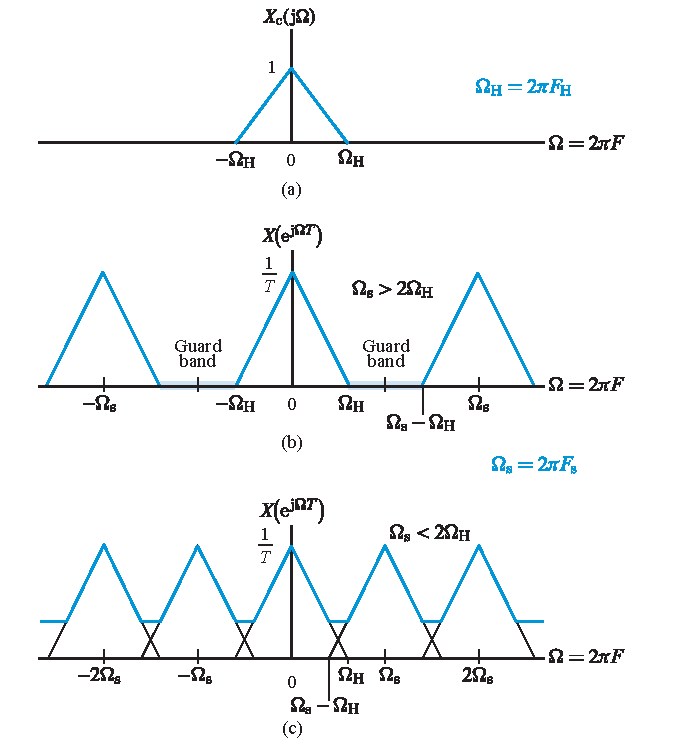
\includegraphics[scale=0.4]{Figures/Sampling/Impulse_Sampling_Effect}
\caption{Impulse Sampling Effect in the frequency spectrum \cite{DSP_DimitrisManolakis}}
\label{fig:Sampling:impulse_sampling_spectrum_1}
\end{figure}


\end{frame}


\subsection{Terminology and Definitions in Sampling}

\begin{frame}[t,allowframebreaks]{Terminology in Sampling Operation \cite{DSP_DimitrisManolakis}}

\begin{figure}[h]
\centering
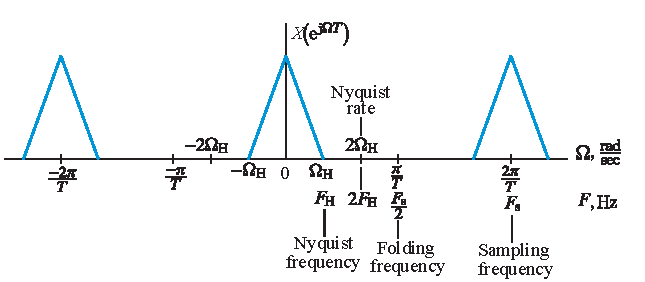
\includegraphics[scale=0.9]{Figures/Sampling/Impulse_Sampling_Terminology}
\caption{Replicated Amplitude Spectrum: Frequency axis in $F$[Hz] and $\omega_c$[rad/s] \cite{DSP_DimitrisManolakis}}
\label{fig:Sampling:Impulse_Sampling_Terminology}
\end{figure}

\newpage
\begin{itemize}

\item Highest Frequency $F_H$ in Hz presented in the continuous time signal $x_c(t) \rightarrow$ \textcolor{red}{Nyquist Frequency}

\item \textcolor{red}{Minimum sampling frequency} required to avoid overlapping bands $\rightarrow$ \textcolor{red}{Nyquist Rate}

\item Actual highest frequency that the sampled signal $x[n]$ contains is $\displaystyle\frac{F_s}{2} \, \rightarrow$ \textcolor{red}{folding frequency} 
 
\end{itemize}

\end{frame}


\subsection{Sampling Example}
\begin{frame}[t]{Sampling Effect Example}

To regenerate the pictures later.

\end{frame}

\subsubsection{Aliasing of Cos Signal}

\begin{frame}[t,allowframebreaks]{Aliasing of Cos Signal}

\begin{figure}[h]
\centering
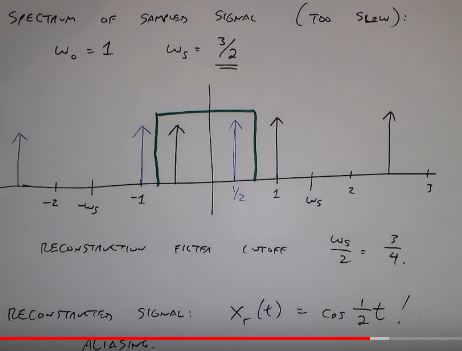
\includegraphics[scale=0.6]{Figures/Sampling/cos_signal_aliasing}
\label{fig:Sampling:cos_aliasing}
\end{figure}

\newpage
\begin{itemize}

\item The low pass filter is from $\displaystyle\frac{-\omega_s}{2} \, \rightarrow \, + \, \displaystyle\frac{+\omega_s}{2}$

\item Because we undersampled (not respect the Nyquist criterion), the DAC construct an aliased cos signal

\end{itemize}


\end{frame}

\subsection{Reconstruction}
\begin{frame}[t,allowframebreaks]{Reconstruction of Baseband Continuous time signal}

\begin{itemize}
\item Goal now: \textcolor{red}{restore} our \textcolor{red}{original signal} from our samples
	
	\begin{itemize}
	\item In other words, undo the effect of sampling
	\end{itemize}

\begin{figure}[h]
\centering
\includegraphics[scale=0.550]{Figures/Sampling/reconstruction_problem}
\caption{Reconstruction from samples: which version to choose \cite{DSP_DimitrisManolakis}}
\end{figure}

\item Working Conditions:

	\begin{itemize}
	\item Assuming that the signal is \textcolor{red}{bandlimited}

	\item Practicle sampling and reconstruction to be done later (like ZOH)
		
	\item Neglecting the effect of quantization for now
	
	
	\end{itemize}

\item This can be done from frequency domain perspective:

	\begin{itemize}
	\item Filtering the original spectrum and reject the images (replications)
	
	\end{itemize}

\item After the proof (to be put later in details) we get:
	
	\begin{equation}
	\hat{x}_{\text{sinc}}(t) \, = \, \displaystyle\sum\limits_{n \, = \, -\infty}^{+ \infty} x_{\text{sampled}} \left(\, n \, T_s \, \right) \text{sinc}\left[\, \displaystyle\frac{\omega_s \, \left(\, t \, - \,  n \, T_s \,\right)}{2}    \,\right]
	\label{Eq:Sampling:Ideal_Reconstruction}
	\end{equation}
	
	\begin{itemize}
	\item $\hat{x}_{\text{sinc}}(t)$ is the \textcolor{red}{sum of shifted sinc}, each \textcolor{red} {weighted} by a different amplitude $x(n \, T_s)$
	\end{itemize}

\end{itemize}

\end{frame}

\begin{frame}[t]{Visual Interpretation of Ideal Reconstruction 1}

\begin{figure}[h]
\centering
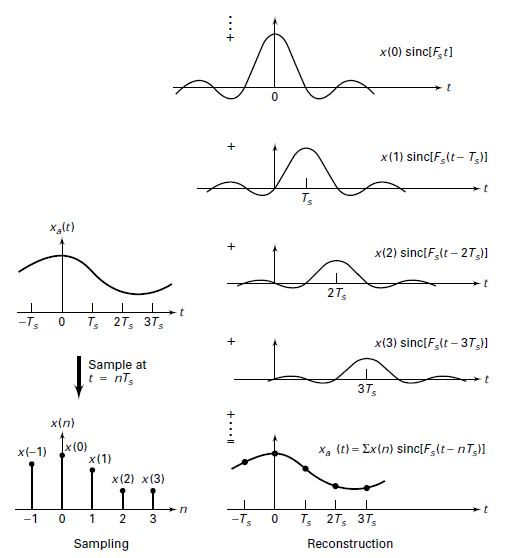
\includegraphics[scale = 0.4]{Figures/Sampling/ideal_bandlimited_interpolation_1}
\caption{Reconstruction of band-limited signal from its samples \cite{DSP_Matlab_Proakis}}
\end{figure}

\end{frame}

\begin{frame}[t]{Visual Interpretation of Ideal Reconstruction 2}

\begin{figure}[h]
\centering
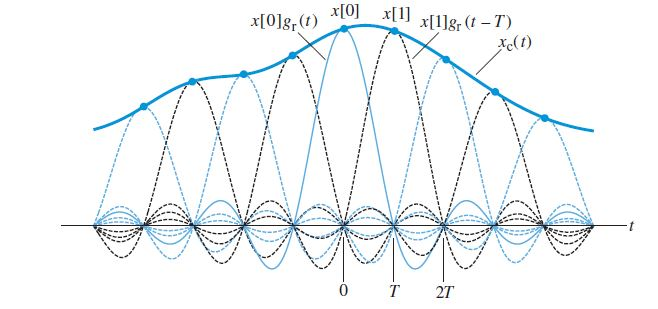
\includegraphics[scale=0.550]{Figures/Sampling/ideal_bandlimited_interpolation}
\caption{Ideal bandlimited interpolation in the time domain \cite{DSP_DimitrisManolakis}}
\end{figure}

\end{frame}


\subsection{Excercice On Ideal Sinc Interpolation}

\begin{frame}[t,fragile]{Implementation of Sinc Interpolation}

\begin{itemize}

\item If we want to implement equation (\autoref{Eq:Sampling:Ideal_Reconstruction}), we need to take care of 2 points:

	\begin{itemize}
	\item The Summation limit: we can't add from $-\infty \rightarrow \, +\infty$, so we need to truncate and choose some grid of discrete samples from $n \, = n_{\text{start} } \rightarrow n_{\text{finish} }$
	
	\item The $t$ is also need to be discretized on some grid: $t \, \approx \,$ \verb|t-start:step:t-end|
	\end{itemize}

\end{itemize}

\end{frame}


\subsection{Practical Reconstruction}
\begin{frame}[t,allowframebreaks]{Practical Reconstruction}

\begin{itemize}

\item Recap: Ideal reconstruction is done based on infinite sum of interpolated sinc 

\begin{equation}
	\hat{x}(t) \, = \, \displaystyle\sum\limits_{n \, = \, -\infty}^{+ \infty} x\left(\, n \, T_s \, \right) \text{sinc}\left[\, \displaystyle\frac{\omega_s \, \left(\, t \, - \,  n \, T_s \,\right)}{2}    \,\right]
	\label{Eq:Sampling:ideal_sinc_interpolation}
	\end{equation}
	
	
\item A more practical approach is based on ZOH \cite{signal_processing_Lathi}

\begin{figure}[h]
\centering
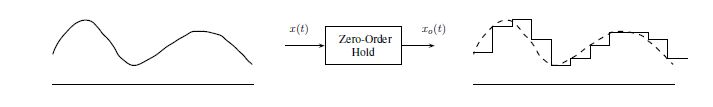
\includegraphics[scale=0.450]{Figures/Sampling/sampling_zoh}
\caption{Sampling using ZOH}
\label{fig:Sampling:sampling_zoh}
\end{figure}

\newpage
\item Implementation:

\begin{itemize}
	\item Let's denote the rectangular pulse we are using by $h(t)$ denoted by:

\begin{equation}
h(t)\, = \, \begin{cases}
1 \quad 0 \, \leq \, t \, \leq \, T_s \\
0 \quad \text{otherwise}
\end{cases}
\end{equation}

\item The $x_{\text{zoh}}$ can be written as:

\begin{equation}
x_{\text{zoh}} \, = \, \displaystyle\sum\limits_{n \, = \, -\infty}^{\infty} x(n) h\left(	t \, - \, n\,T_s \right)
\label{Eq:Sampling:Zoh_eq_1}
\end{equation}

\item Taking advantage from \textcolor{red}{convolution shifting property}: 
Recall that we can obtained a \textcolor{red}{shifted version of a signal} by \textcolor{red}{convolving this signal with a dirac function} so equation (\ref{Eq:Sampling:Zoh_eq_1}) can be further formulated

\begin{equation}
\begin{array}{rcl}
x_{\text{zoh}} \, &=& \, \displaystyle\sum\limits_{n \, = \, -\infty}^{\infty} x(n) \, h\left(	t \, - \, n\,T_s \right) \\ \\		
&=& \, \displaystyle\sum\limits_{n \, = \, -\infty}^{\infty} x(n) \, \times \, \left[ \, \delta \left(	t \, - \, n\,T_s \right) \, * \, h(t) \, \right] \\ 
\end{array}
\label{Eq:Sampling:Zoh_eq_2}
\end{equation}

\item Manipulating the parenthesis of equation (\ref{Eq:Sampling:Zoh_eq_2}):

\begin{equation}
\begin{array}{rcl}
x_{\text{zoh}} \, &=& \, \displaystyle\sum\limits_{n \, = \, -\infty}^{\infty} x(n) \, h\left(	t \, - \, n\,T_s \right) \\ \\		
&=& \, \displaystyle\sum\limits_{n \, = \, -\infty}^{\infty} x(n) \, \times \, \left[ \, \delta \left(	t \, - \, n\,T_s \right) \, * \, h(t) \, \right] \\ \\
&=& \, \displaystyle\sum\limits_{n \, = \, -\infty}^{\infty} \left[\, x(n) \, \times  \, \delta \left(	t \, - \, n\,T_s \right) \, \right] \, * \, h(t)   \\ \\
&=& \,  x_{\delta}(t) \, * h(t)
\end{array}
\label{Eq:Sampling:Zoh_eq_3}
\end{equation}

\begin{figure}[h]
\centering
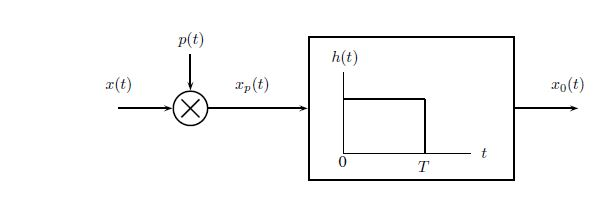
\includegraphics[scale=0.450]{Figures/Sampling/zoh_math}
\caption{Mathematical modeling of the ZOH}
\label{fig:Sampling:zoh_math}
\end{figure}

\item Implication on Spectrum:

\begin{figure}[h]
\centering
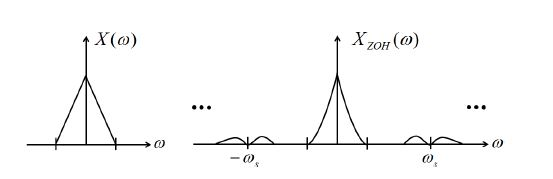
\includegraphics[width = 0.7\textwidth]{Figures/Sampling/zoh_output_spectrum}
\caption{Output of ZOH in the frequency domain}
\label{fig:Sampling:zoh_output_spectrum}
\end{figure}


\begin{itemize}

\item In impulse sampling (see figure \autoref{fig:Sampling:impulse_sampling_spectrum_1}), the spectrum was the same (with the scale factor $\displaystyle\frac{1}{T_s}$), along with the replicate at multiple of $\omega_s$.


\item In ZOH, these \textcolor{red}{replicate are attenuated} due to the low pass nature of the ZOH, which is a good thing since we don't want these images.

\item However, the \textcolor{red}{original spectrum is getting distorted}, and this distortion is controlled by the time sampling we choose to get our values. 

\end{itemize}

\end{itemize}

\item Antimaging-filter: to smooth the effect of the ZOH

\begin{figure}[h]
\centering
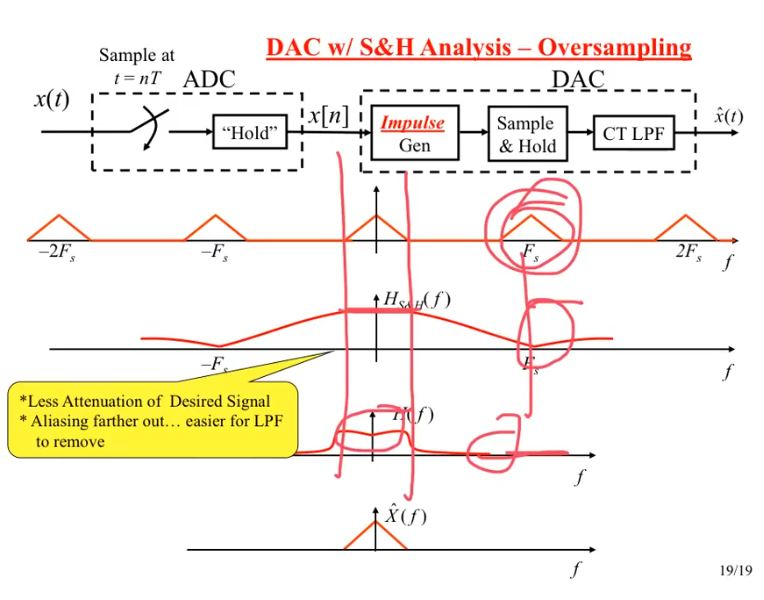
\includegraphics[width = 0.7\textwidth]{Figures/Sampling/oversampling_benefits}
\caption{Over sampling Benefits}
\label{fig:Sampling:oversampling_benefits}
\end{figure}

\begin{itemize}

\item Make the frequency response of the ZOH system more flat in the pass band

\item Easier transition band design for the smoothing filter

\end{itemize}

\item Didn't Grasp yet: people do \textcolor{red} {resampling}(upsampling and Multirate sampling techniques)at $x[n]$ to make the design more easier (didn't do it yet)

\end{itemize}

\end{frame}


%***********************************
%***********************************
%***********************************




\section{Bandpass Sampling}
\label{Chap:Bandpass_Sampling}
\begin{frame}[t]{Chapter \autoref{Chap:Bandpass_Sampling}}
\tableofcontents[sections= \value{section}]
\end{frame}



\subsection{Introduction}

\begin{frame}[t,allowframebreaks]{Introduction and Motivation}

\begin{itemize}

\item Based on Paper of \cite{Sub_Nyquist_sampling}\footnotemark and textbooks \cite{DSP_Proakis}, \cite{DSP_practical_approach}, and \cite{book_understanding_dsp}
\footnotetext[1]{Sub-Nyquist Sampling,Bridging theory and Practice, By Moshe Mishali and Yonina C. Eldar,IEEE SIGNAL PROCESSING MAGAZINE,NOVEMBER 2011}

\item By bandpass signals $\leftrightarrow$ amplitude spectrum isn't centered at 0 Hz \cite{book_understanding_dsp}

	\begin{itemize}
	\item Instead, the spectrum is centered at some frequency $f_{\text{center}} \, \neq \, 0$ Hz \cite{book_understanding_dsp}
	
	\item Such signals are encountered in RF application (communication and radar)
	\end{itemize}

\item An example of such signals is shown in figure \autoref{fig:Bandpass_Sampling:multiband_signals}

\newpage
\begin{figure}[h]
\centering
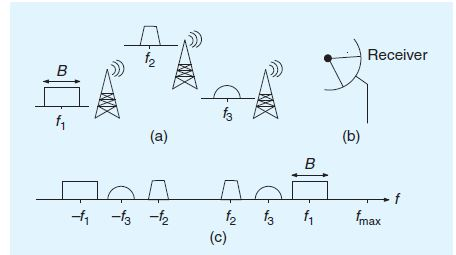
\includegraphics[scale = 0.4]{Figures/Bandpass_Sampling/multiband_signals}
\caption{Parts (a)–(c) show three RF transmissions with different carriers $f_i$. In (c), the receiver sees a multiband signal \cite{Sub_Nyquist_sampling}}
\label{fig:Bandpass_Sampling:multiband_signals}
\end{figure}

	\begin{itemize}
	\item The amplitude spectrum is centered at a center frequency $f_{\text{center}}$
	\end{itemize}


\end{itemize}

\end{frame}

\begin{frame}[t]{Parameters of a Bandpass Signal}

\begin{figure}[h]
\centering
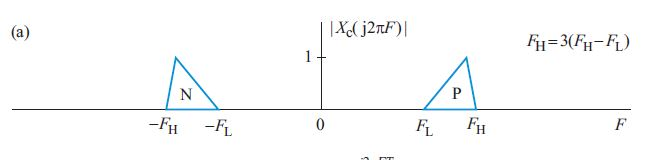
\includegraphics[scale = 0.4]{Figures/Bandpass_Sampling/bandpass_signal_example_2}
\caption{Amplitude Spectrum of a Bandpass Signal \cite{DSP_DimitrisManolakis}}
\label{fig:Bandpass_Sampling:bandpass_signal_example_2}
\end{figure}

\begin{itemize}

\item center frequency $f_{\text{center}}$
	
\item The bandwidth $B \, = \, f_{\text{high}} \, - \, f_{\text{low}} \, = \, f_{\text{upper}} \, - \, f_{\text{lower}} $ 
	 
\item Also any bandpass spectrum has a \textcolor{red}{positive and negative spectrum portion} since bandpass signals are reals signals
	 
\end{itemize}

\end{frame}


\begin{frame}[t]{Sampling a Bandpass Signals: Less than Nyquist rate}

\begin{itemize}

\item When we need to sample a bandpass signals, we could also apply the Nyquist theorem by setting $f_s \, = \, 2 \, \times \, f_{\text{upper}}$

\item However, $f_{\text{upper}}$ is usually big to any practical A/D converter

\item Instead, we can do sampling for such kind of signals in clever way by avoiding using such high frequencies


\item Advantages \cite{book_understanding_dsp}

	\begin{enumerate}
	\item Reduce \textcolor{red}{speed requirement of A/D converters} below that necessary in conventional low-pass sampling
	
	\item Reduce \textcolor{red}{amount of digital memory }necessary to capture a given time interval of a continuous signal
	\end{enumerate}


\item 2 methods to deal with sampling of such kind of signals:


	\begin{enumerate}
	\item Band-positioning
	
	\item Quadrature Sampling based on equivalent based band representation
	
	\end{enumerate}


\end{itemize}

\end{frame}


\subsection{Band positioning}
\begin{frame}[t]{Band positioning}

\begin{itemize}

\item What is band position ?

	\begin{itemize}
	\item It refers to the fractional number of bandwidths from the origin at which the lower band edge resides \cite{paper_bandpass_sampling_theory}.
	\end{itemize}

\item Unlike low-pass sampling, we are \textcolor{red}{interested in the signal bandwidth} rather by its highest frequency components

\item Instead of applying $F_s \geq \, 2 \, f_{\text{upper}}$, we will see that we can take $ 2 \, B \leq \, F_s \, \leq \, 4 \, B$

	\begin{itemize}
	\item Notice that we have gain allot by reducing $F_s$ from $ 2 \, f_{\text{upper}} \, \rightarrow \, [\,2 \, B \, ; \, 4 \, B \, ]$ because usually $f_{\text{upper}} >\, >\, B$
	
	\item Interesting thing that the range $2 \, B \leq \, F_s \, \leq \, 4 \, B$ implies that Nyquiste rate is always respected similar to the baseband case
	\end{itemize}

\end{itemize}

\end{frame}

\begin{frame}[t]{Integer Band positioning}

\begin{itemize}

\item We begin with a \textcolor{red}{special case} of \textcolor{red}{band positioning} technique known as \textcolor{red}{integer band positioning}

	\begin{itemize}
	\item $f_{\text{upper}}$ is an \textcolor{red}{integer multiple} of the \textcolor{red}{signal bandwidth} $B \, \leftrightarrow \, f_{\text{upper}} \, = \, K \, (f_{\text{upper}} \, - \, f_{\text{lower}}) \, = \, K \, B$ where $K \in \mathbb{N}$
	\end{itemize}


\item In this case, we can take $F_s \, = \, 2 \, B$ to sample this bandpass signal, and reconstruct without any distortion or aliasing

\item Ideal Interpolator (also known as \textcolor{red} {modulated interpolator}) formula in this case:

\begin{equation}
g_{\text{int}}(t) \, = \, \text{sinc}(B \, t) \, \text{cos}(2 \, \pi \, f_{\text{center}} \, t)
\end{equation}

\end{itemize}

\end{frame}


\begin{frame}[t]{Arbitrary band positioning}

\begin{itemize}
\item Now we move to a \textcolor{red}{more general case}, where  $f_{\text{upper}}$ isn't a multiple of the signal bandwidth $B$, a more general analysis is to be required


\item In this case, $F_s$ need to verify some  \textcolor{red}{constraints} translated by following \textcolor{red}{inequalities}:

\begin{equation}
\displaystyle\frac{2 \, f_{\text{upper}}}{k} \, \leq \, F_s \, \leq \, \displaystyle\frac{2 \, f_{\text{lower}}}{k \, - \, 1}
\end{equation}

\item In terms of $f_{\text{center}}$ and signal bandwidth $B$ we can write the above constraints as \cite{book_understanding_dsp}:

\begin{equation}
\displaystyle\frac{2 \, f_{\text{center}} \, + \, B}{k} \, \leq \, F_s \, \leq \, \displaystyle\frac{2 \, f_{\text{center}} \, - \, B}{k \, - \, 1}
\end{equation}

such that $f_{\text{center}} \, = \, \displaystyle\frac{f_{\text{lower}} \, + \, f_{\text{upper}}}{2}$


\end{itemize}

\end{frame}


\begin{frame}[t,allowframebreaks]{Graphical Interpretation}


\begin{itemize}

\item Graphical Interpretation:

\begin{figure}[h]
\centering
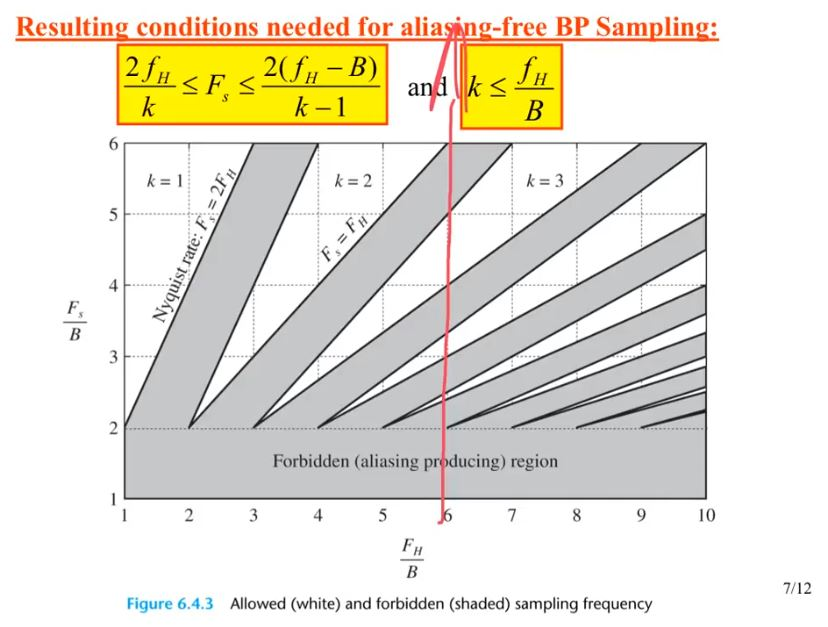
\includegraphics[scale = 0.3]{Figures/Sampling/bandpass_sampling_general_case_plots}
\caption{Bandpass sampling plot: $F_s$ function of $f_{\text{high}}$}
\label{fig:Sampling:bandpass_sampling_general_case_plots}
\end{figure}

	\item The plots are normalized over the bandwidth $B$, which makes plotting the equation more easy
	
	\item $k \, = \, 1$: we are operating on the standard Nyquiste rate
	
	
	\item if we have $\displaystyle\frac{f_{\text{high}}}{\text{ bandwidth}} \, = \, 6$, we can operate at multiple $k$: 1,2, 3 and 4 and even 5 (the higher $k$ the lower is $F_s$)
	
	\newpage
	\item However, we have to pay attention at $k \, = \, 5$
	
	\begin{figure}[h]
\centering
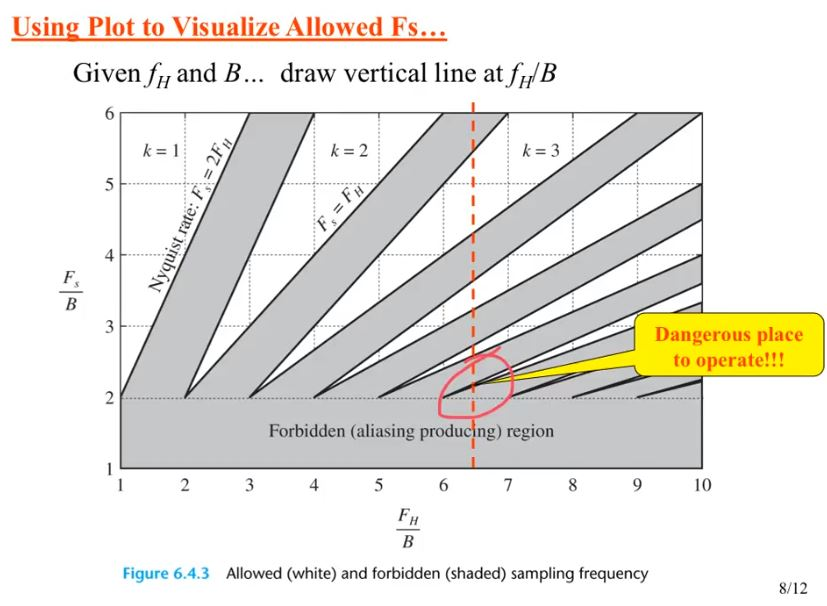
\includegraphics[scale = 0.3]{Figures/Sampling/bandpass_sampling_general_case_plots_2}
\caption{Bandpass sampling plot: dangerous area we need to pay attention from}
\label{fig:Sampling:bandpass_sampling_general_case_plots_2}
\end{figure}

	\item From this dangerous place, comes the idea of guard band shown in \autoref{fig:Sampling:bandpass_sampling_guard_bands}
	
	
	\begin{figure}[h]
\centering
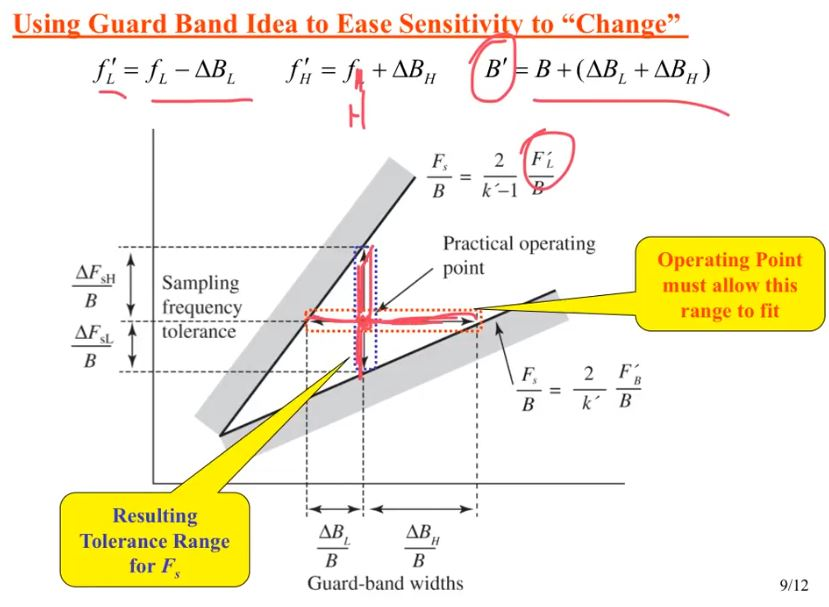
\includegraphics[scale = 0.3]{Figures/Sampling/bandpass_sampling_guard_bands}
\caption{Bandpass sampling plot:putting some guard bands}
\label{fig:Sampling:bandpass_sampling_guard_bands}
\end{figure}



\end{itemize}



\end{frame}


\subsection{Quadrature Sampling}
\begin{frame}[t,allowframebreaks]{Introduction In-phase and Quadrature Components of a Signal}

\begin{itemize}

\item \textcolor{red}{Before} we dive into what is called \textcolor{red}{qudarature sampling}, we begin by \textcolor{red}{explaining} what is so called \textcolor{red}{in-phase and quadrature representation (denoted by IQ) for a bandpass signal}

	\begin{itemize}
	\item These components will be used in quadrature sampling scheme
	\end{itemize}

\item From where the IQ components come from ?

\item Recall that when we have a bandpass signal, our target is to reduce the sampling rate $F_s$ and try to make as a function of the signal bandwidth $B$ rather than applying Nyquist rate directly (where it give us $F_s \, \geq \, 2 \, f_{\text{upper}}$)

	\begin{itemize}
	\item This what we have done in band positioning method
	\end{itemize}

\newpage
\item Another way to approach this problem, is to \textcolor{red}{shift the frequency spectrum} (say the postive part) and \textcolor{red}{centered about 0 Hz}, and make it a baseband signal
	
	\begin{itemize}
	\item In other words, we want to obtain an \textcolor{red}{equivalent low-pass signal} of the bandpass signal
	
	\item We do this because working with baseband representation is easier for DSP processing task
	
	\item This \textcolor{red}{equivalent low-pass signal} will contains the quadrature and in-phase component in which they will be used in bandpass signal representation
	\end{itemize}

\end{itemize}

\end{frame}


\begin{frame}[t]{Steps to be taken}

\begin{enumerate}

\item Derive the equivalent baseband representation of a bandpass signal

	\begin{itemize}
	\item This will give birth to IQ components
	\end{itemize}

\item Make the link between the bandpass signals and the in-phase and quadrature component

\item Use this new representation to do sampling

\item Reconstruction formula

\end{enumerate}


\end{frame}


\begin{frame}[t]{Steps to derive Equivalent Lowpass Signal for a Bandpass Signal}


\begin{figure}[h]
\centering
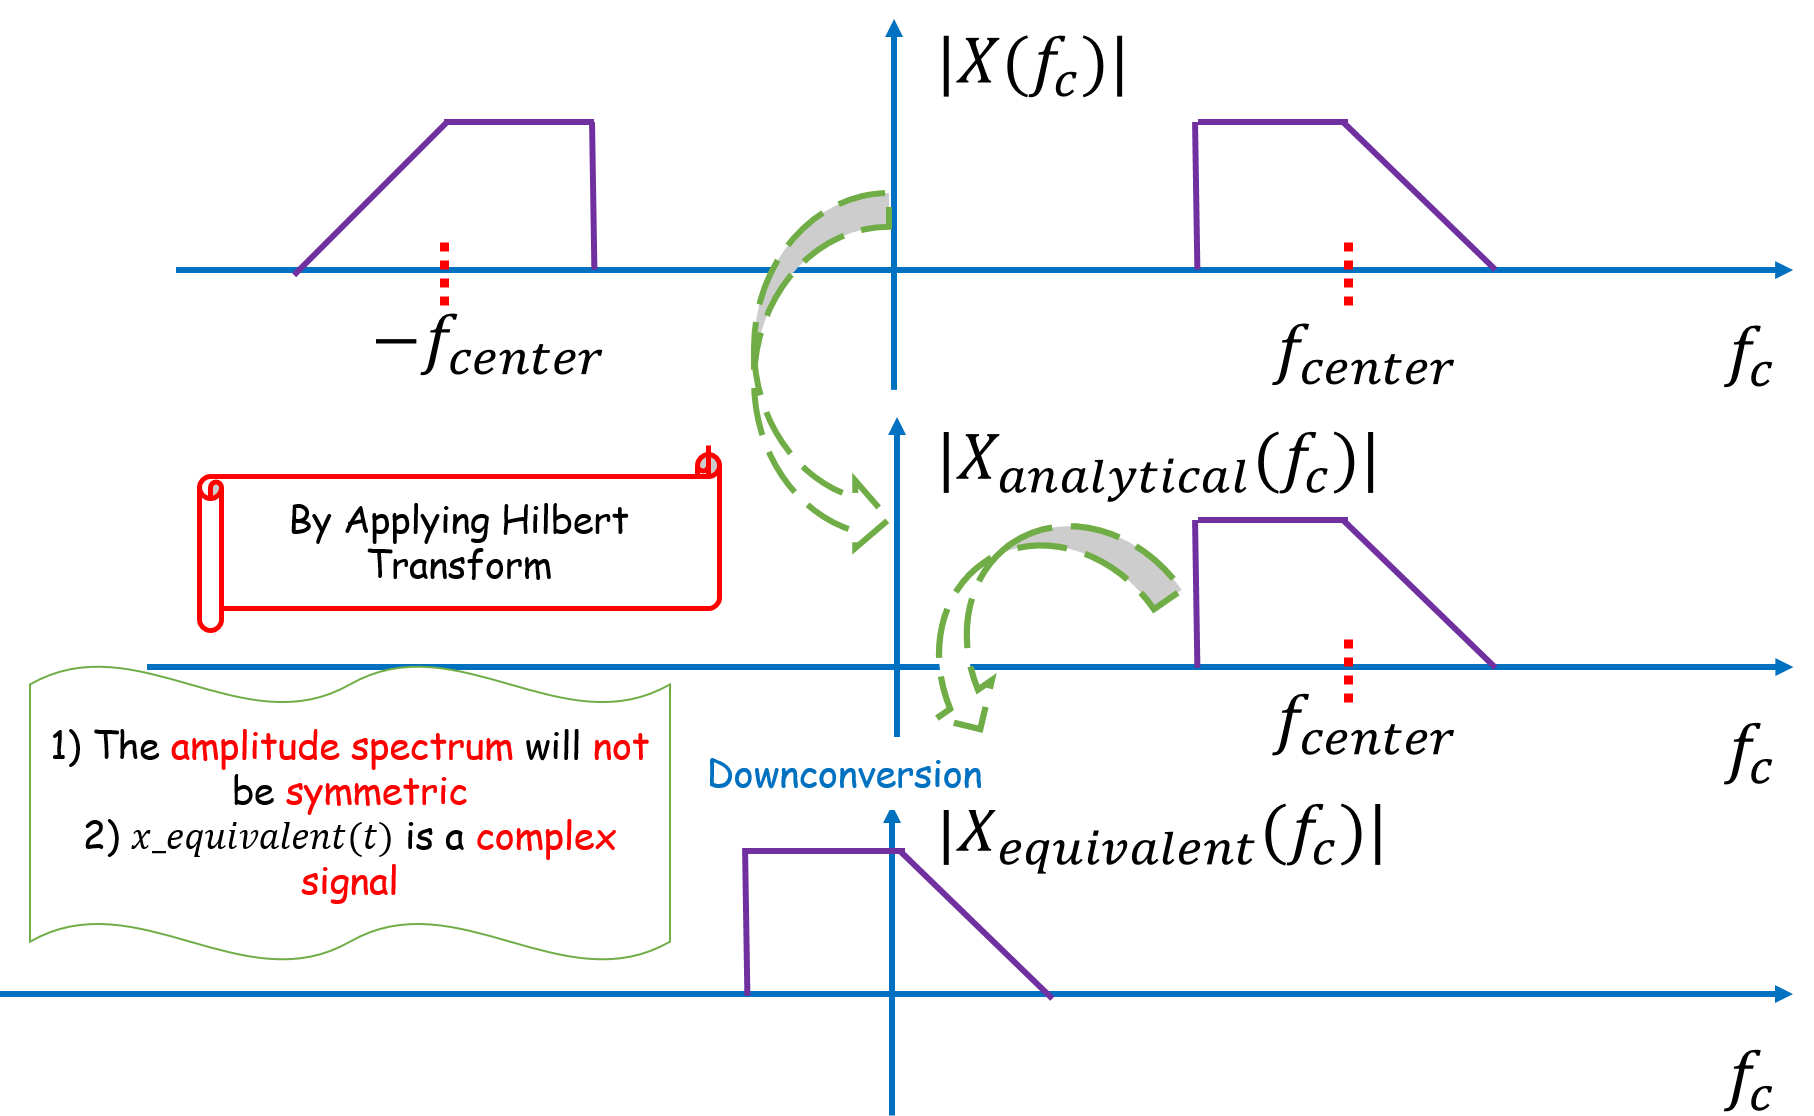
\includegraphics[scale = 0.35]{Figures/Bandpass_Sampling/equivalent_lowpass_signal_steps}
\label{fig:Bandpass_Sampling:equivalent_lowpass_signal_steps}
\end{figure}


\end{frame}


\begin{frame}[t,allowframebreaks]{Bandpass Signal Representation}

\begin{itemize}
	
\item \underline{Rule:}  Any \textcolor{red}{bandpass signal} can be written in terms of \textcolor{red}{in-phase and quadrature components} which are \textcolor{red}{complex baseband signals}
	
	
\item Sampling Each Component at a rate of $F_s$

\item Bandpass Signal Representation \cite{DSP_Proakis} \cite{paper_bandpass_sampling_theory}:

	\begin{equation}
\begin{array}{rcl}
x_{\text{band-pass}}(t) \, &=&\, \text{Amp}(t) \, \times \, \text{cos}\left(\, 2 \pi \, f_{\text{center}} \, t \, + \, \text{phase}(t) \,\right)\\ \\
&=&\, x_{\text{in-phase}}(t) \, \text{cos}\left( \, 2 \pi \, f_{\text{center}} \, t \,\right) \\
 && \, - \, x_{\text{quadrature}}(t) \, \text{sin}\left( \, 2 \pi \, f_{\text{center}} \, t \,\right)
\end{array}
\label{Eq:Sampling:based_band_general_form_time_domain_recap}
\end{equation}


\item In-phase and Quadrature Components:

	
	\begin{equation}
\begin{array}{rcl}
x_{\text{in-phase}}(t) \, &=& \, \text{Amp}(t) \, \times \, \text{cos}\left[\, \text{phase}(t) \, \right] \\ \\
x_{\text{quadrature}}(t) \, &=& \, \text{Amp}(t) \, \times \, \text{sin}\left[\, \text{phase}(t) \, \right] \\ \\
\end{array}
\label{Eq:Sampling:inpahse_quadrature_signals}
\end{equation}
	
	
\end{itemize}

\end{frame}


\begin{frame}[t,allowframebreaks]{Implementation}


\begin{figure}[h]
\centering
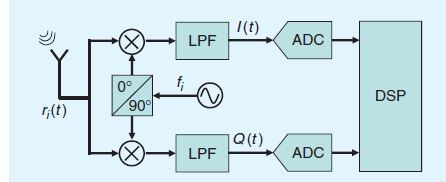
\includegraphics[width = 0.7\textwidth]{Figures/Sampling/I_Q_system}
\caption{A block diagram of a typical I-Q demodulator \cite{Sub_Nyquist_sampling}}
\label{fig:Sampling:I_Q_system}
\end{figure}

\begin{itemize}

\item The LPF is here due to high unwanted frequency components that we don't need them


\item Proofs: finish them on my initial report didn't have time to rewrite them from

\item Interpretation: Now we have 2 basedband signal (however remember that they are complex), and we can sample at a rate of  $F_s \, = \, B$ 

	\begin{itemize}
	\item But recall we have I and Q components
	
	\item So in total we have $F_s \, = \, 2 \, B$ 
	\end{itemize}

\item Application \cite{Sub_Nyquist_sampling}: This option is used in relay stations or regenerative repeaters
that decode the information I 1t 2, Q1t 2, use digital error correction algorithms, and then transform the signal back to high frequencies for the next transmission section
	
\end{itemize}
	
\end{frame}


\begin{frame}[t]{Band Positioning and IQ Comparison}

Note: to be put in a form of a table later

\begin{enumerate}

\item Band positioning:
	
	\begin{itemize}
	\item Can be applied directly to the signal $x(t)$ with no analog preprocessing hardware as in IQ
	
	\item But not suited for multiband signals
	\end{itemize}



\item IQ Demodulation

	\begin{itemize}
	\item Suitable for RF transmission which offers decoupling property of the dependency of the bandwidth of A/D on the maximal frequency of the input (like an RF transmitted signal) 
	
	
	\item Only in-band noise is inputted 
	\end{itemize}


\end{enumerate}


\end{frame}


\begin{frame}[t,allowframebreaks]{Integer band positioning}

\begin{itemize}



\item Thanks to the course of Dr.Mark Fowler, Binghmton University, State University of New York

	\begin{itemize}
	\item More pedagogical way to explain these concepts
	\end{itemize}



\begin{figure}[h]
\centering
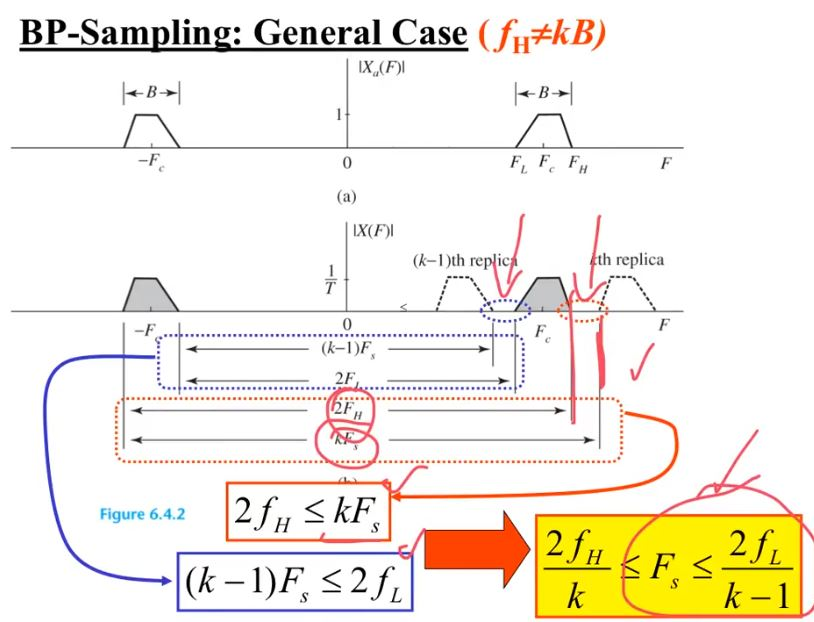
\includegraphics[width = 0.6\textwidth]{Figures/Sampling/bandpass_sampling_general_case_non_integer}
\caption{Bandpass sampling non integer case}
\label{fig:Sampling:bandpass_sampling_general_case_non_integer}
\end{figure}

\newpage
\item Equations:

\begin{equation}
\begin{array}{rcl}
\displaystyle\frac{2 \, f_{\text{high}}}{k} \, &\leq& \, F_s \,\, \, \, \leq \, \displaystyle\frac{2 \,\left( \,  f_{\text{high}} \, - \, \text{Bandwidth} \, \right)}{k \, - \, 1} \\ \\
k \, &\leq& \, \displaystyle\frac{2 \, f_{\text{high}}}{\text{Bandwidth}} 
\end{array}
\label{Eq:Sampling:bandpass_sampling_bounds}
\end{equation}

\item Graphical Interpretation:

Plotting equations (\ref{Eq:Sampling:bandpass_sampling_bounds}) give us plot shown in \autoref{fig:Sampling:bandpass_sampling_general_case_plots}.


\begin{figure}[h]
\centering
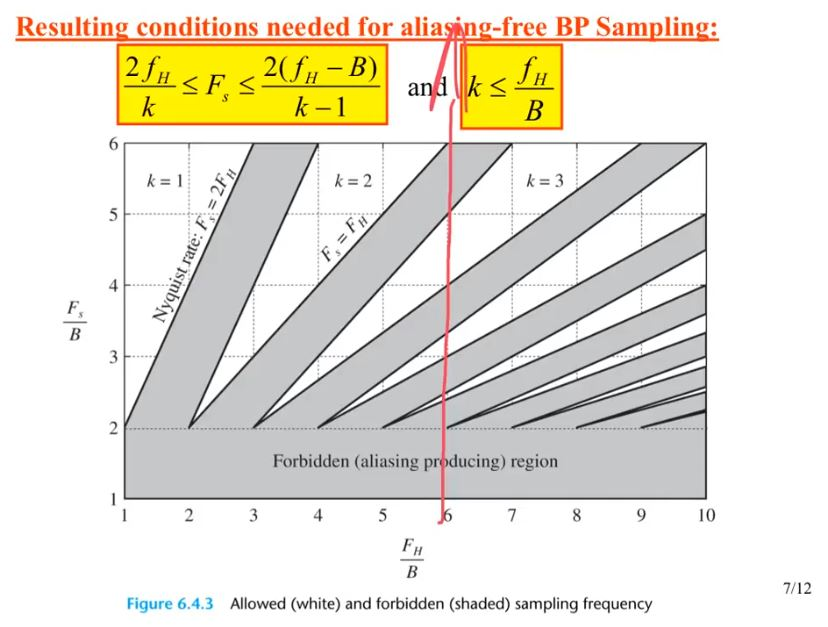
\includegraphics[width = 0.7\textwidth]{Figures/Sampling/bandpass_sampling_general_case_plots}
\caption{Bandpass sampling plot: $F_s$ function of $f_{\text{high}}$}
\label{fig:Sampling:bandpass_sampling_general_case_plots}
\end{figure}

	\begin{itemize}
	\item The plots are normalized over the bandwidth $B$, which makes plotting the equation more easy
	
	\item $k \, = \, 1$: we are operating on the standard Nyquiste rate
	
	
	\item if we have $\displaystyle\frac{f_{\text{high}}}{\text{ bandwidth}} \, = \, 6$, we can operate at multiple $k$: 1,2, 3 and 4 and even 5 (the higher $k$ the lower is $F_s$)
	
	\newpage
	\item However, we have to pay attention at $k \, = \, 5$
	
	\begin{figure}[h]
\centering
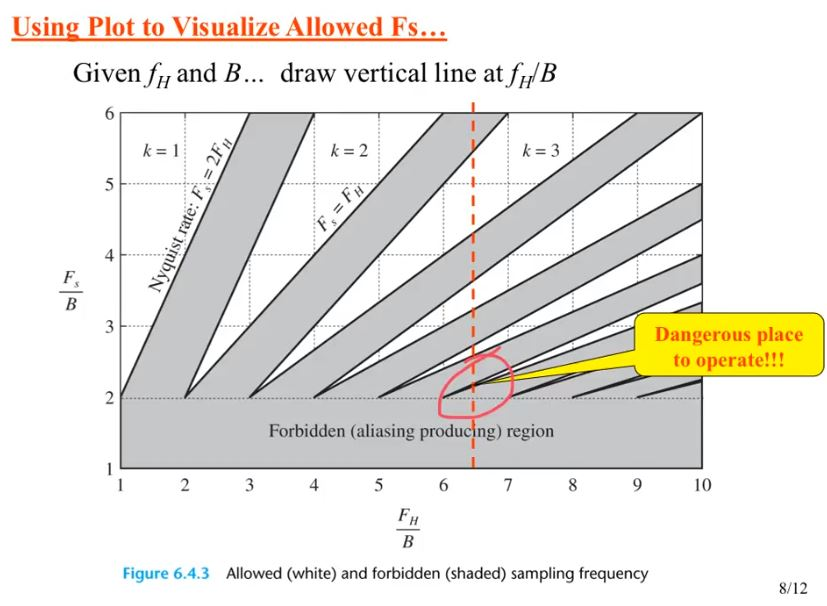
\includegraphics[width = 0.7\textwidth]{Figures/Sampling/bandpass_sampling_general_case_plots_2}
\caption{Bandpass sampling plot: dangerous area we need to pay attention from}
\label{fig:Sampling:bandpass_sampling_general_case_plots_2}
\end{figure}

	\item From this dangerous place, comes the idea of guard band shown in \autoref{fig:Sampling:bandpass_sampling_guard_bands}
	
	
	\begin{figure}[h]
\centering
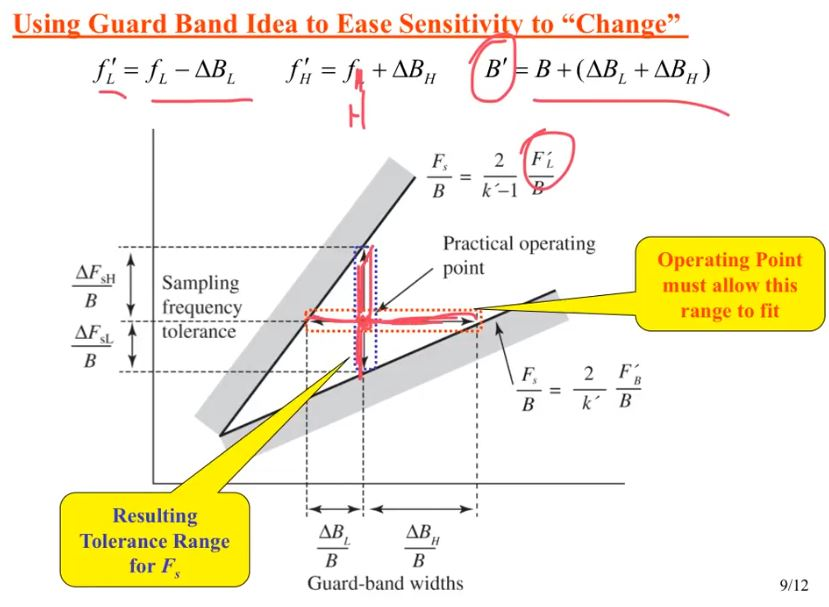
\includegraphics[width = 0.7\textwidth]{Figures/Sampling/bandpass_sampling_guard_bands}
\caption{Bandpass sampling plot:putting some guard bands}
\label{fig:Sampling:bandpass_sampling_guard_bands}
\end{figure}
	
	\end{itemize}



\end{itemize}


\end{frame}

\section{Frequency Relationship}
\label{Chap:Frequency Relationship}
\begin{frame}[t]{Chapter \autoref{Chap:Frequency Relationship}}
\tableofcontents[sections = \value{section}]
\end{frame}

\begin{frame}[c]
% c for center

\begin{center}
\Huge \textcolor{green}{Frequency Relationship}
\end{center}

\end{frame}

\subsection{Analog and Discrete Frequencies}
\begin{frame}[t,allowframebreaks]{Analog and Discrete Frequency Relationship}

\begin{itemize}

\item $ -\infty < \, \omega_c \left(\text{rad/sec}\right) \, < \, + \infty \, \leftrightarrow$ analog frequency

\item $ - \pi < \, \omega_d \left(\text{rad}\right) \, < \, + \pi \, \leftrightarrow$ discrete frequency

\end{itemize}

\begin{equation}
\begin{array}{rcl}
\omega_c \left(\text{rad/sec}\right) \, &=& \, \omega_d \, \times \, F_s \\ \\
&=& \, \displaystyle\frac{\omega_d}{T_s}  \\ \\

\omega_d \, &=& \, \omega_c \left(\text{rad/sec}\right) \, \times \, T_s \\ \\
&=& \, \displaystyle\frac{\omega_c}{F_s}
\end{array}
\label{Eq:Freq_relation:analog_discrete_freq}
\end{equation}



\end{frame}


\subsection{DTFT and Ideal Impulse CTFT Relation}
\begin{frame}[t]{DTFT and Ideal Impulse CTFT Relation}

\begin{itemize}

\item Small Recall:

	\begin{itemize}
	\item When we sample a signal in time domain, the original spectrum will get replicated: $X(f_c) \, \rightarrow \, \text{time domain sampling} \rightarrow X_{\delta}(f_c)$
	
		\begin{itemize}
		\item $X_{\delta}(f_c)$ is replicated at multiple of $F_s$ 
		\item Don't forget that we have a scaling amplitude factor $= \, \displaystyle\frac{\text{Amp}}{T_s}$
		\end{itemize}
	
	\item Now if we have a discrete signal $x[n]$, its DTFT $X(f_d)$ is replicated at multiple of $2 \pi$
	
		\begin{itemize}
		\item However, don't forget we have a relation between Sampled CTFT $X_{\delta}(f_c)$ and the DTFT $X(f_d)$ using equation (\autoref{Eq:Freq_relation:analog_discrete_freq})
			
	
	\end{itemize}

\end{itemize}

\end{itemize}

\end{frame}

%**************************************************
%**************************************************
%**************************************************
\section{Discrete Fourier Transform}
\label{Chap:DFT}
\begin{frame}[t,allowframebreaks]{Chapter \autoref{Chap:DFT}}
\tableofcontents[sections= \value{section}]
\end{frame}

\subsection{DFT Theory}
\begin{frame}[t]{DFT Theory}

To be done later.

\end{frame}

\subsection{Summary of DFT for CTFT and DTFT}
\begin{frame}[t]{DFT Different study cases and parameters}

\begin{figure}[h]
\centering
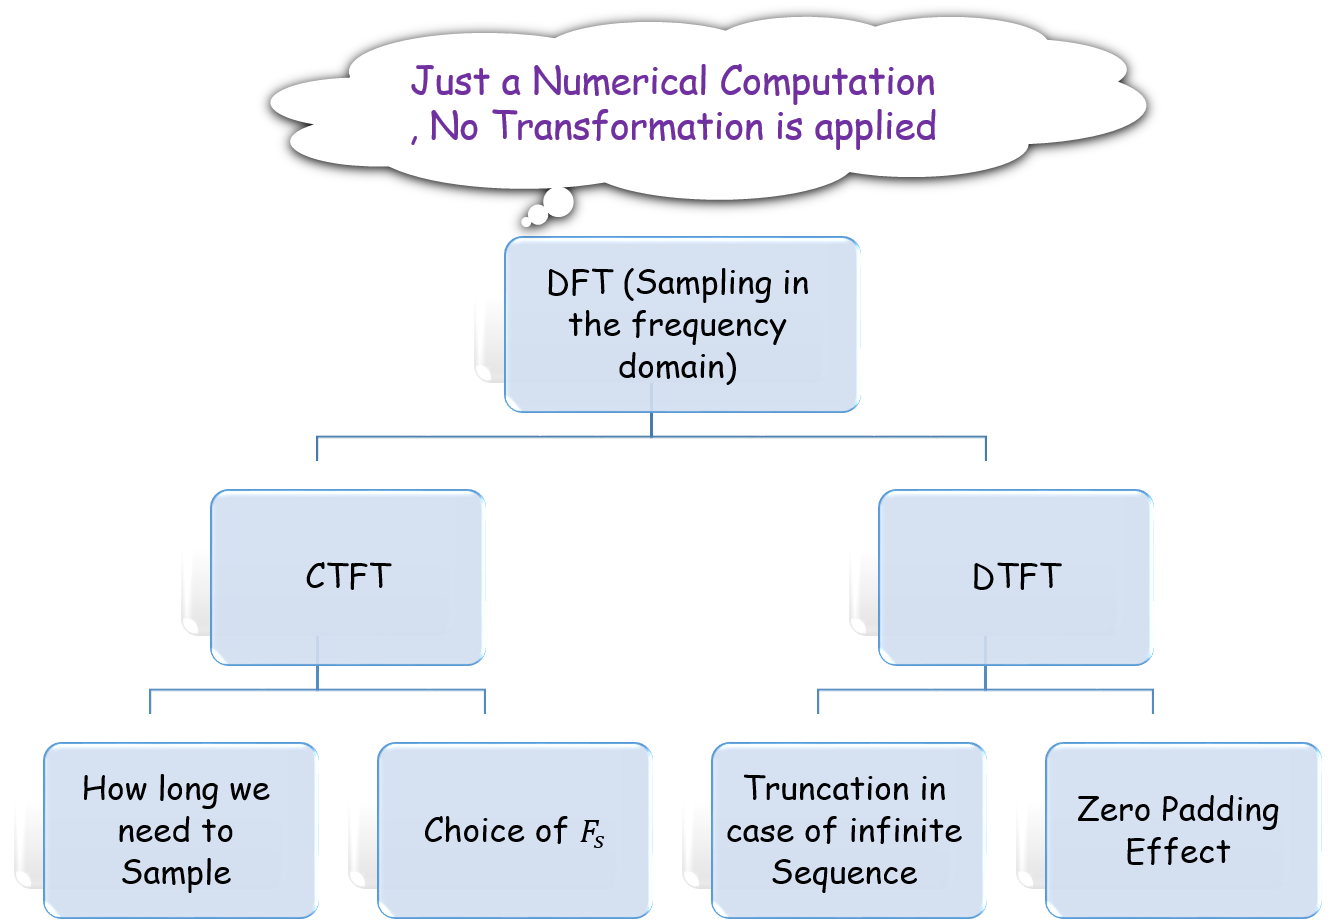
\includegraphics[width = 0.8\textwidth]{Figures/DFT/DFT_Idea}
\label{fig:DFT:DFT_Idea}
\end{figure}

\end{frame}


\begin{frame}[t,allowframebreaks]{DFT Formula for CTFT and DTFT}

\begin{columns}
\column{0.5\textwidth}

\begin{itemize}

\item \underline{CTFT Case:}

\item Let $f(t)$ be a continuous time signal of duration $\tau$.

\item Sample the signal $f(t)$ over a period $T_0 \, \leq \, \tau$, where $T_s$ is the sampling time. 

	\begin{itemize}
	\item The \tbi{number of sample} we get is $N_0 \, = \, \displaystyle\frac{T_0}{T_s} \, = \, T_0 \, \times \, F_s$
	\end{itemize}
\end{itemize}

\column{0.5\textwidth}

\begin{itemize}

\item \underline{DTFT Case:}

\item Let $f[k]$ a discrete signal with index $k$, of length $N_0$.

\item Sampling is already done since we are in discrete time domain.


\end{itemize}

\end{columns}

\end{frame}


\begin{frame}[t,allowframebreaks]{DFT Formula for CTFT and DTFT}

\begin{minipage}{\textwidth}


\begin{itemize}

\item Formula CTFT case:

\begin{equation}
\begin{array}{rcl}
\text{DFT}\{f[t]\} \, &=&\, F_r \\
						&=& \, F(r \, \omega_0) \\
					   &=&\, \displaystyle\sum_{k \, = \, 0}^{N_0 \, - \, 1} \, f_k \, \text{exp} \left(\, -j r \Omega_0 \, k   \,\right)
\end{array}
\end{equation}

where $\begin{cases}

\omega_0 \, = \, 2 \, \pi \, F_0 \, \text{rad/s} \, (\text{from spectral sampling theorem}) \\
\Omega_0 \, = \, \omega_0 \, T_s \, = \,   \displaystyle\frac{2 \, \pi}{N_0} \, = \, \text{sampling interval at wihich } \\
\text{we sample the spectrum of the CTFT} \\
f_k \, = \, T_s \, f(k \, T_s)
\end{cases}$ 


\end{itemize}


\end{minipage}


% 2nd column
\begin{minipage}{\textwidth}


\begin{itemize}



\item Formula DTFT case:

\begin{equation}
\begin{array}{rcl}
\text{DFT}\{f[k]\} \, &=&\, F_r \\
						&=& \, F(r \, \Omega_0) \\
					   &=&\, \displaystyle\sum_{k \, = \, 0}^{N_0 \, - \, 1} \, f[k] \, \text{exp} \left(\, -j r \Omega_0 \, k   \,\right)
\end{array}
\label{Eq:DFT:dft_for_dtft}
\end{equation}

where $\begin{cases}
r \, = \, 0,1,2, \rightarrow \, N_0 \, - \, 1 \\
\Omega_0 \, = \,  \displaystyle\frac{2 \, \pi}{N_0} \, = \, \text{freqeuncy step at which}\\
\text{we sample the DTFT spectrum}
\end{cases}$\\

\item  \underline{Inverse DFT case:}

\begin{equation}
\begin{array}{rcl}
f[k] \, &=&\, \displaystyle\frac{1}{N_0} \, \displaystyle\sum_{r \, = \, 0}^{N_0 \, - \, 1} \, F_r \, \text{exp} \left(\, -j r \Omega_0 \, k   \,\right)
\end{array}
\end{equation}

\end{itemize}

\end{minipage}


\end{frame}




\begin{frame}[t]{Analysis and Simulation on DFT Parameters for CTFT and DTFT}

\begin{itemize}

\item In the upcoming slides, we do several cases on DFT parameters in the continuous and discrete time domain

	\begin{enumerate}
	\item Example of computing CTFT with an infinite duration
	
	\item Example of computing DTFT with finite duration
	
	\end{enumerate}


\end{itemize}


\end{frame}

\subsection{DFT on CTFT for Infinite Time Duration Signal}



\subsubsection{Modeling}
\begin{frame}[t,allowframebreaks]{Time Truncation Choice}

\begin{itemize}


\item Signal to be taken:

\begin{equation}
x(t) \, = \, \text{exp}(-0.5 \, t) \, u(t) \leftrightarrow \, X(\omega_c) \, = \, \displaystyle\frac{1}{j \, \omega_c\, + \, 0.5}
\label{fig:Simulation_Sampling_Frequency_Analysis:infinite_cont_time}
\end{equation}

\item Signal of equation (\autoref{fig:Simulation_Sampling_Frequency_Analysis:infinite_cont_time})  is an \textcolor{red}{infinite continuous time and bandwidth signal}: no maximum frequency to be taken to apply Nyquist sampling theorem $\rightarrow$ need to \textcolor{red}{truncate in time so we can choose a sampling frequency}

	\begin{itemize}
	\item Criteria to truncation: what is the value of $\omega$ at which the frequency content is bellow 2 \% ? $\leftrightarrow$ capture 98 \% of the frequency content of the signal
	
	\item \underline{Computations:} $ \displaystyle\left\lvert X(\omega_c) \displaystyle\right\rvert \, = \, \displaystyle\frac{1}{\sqrt{ \omega^2_c\, + \, 0.5^2} } \, = \, 2 \, \times \, 0.01  \rightarrow \omega_c \, = \, 50 \text{ rad/s} \leftrightarrow \, B \, = \,  \displaystyle\frac{25}{\pi} \, \approx \, 8$ Hz so we get $T_s \, = \, \displaystyle\frac{\pi}{50}$ seconds
	\end{itemize}

\end{itemize}

\end{frame}

\begin{frame}[t,allowframebreaks]{Repeating Sampling}

\begin{itemize}

\item After we solve for $T_s \, = \, \displaystyle\frac{\pi}{50}$ s, there is another question to be asked: for \textcolor{red}{how long do we need to sample} ?

	\begin{itemize}
	\item This signal is going forever, we can't just keep sampling forever
	\end{itemize}

\item So we need to solve for \textcolor{red}{sampling duration} $T_0$

	\begin{itemize}
	\item \underline{Criteria to solve the problem:} We know that the signal is a decaying exponential, we can see for some value of $T_0$ where the  \textcolor{red}{amplitude value of the signal} $x(t)$  \textcolor{red}{are very low}, and by this we are  \textcolor{red}{not throwing some high value amplitude (information)}
	
	\item Computing: 
	
	\begin{itemize}
	\item We try for example for $T_0 \, = \, 16$s, we get $x(16) \, = \, e^{-0.5 \, (16)} = \, e^{-8} \, = \, 3.3 \, e^{-4}$, very small number
	
	\item If we choose $T_0 \, = \, 16$, the number of sample we get in this period using a sampling rate $T_s \, = \, \displaystyle\frac{\pi}{50}$ is: $N_0 \, = \, \displaystyle\frac{T_0}{T_s} \, = \, 254.65$
	
	
	\item However, the number of samples we need to grab need to be integer, so let's say we need to grab 256 samples
	
	\item We resolve again for $T_s$ using $N_0 \, = \, 256$ samples, and we get $T_s \, = \, \displaystyle\frac{1}{16}$ seconds 
\end{itemize}		
	
	\end{itemize}

\item The rest is done via programming part

\item As a \textcolor{red}{summary} we have:

\begin{itemize}

\item $\mathrm{1}^\mathrm{st}$ question we ask since the signal $x(t)$ isn't band limited in the frequency domain: \textcolor{red}{how do we choose the sampling period (sampling rate)} $T_s \, (F_s)$

	\begin{itemize}
	\item $T_s \, = \, \displaystyle\frac{1}{16}$ seconds
	\end{itemize}
https://www.overleaf.com/project/61346dff13f6cea26f81d723	
\item $\mathrm{2}^\mathrm{nd}$ question: for \textcolor{red}{how long we keep sampling $\leftrightarrow$ (signal truncation)} ?

	\begin{itemize}
	\item $T_0 \, = \, 16$ s, which give $N_0 \, = \, 256$ samples in the signal duration,
	such that $T_s \, = \, \displaystyle\frac{1}{16}$ s
	\end{itemize}

\end{itemize}


\end{itemize}


\end{frame}

\subsubsection{Results and Analysis}
\begin{frame}[t,allowframebreaks]{Results and Analysis}

\begin{figure}[h]
\centering
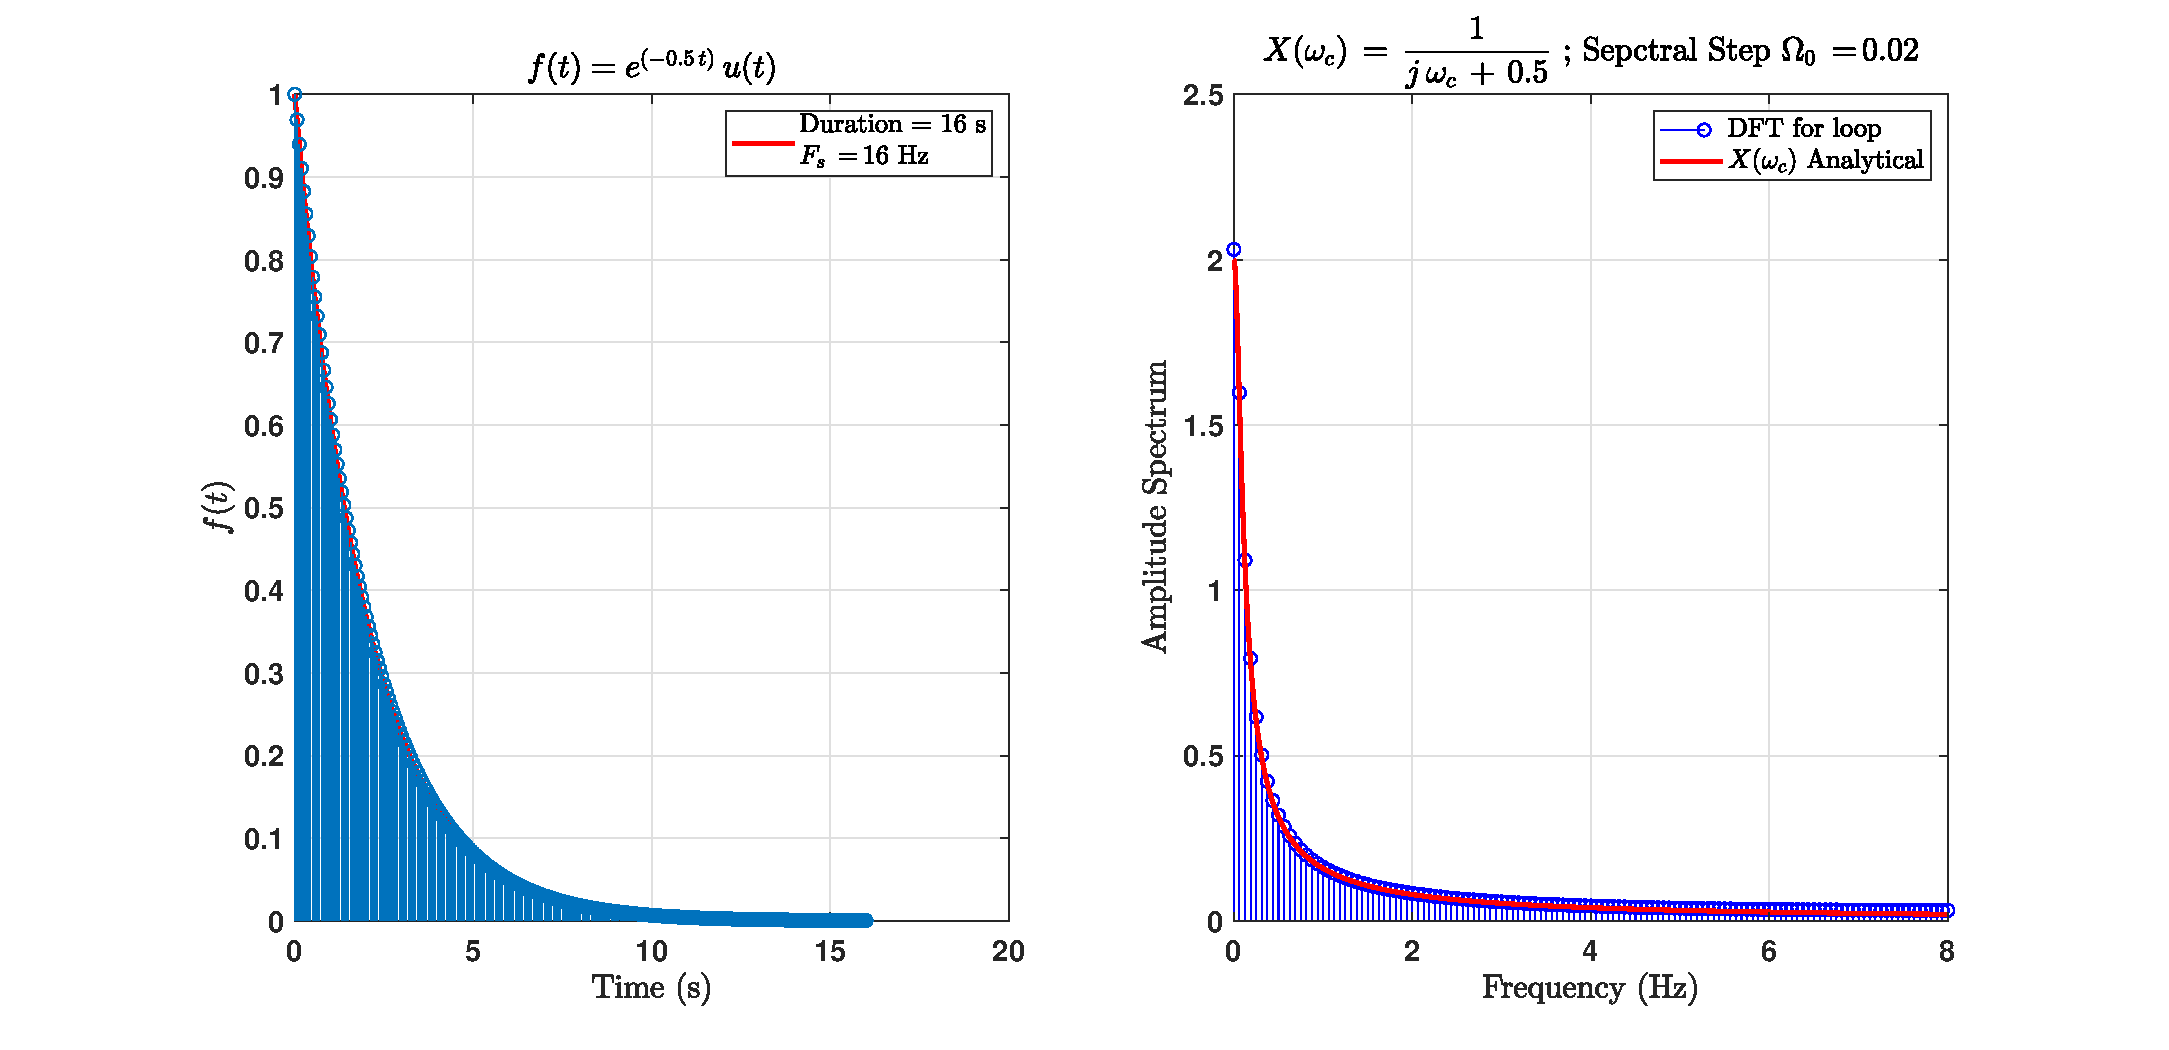
\includegraphics[scale = 0.30]{Figures/DFT/DFT_CTFT_duration_16}
\label{fig:Simulation_Sampling_Frequency_Analysis:DFT_CTFT_16}
\caption{Base line: Signal Duration is 16 s and $F_s \, = \,$ 16 Hz}
\end{figure}



\begin{figure}[h]
\centering
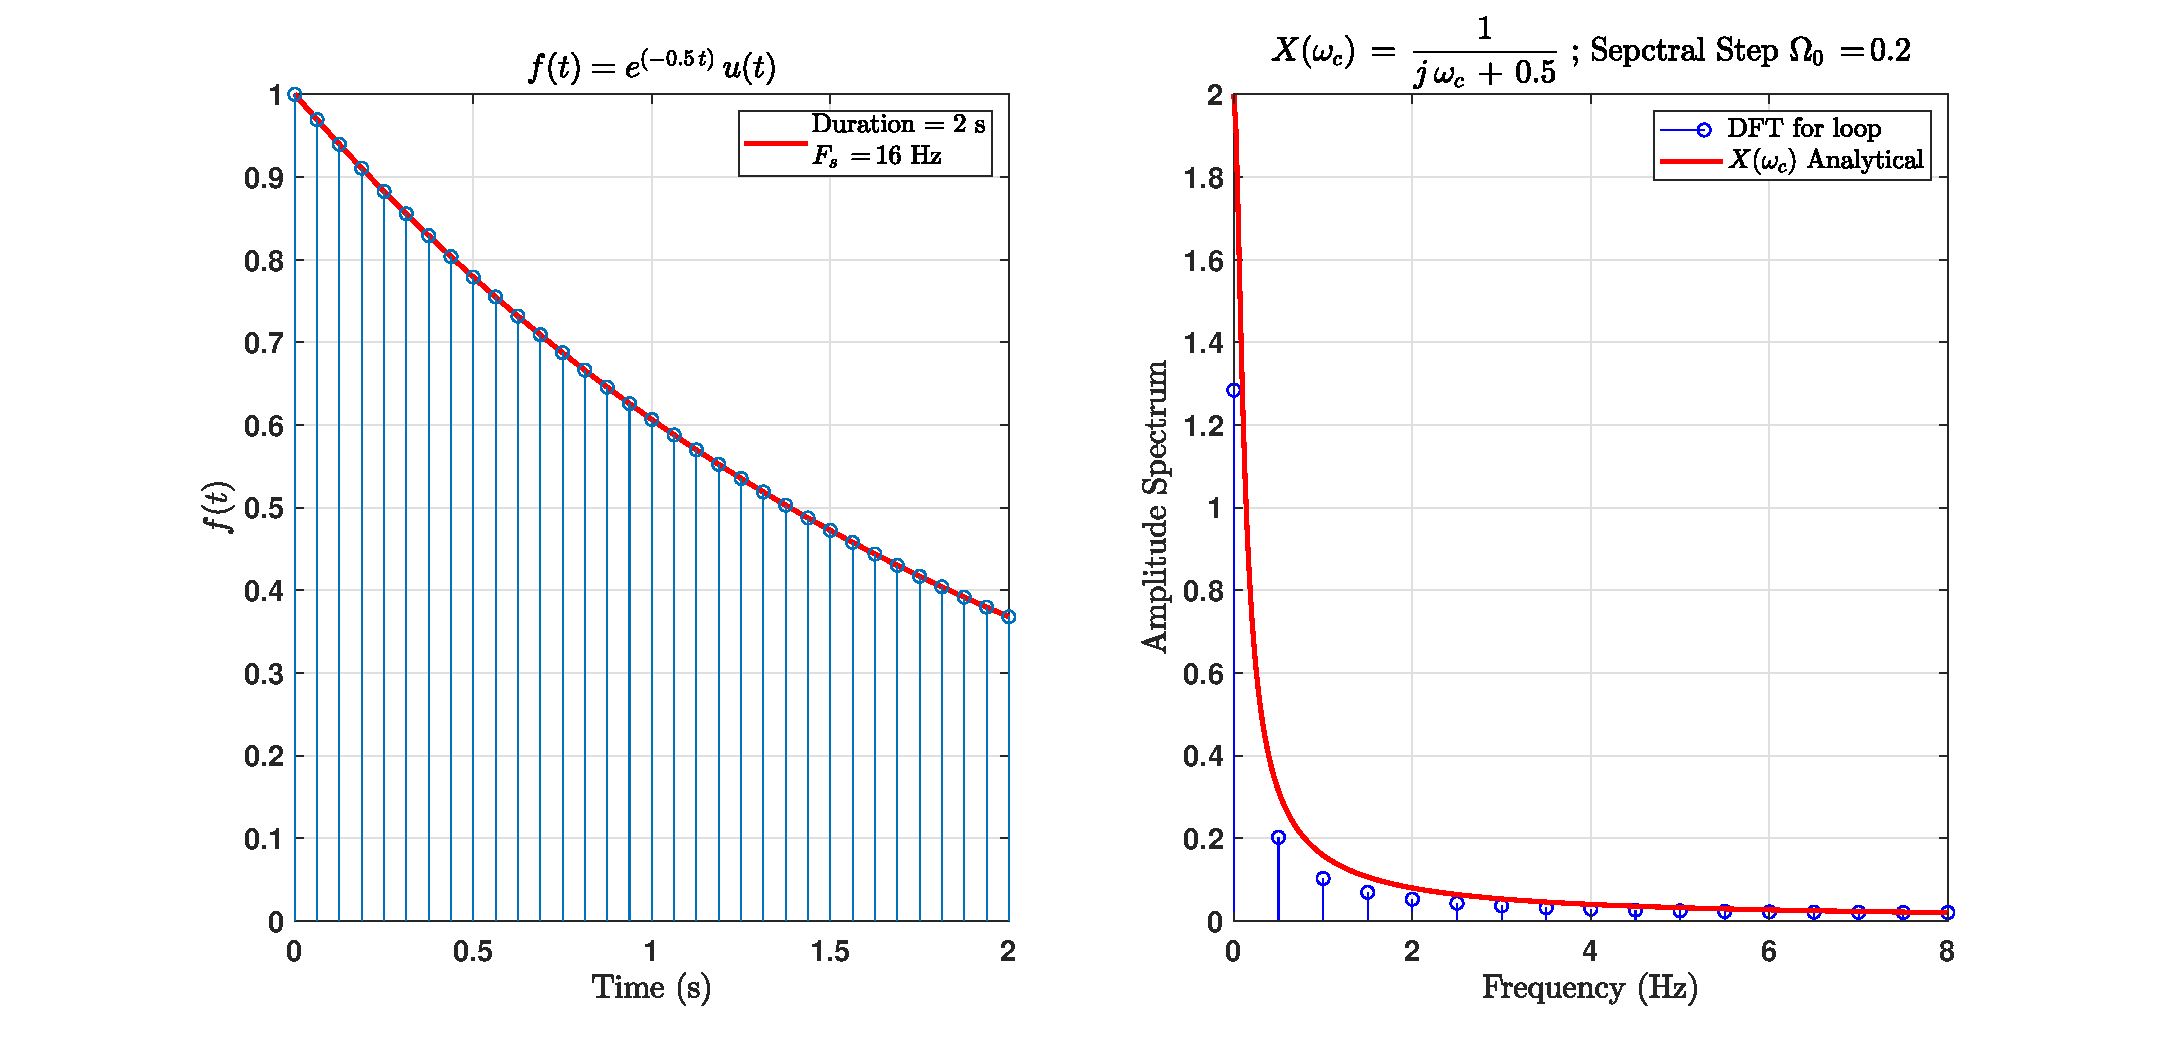
\includegraphics[scale = 0.30]{Figures/DFT/DFT_CTFT_duration_2}
\label{fig:Simulation_Sampling_Frequency_Analysis:DFT_CTFT_2}
\caption{ \textcolor{red}{Truncation in time} to 2 s duration}
\end{figure}

\begin{itemize}

\item \textcolor{red}{Dropping down the time window} of the signal from $16$ s $\rightarrow$ 2 s:

	\begin{itemize}

\item Although that $F_s \, = \, 16$ Hz, the DFT values didn't have exact values for the lower frequency part as in the close form formula

\item \textcolor{red}{Even} if we have a \textcolor{red}{good choice for $F_s$} but we truncate allot in time, we may have a \textcolor{red}{distortion for the DFT values}
	
	\end{itemize}


\end{itemize}


\newpage
\begin{figure}[h]
\centering
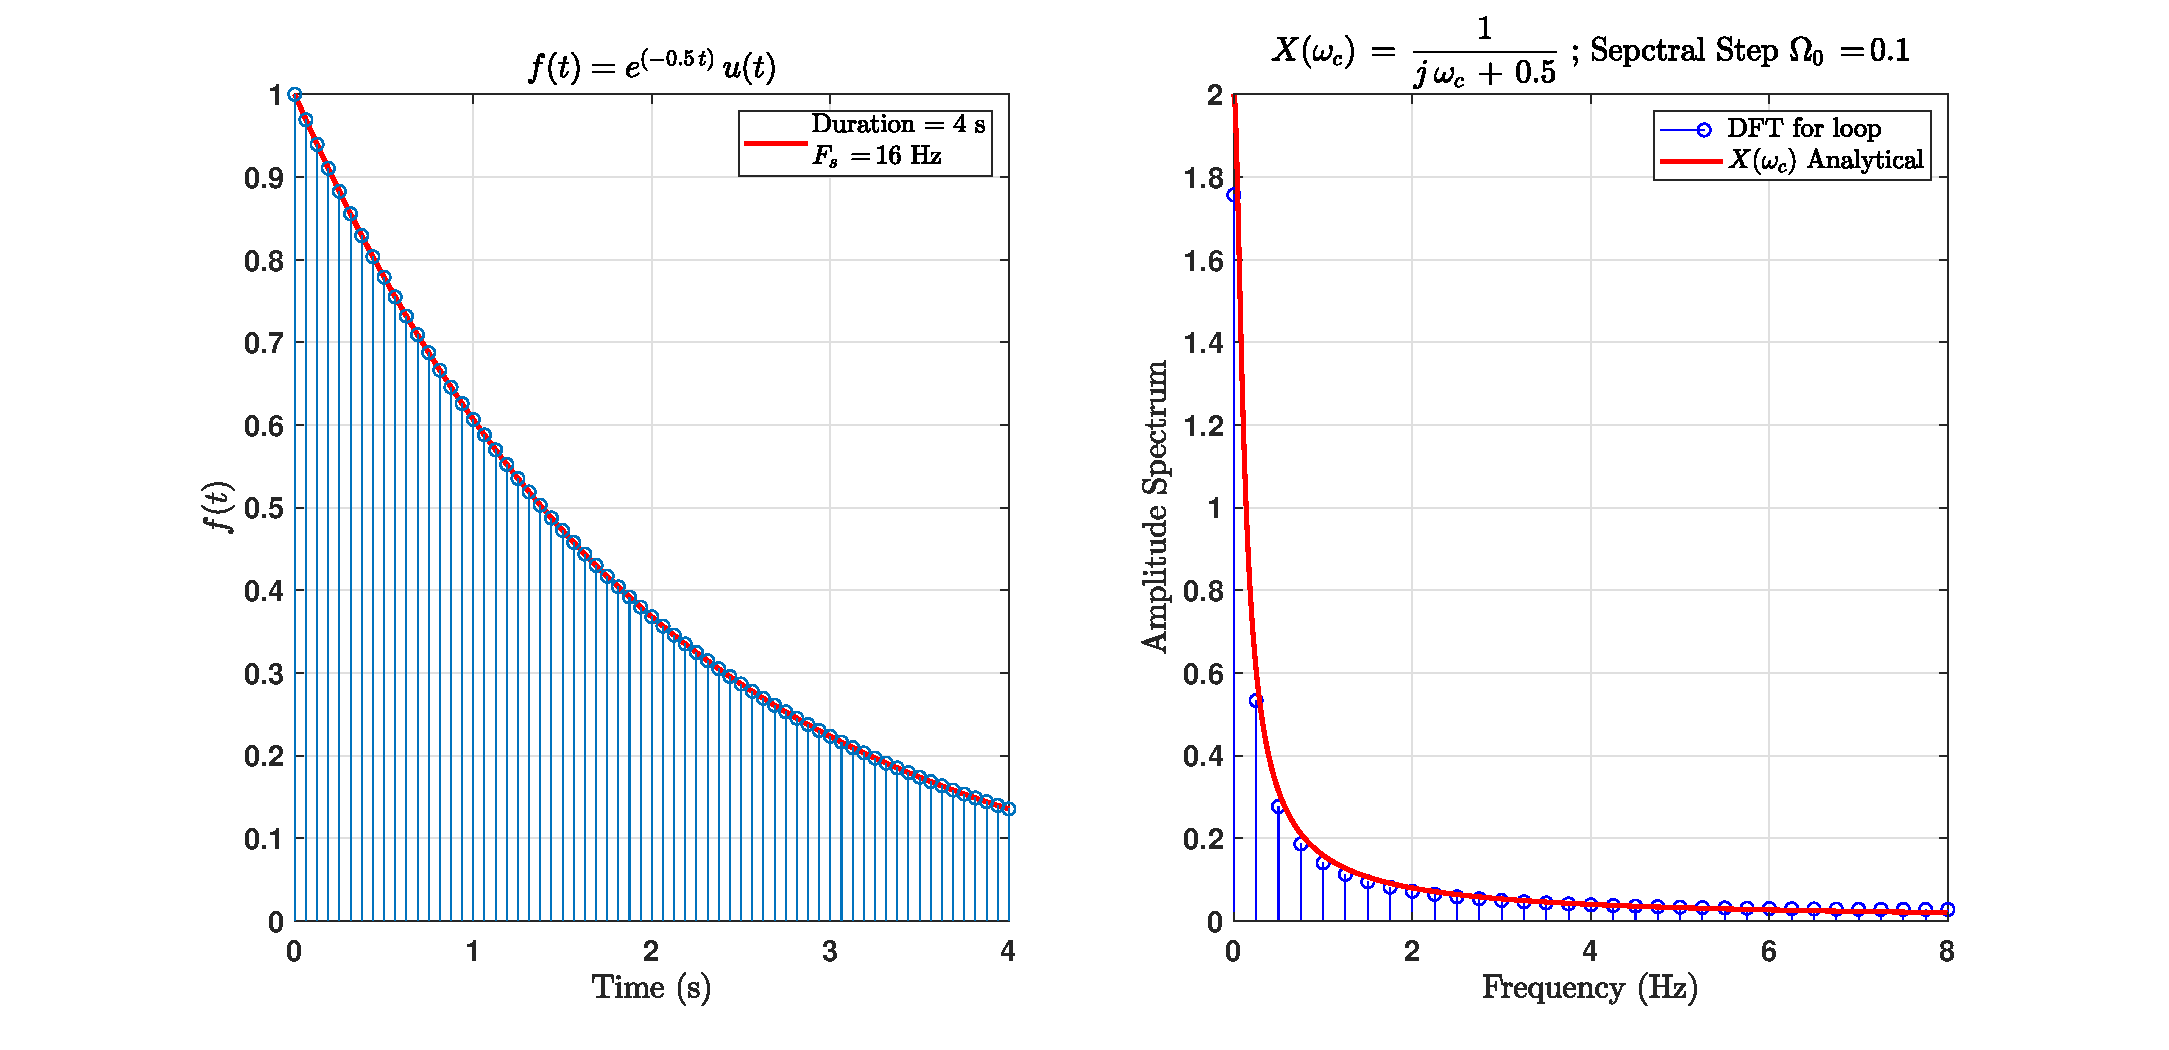
\includegraphics[scale = 0.3]{Figures/DFT/DFT_CTFT_duration_4}
\label{fig:Simulation_Sampling_Frequency_Analysis:DFT_CTFT_4}
\caption{Now we truncating less: increasing window size from 2 s $\rightarrow$ 4 s}
\end{figure}

\begin{itemize}

\item Truncating less $\rightarrow$ DFT values is getting more accurate

\end{itemize}

\end{frame}

\subsubsection{Some Practical Notes Regarding Programming}

\begin{frame}[t,fragile,allowframebreaks]{Practical Notes and Mistakes}

\begin{enumerate}

\item Frequency Variables $\omega_c$ in rad and $f_c$ in Hz:

	\begin{itemize}
	\item The Fourier transform of the signal $x(t) \, = \, \text{exp}(-0.5 \, t) \, u(t)$ can be written in function of $\omega_c$ or $f_c$: $  X(\omega_c) \, = \, \displaystyle\frac{1}{j \, \omega_c\, + \, 0.5} \, = \, \displaystyle\frac{1}{j \, 2 \,\pi \,f_c\, + \, 0.5}$ 
	
	\item However, whether we choose the variables  $\omega_c$ or $f_c$, the \textcolor{red}{values of the amplitude spectrum remain the same}
	
		\begin{itemize}
		\item $\displaystyle\left\lvert X(\omega_c) \displaystyle\right\rvert \, = \, \displaystyle\left\lvert X(f_c) \displaystyle\right\rvert$
		\end{itemize}
	\end{itemize}

\newpage
\item Frequency vector (bins)

	\begin{itemize}
	\item Analyticaly continuous frequency vector: from $0 \, \rightarrow \, \displaystyle\frac{F_s}{2} \, \leftrightarrow \,$ \verb|linespace(0,fs/2, nb_point)| where \verb|nb_point = | $\displaystyle\frac{\text{Signal Duration}}{\text{Sampling Period}}$
	
	\item Transform from $\omega_c \rightarrow \, f_c$: 
	
	\begin{itemize}
	\item $\omega_c \, = \, $ \verb|linespace(0,2 * pi* fs/2, nb_point)|
	
	\item In math, $f_c \, = \, \displaystyle\frac{\omega_c}{2 \pi}$ \textcolor{red}{but in programming}: \verb|fc = wc/(2*pi)| $\leftrightarrow$ \textcolor{red}{don't forget the ()}
	
	\end{itemize}		
	
\item Numerical Frequency Bins in Hz: \verb|freq_vector_fft =| 
\verb|linspace(-fs/2,fs/2 - freq_step,length_fft)| where 
\verb|freq_step = fs/length_fft| and \verb|length_fft = 2^nextpow2(nb_of_point)|

    \begin{itemize}
        \item Discrete Frequency in rad:
        \verb|discrete_freq_vector_fft =  (freq_vector_fft).*(2*pi)./fs| used in \verb|DTFT_FFT|
    \end{itemize}

	
	\end{itemize}



\end{enumerate}

\end{frame}

\subsubsection{Scaling Frequency bins}

\begin{frame}[t,allowframebreaks]{Scaling from DFT bins}

\begin{figure}[h]
\centering
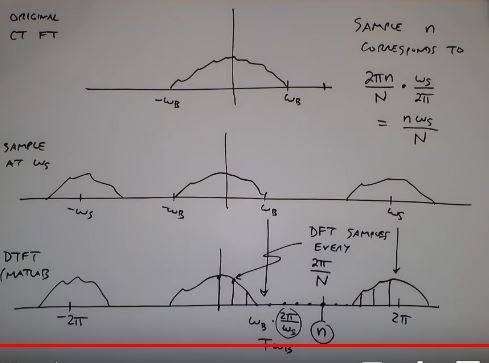
\includegraphics[scale = 0.5]{Figures/DFT/scaling_freq_bins}
\label{fig:DFT:scaling_freq_bins}
\end{figure}


\newpage

\begin{itemize}

\item $\displaystyle\frac{2 \pi}{N}$ is the DFT frequency step

\item $\displaystyle\frac{2 \pi}{N} \, \times \, n$ is the $n^{th}$ sample DFT bin

\item To convert back in  frequency bin in Hz: $\displaystyle\frac{n \, \omega_s}{N}$

\end{itemize}

\end{frame}

\subsection{DFT for DTFT on Finite Duration Signal}

\subsubsection{Given}
\begin{frame}[t,allowframebreaks]{Given}

\begin{itemize}

\item Consider a finite length sequence $x[k] \, = \, \{3,2,3\}$ where $N_o \, = 3$ and $\Omega_o \, = \, \displaystyle\frac{2 \pi}{3}$


\item DTFT of $x[k]$ is $X(\omega_d) \, = \, e^{-j \omega_d} \, \left[ \, 6 \, \text{cos}(\omega_d) \, + \, 2  \,\right]$

\item Computation:

\begin{equation*}
\begin{array}{rcl}
X(\omega_d) \, &=& \, \displaystyle\sum_{k \, = \, - \infty}^{+ \infty} x[k] \, \text{exp} \left( \,-j \, \omega_d \, k  \,\right) \\ \\
&=& \, \displaystyle\sum_{k \, = \, 0}^{+ 3} x[k] \, \text{exp} \left( \,-j \, \omega_d \, k  \,\right) \\ \\

&=& \, \text{exp} \left( \,-j \, \omega_d \, k  \,\right) \left[ \, 3 \, e^{j \omega_d} \, + \, 2  \, + \, 3 \,  e^{-j \omega_d} \,\right] \\ \\
&=& \, \text{exp} \left( \,-j \, \omega_d \, k  \,\right) \left[ 6 \, \text{cos }\omega_d \, + \, 2 \,\right]
\end{array}
\end{equation*}


\item We test in the following slides effect of the zero padding on DFT spectrum for DTFT

\end{itemize}

\end{frame}


\subsubsection{Results}
\begin{frame}[t,allowframebreaks]{Results}

\begin{figure}[h]
\centering
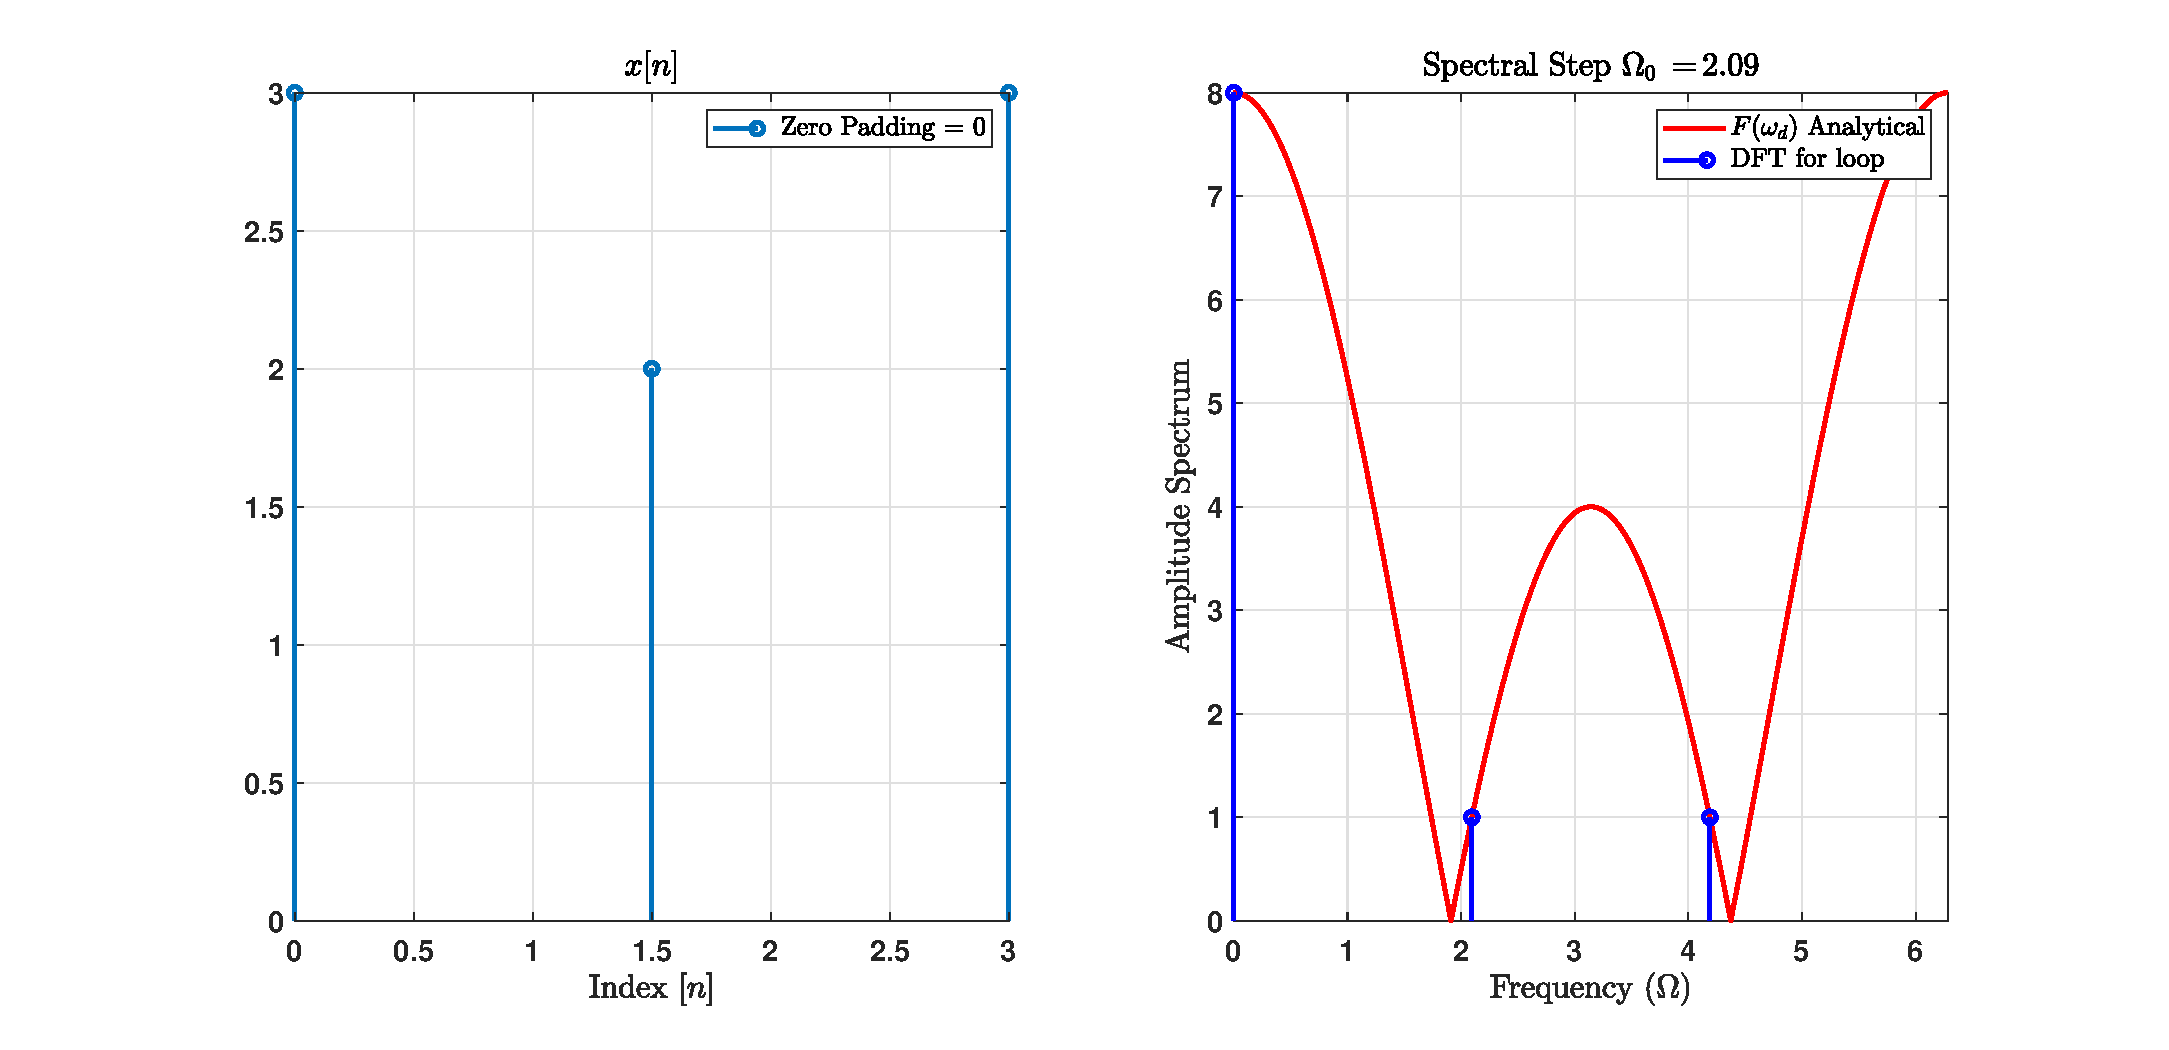
\includegraphics[scale = 0.25]{Figures/DFT/DFT_DTFT_zero_padd_0}
\label{fig:DFT:DTFT_zero_padd_0}
\end{figure}

\begin{itemize}
\item No Padding at all: the DFT of the DTFT only capture the essential information

\item However the plot doesn't look the same yet as the closed form
\end{itemize}

\begin{figure}[h]
\centering
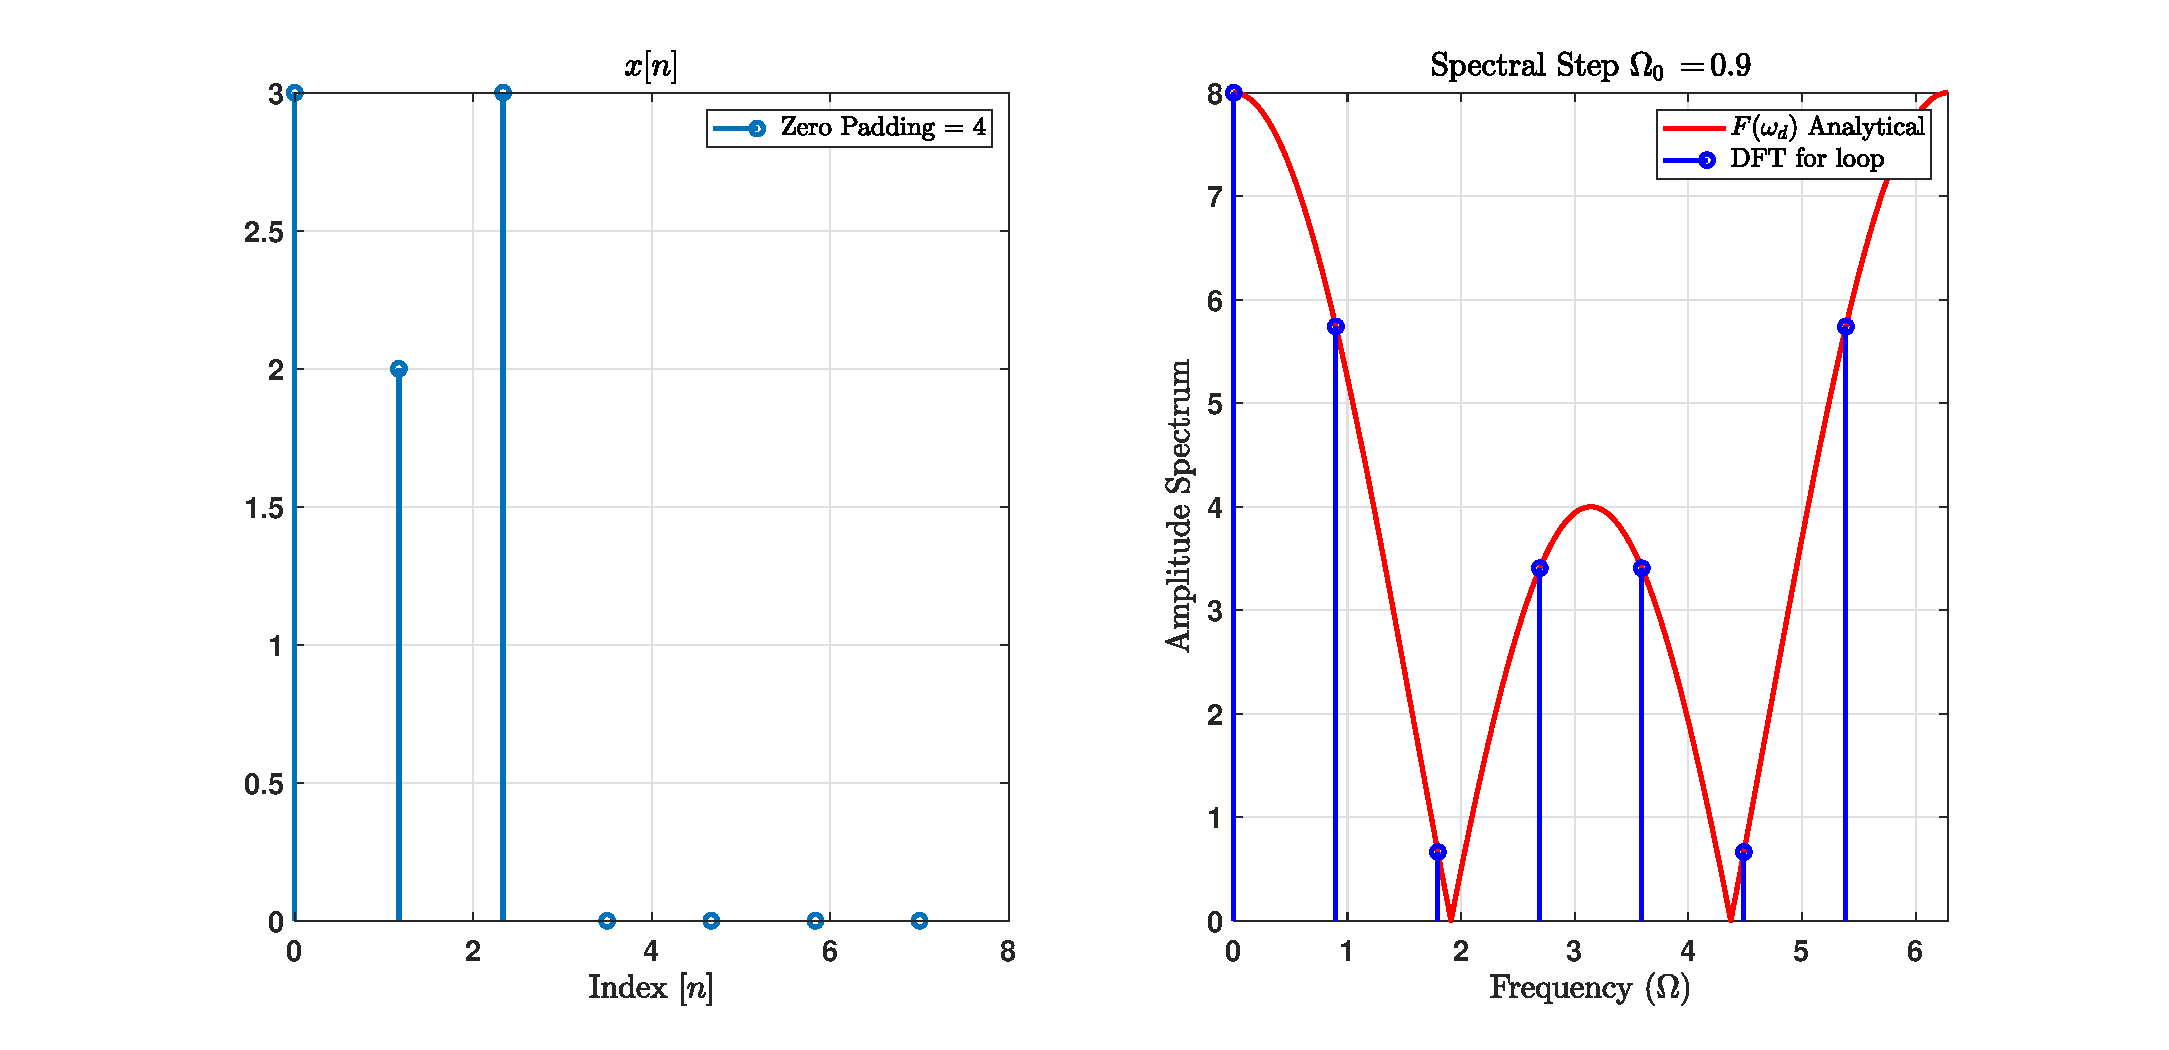
\includegraphics[width = 0.7\textwidth]{Figures/DFT/DFT_DTFT_zero_padd_4}
\caption{Padd more zeros make the spectrum more dense}
\label{fig:DFT:DTFT_zero_padd_4}
\end{figure}

\end{frame}


\subsection{Window Analysis}


\subsubsection{Introduction}
\begin{frame}[t,allowframebreaks]{Introduction}

\underline{\textcolor{purple}{References}:} based on section 7.6 in \cite{DSP_DimitrisManolakis} and section 4.9 in \cite{signal_processing_Lathi}

\begin{itemize}

\item As we have seen, DFT (or FFT) are the computational tools which can approximate any type of Fourier transform (CTFT, CTFS,$\cdots$)

\item The problem of computing the DFT is always done by passing through 3 fundamental steps

	\begin{enumerate}
	\item sample the continuous-time signal
	
	\item select a finite number of samples for analysis
	
	\item compute the spectrum at a finite
number of frequencies (frequency sampling)
	\end{enumerate}


\item Truncation is always done in real time signal processing since we have a limited amount of memory to store and process signals

\newpage
\item Focus in this section:effects of the \textcolor{red}{selection of a finite-length segment of the sampled signals}, because it
has the biggest impact on the accuracy of the estimated spectrum.

	\begin{itemize}
	\item In other words:  analysis of truncation and \textcolor{red}{window choice} in the spectrum
	\end{itemize}


\item We assume also that the signal is sampled correctly in the time domain
	\begin{itemize}
	\item Effects of aliasing are negligible 
	\end{itemize}

\end{itemize}

\end{frame}

\subsubsection{Modeling the problem of truncation}
\begin{frame}[t,allowframebreaks]{Modeling the problem of truncation}

\begin{itemize}

\item Selecting a finite number of samples in the signal $\leftrightarrow$ multiplying the signal with some window

\item Multiplying in the time domain $\leftrightarrow$ convolution in the frequency domain

\item We consider first a \textcolor{red}{rectangular window using simple cos signals}, then make the analysis for other choices


\item Mathematical equations:

\begin{equation}
\begin{array}{rcl}
f_w(t) \, = \, f(t) \, \times \, w(t) \leftrightarrow \, F_w(\omega_c) \, = \, F(\omega_c) \, * \, W(\omega_c)
\end{array}
\end{equation}

\newpage
\item Analysis by inspection: if we take $\text{rect} \left(\, \displaystyle\frac{t}{\text{duration}} \,\right) \, \leftrightarrow \, \text{sinc} \left(\,\displaystyle\frac{\omega_c \, \times \, \text{duration}}{2} \, \right)$

	\begin{itemize}
	\item Main lobe width $= \, \displaystyle\frac{4 \pi}{\text{duration}}$ (see figure \autoref{fig:DFT:amp_spec_rect_window})
	
	\item Convolution of 2 signals: shifting and adding the 2 signals up
	
	\item So if we have some frequency content in our signal, it will be added up (\textcolor{red}{signal will be blurred}) in the main lobe of the sinc
	\end{itemize}


\newpage
\begin{figure}[h]
\centering
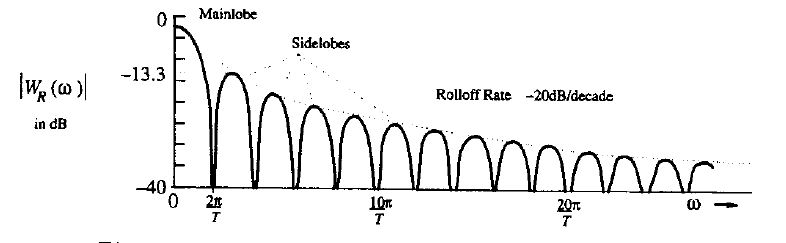
\includegraphics[scale=0.4]{Figures/DFT/amp_spec_rect_window}
\caption{Amplitude Spectrum for Rectangular Window \cite{signal_processing_Lathi}}
\label{fig:DFT:amp_spec_rect_window}
\end{figure}



\end{itemize}

\end{frame}



\begin{frame}[t,allowframebreaks]{Computations for a Cos Signal}

\begin{itemize}

\item Let $x_c(t) \, = \, A_1 \, \cos(\omega_c \, t \, + \, \phi)$

\item The spectrum of $x_c(t)$ can be directly obtained using Euler identity

\begin{equation}
    x_c(t) \, = \, \displaystyle\frac{1}{2} \, A_1 \, e^{-j \, \phi} \, e^{-j \, \omega_c \, t} \, + \, \displaystyle\frac{1}{2} \, A_1 \, e^{j \, \phi} \, e^{j \, \omega_c \, t}
\end{equation}


\item The time windowed signal $x_w(t)$:

\begin{equation}
 x_w(t) \, = \, \displaystyle\frac{1}{2} \, A_1 \, e^{-j \, \phi} \, w_c(t) \, e^{-j \, \omega_c \, t} \, + \, \displaystyle\frac{1}{2} \, A_1 \, e^{j \, \phi} \, \, w_c(t) \, e^{j \, \omega_c \, t} 
 \label{Eq:DTF:Window_Eq_1}
\end{equation}

\item Taking the CTFT of \autoref{Eq:DTF:Window_Eq_1} and using the frequency shift property \cite{signal_processing_Lathi} ( $f(t) \, e^{j \, \omega_0 \, t} \leftrightarrow \, F(\omega_c \, - \, \omega_0)$ ), we have:

\begin{equation}
   X_w(\omega_c) \, = \, \displaystyle\frac{1}{2} \, A_1 \, e^{-j \, \phi} \, W_c(\, \omega_c \, + \, \omega_0 \,)  \, + \, \displaystyle\frac{1}{2} \, A_1 \, e^{j \, \phi} \, \, W_c(\, \omega_c \, - \, \omega_0 \,)
 \label{Eq:DTF:Window_Eq_2}  
\end{equation}

\item Interpretation of \autoref{Eq:DTF:Window_Eq_2}: the effect of time windowing is to replace each spectral line of the CTFT spectrum with \textcolor{red}{scaled copy of}  $W_c(\omega_c)$ centered at the frequency  of the line

\item As an example of a window, we begin with a rectangular one 

\begin{equation}
\text{rect} \left(\, \displaystyle\frac{t}{\text{duration}} \,\right) \, \leftrightarrow \, \text{duration} \, \times \, \text{sinc} \left(\,\displaystyle\frac{\omega_c \, \times \, \text{duration}}{2} \, \right)    
\end{equation}

\end{itemize}

\end{frame}


\begin{frame}[t,allowframebreaks]{Recap of Windowing Effect Process \cite{DSP_DimitrisManolakis}}
 
\begin{figure}[h]
\centering
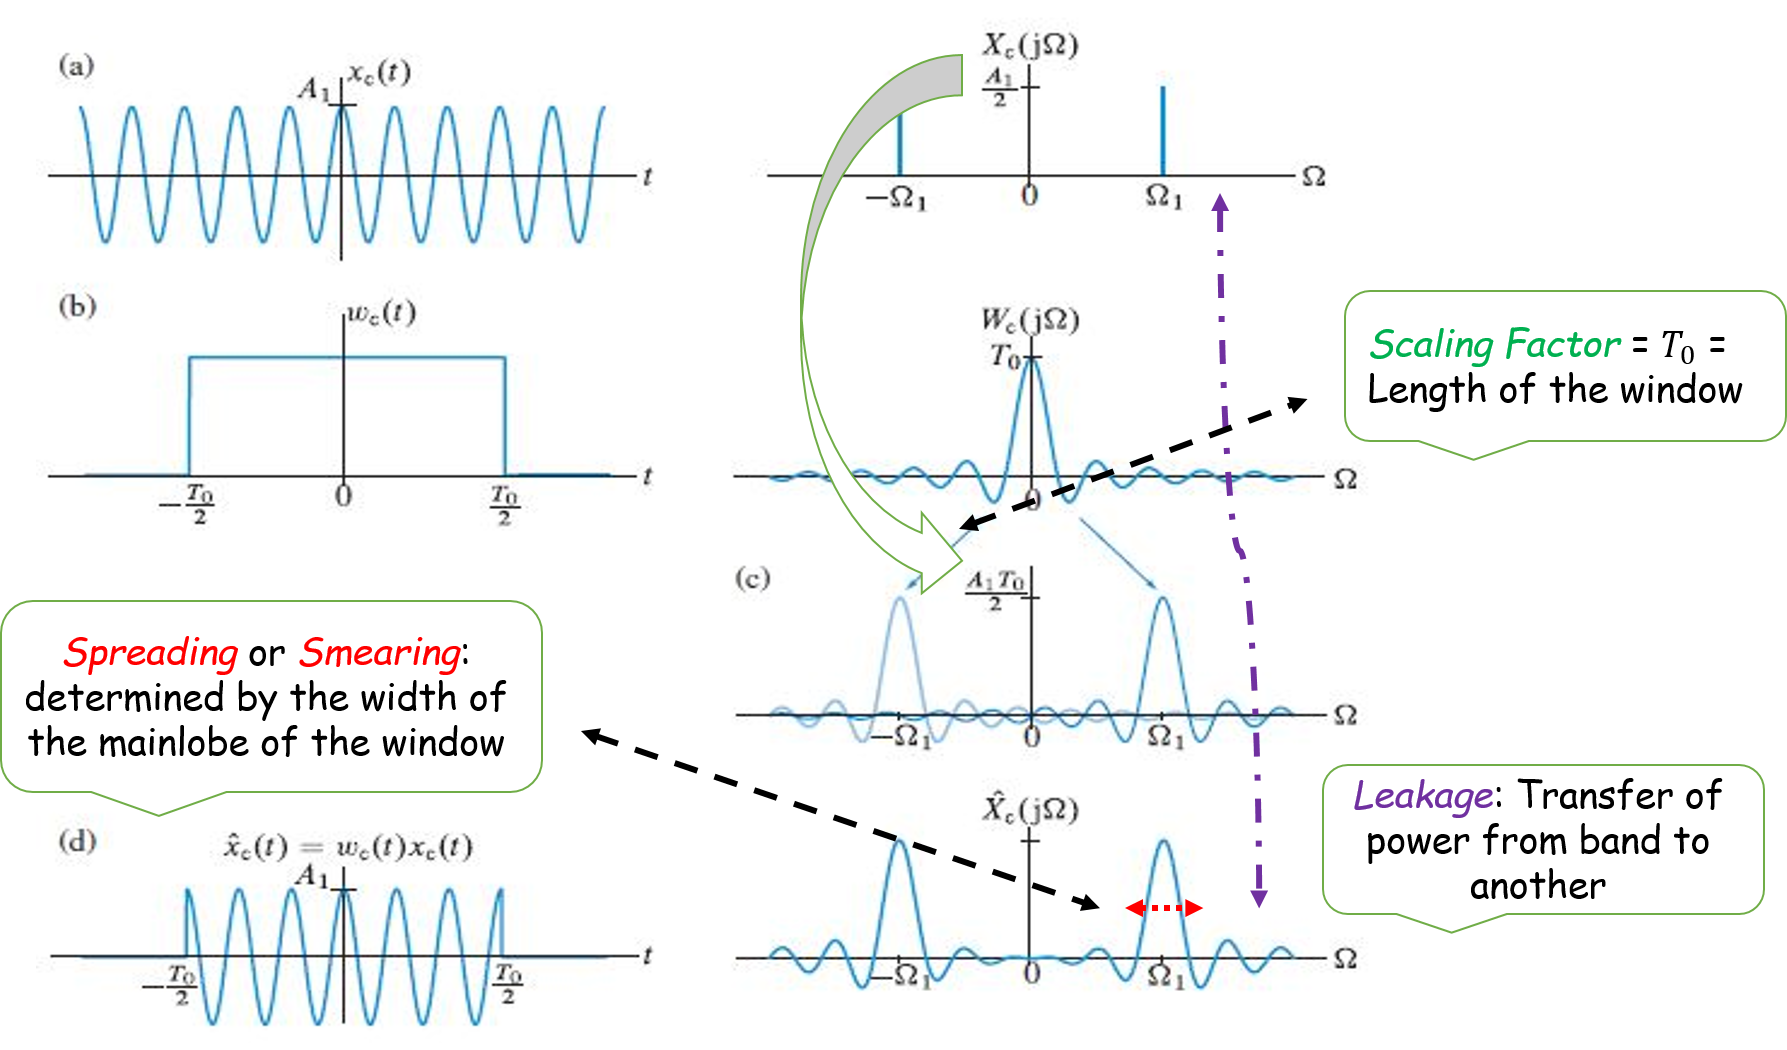
\includegraphics[width = 0.80\textwidth]{Figures/DFT/windowing_modeling_2}
\caption{Windowing Effect on CTFT Amplitude Spectrum}
\label{fig:DFT:windowing_modeling_2}
\end{figure}


3 Things to be noticed from figure \autoref{fig:DFT:windowing_modeling_2} \cite{DSP_DimitrisManolakis}

\begin{enumerate}

\item \textcolor{red}{Spectral Spreading} or \textcolor{red}{Spectral Smearing}

	\begin{itemize}
	
	\item Controlled by the \textcolor{red}{width of the main lobe}	
	
	\item The cosine signal now has spread out after and before $\omega_{c_1}$
	
	\item Smearing can cause \textcolor{red}{peak merging }$\leftrightarrow$ reduce the resolvability in the spectrum when have several components close to each other
	
		\begin{itemize}
		\item To be seen in the simulations after
		\end{itemize}
		
	\end{itemize}


\item \textcolor{red}{Leakage}:

	\begin{itemize}
	
	\item Controlled by the \textcolor{red}{sidelobs} of the rectangular window	
	
	\item Leakage create false peaks due to the power transfer
	
	\item Also it hides any weak frequency components as we will see in the simulation results after
	\end{itemize}


\item Also notice that the amplitude spectrum is multiplied by $T_0$, the length of the window

	\begin{itemize}
	\item This is because the rect window amplitude spectrum has a maximum equal to $T_0$
	\end{itemize}

\end{enumerate}



\end{frame}

\begin{frame}[t,allowframebreaks]{Truncation Effect for a Rectangular Window}

\begin{figure}[h]
\centering
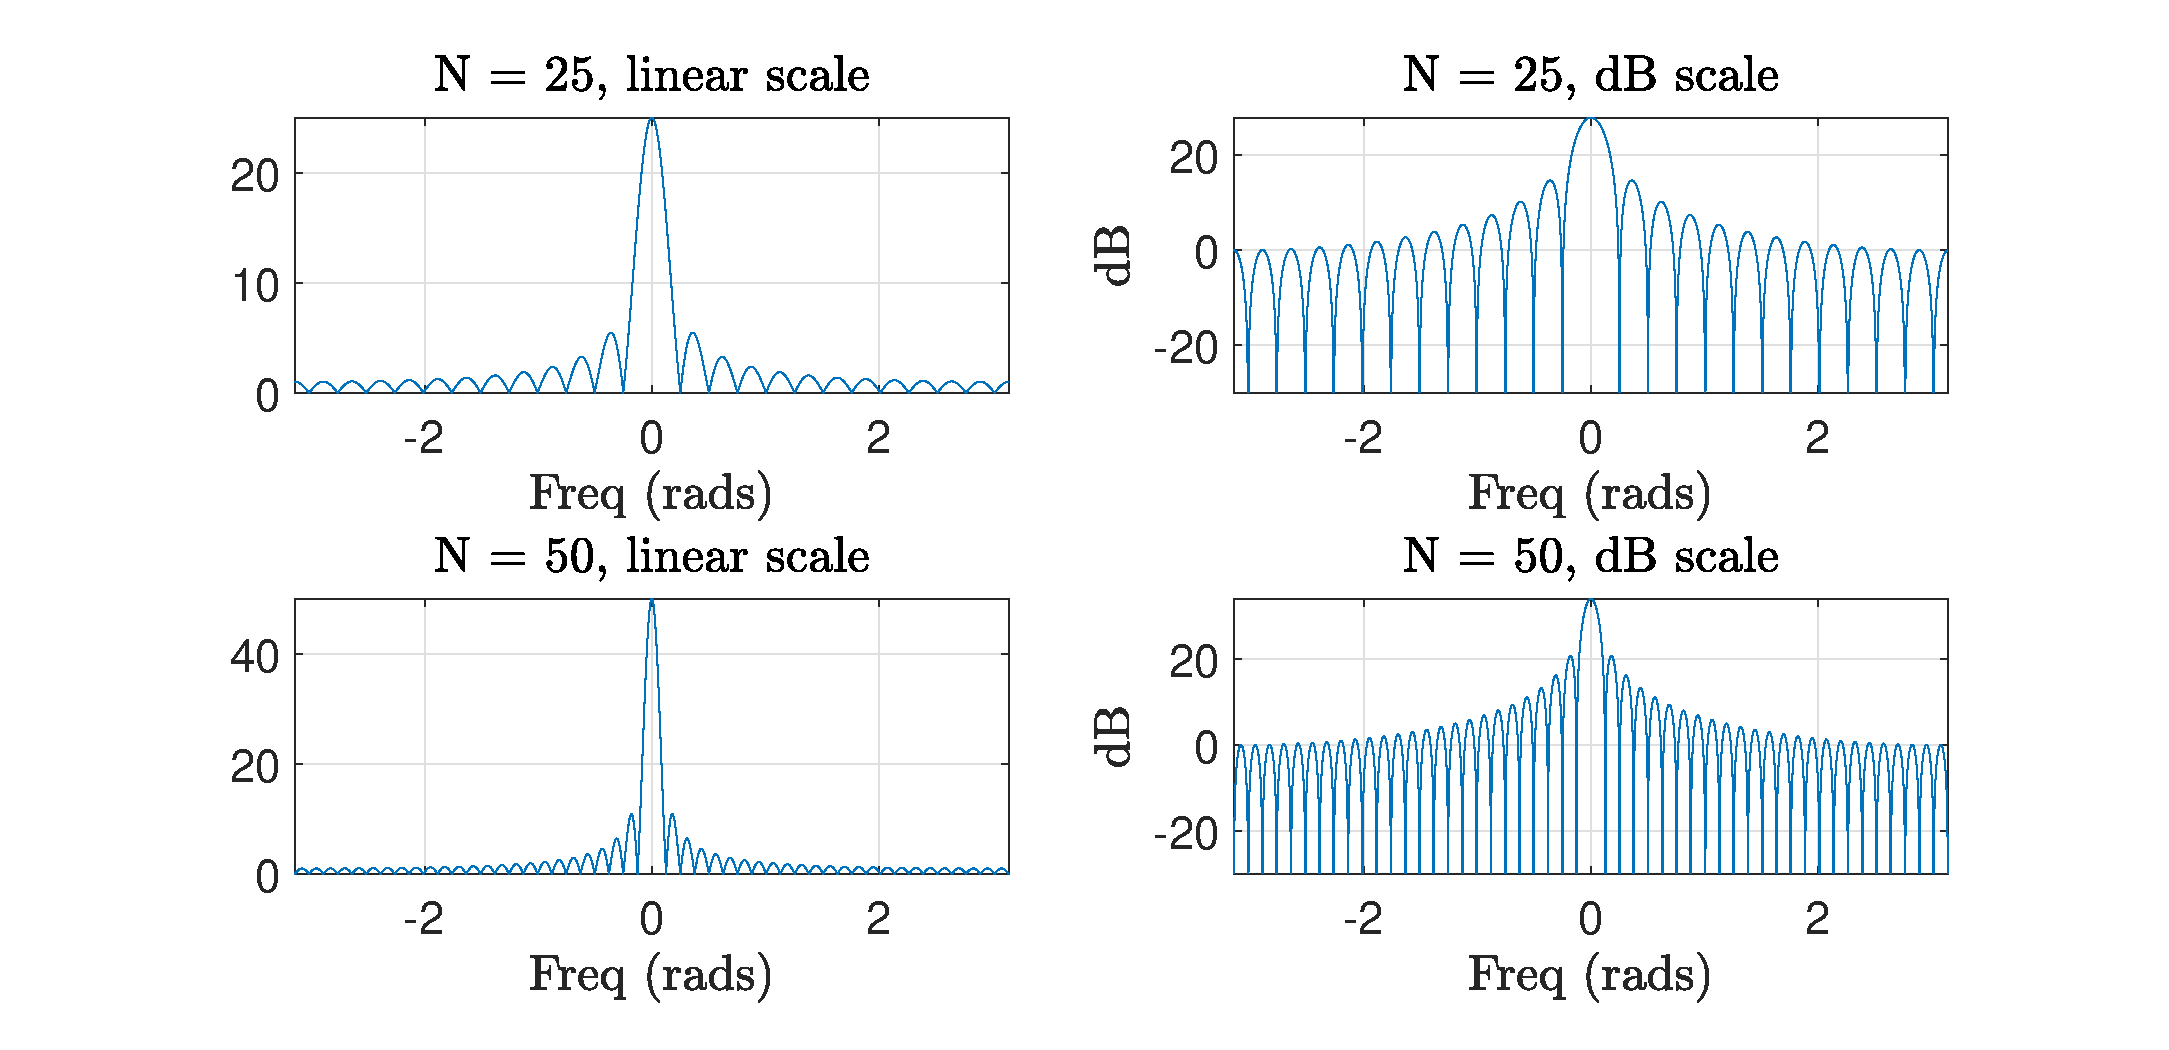
\includegraphics[scale = 0.3]{Figures/Simulation_Sampling_Frequency_Analysis/rect_window_nb_samples}
\caption{DTFT Amplitude Spectrum for the Rectangular Window in Linear and dB Scale}
\label{fig:Simulation_Sampling_Frequency_Analysis:rect_window_nb_samples}
\end{figure}

\begin{itemize}

\item What we can see is that if we choose \textcolor{red}{higher number of samples}


	\begin{enumerate}
	\item We get a \textcolor{red}{narrower main lobe}
	
	\item But the \textcolor{red}{side lobes doesn't change that much}
	\end{enumerate}

	
	\item If the \textcolor{red}{cosine signals are too close together}, then doing convolution with our window will add up the 2 cos, and hence we can't distinguish the frequency content of the signals
	
		\begin{itemize}
		\item This is known of \textcolor{red}{peak merging} (loss of spectral resolution) when the 2 spectral line are closer then the width of the main lobe \cite{DSP_DimitrisManolakis}
		\end{itemize}

\item In the next slides, we take several cases for 2 cos signals to illustrate more practically these ideas
	
\end{itemize}

\end{frame}


\subsubsection{Examples on Cos Signals}
\begin{frame}[t,allowframebreaks]{Examples of 2 Separated Cos signal}

\begin{figure}[h]
\centering
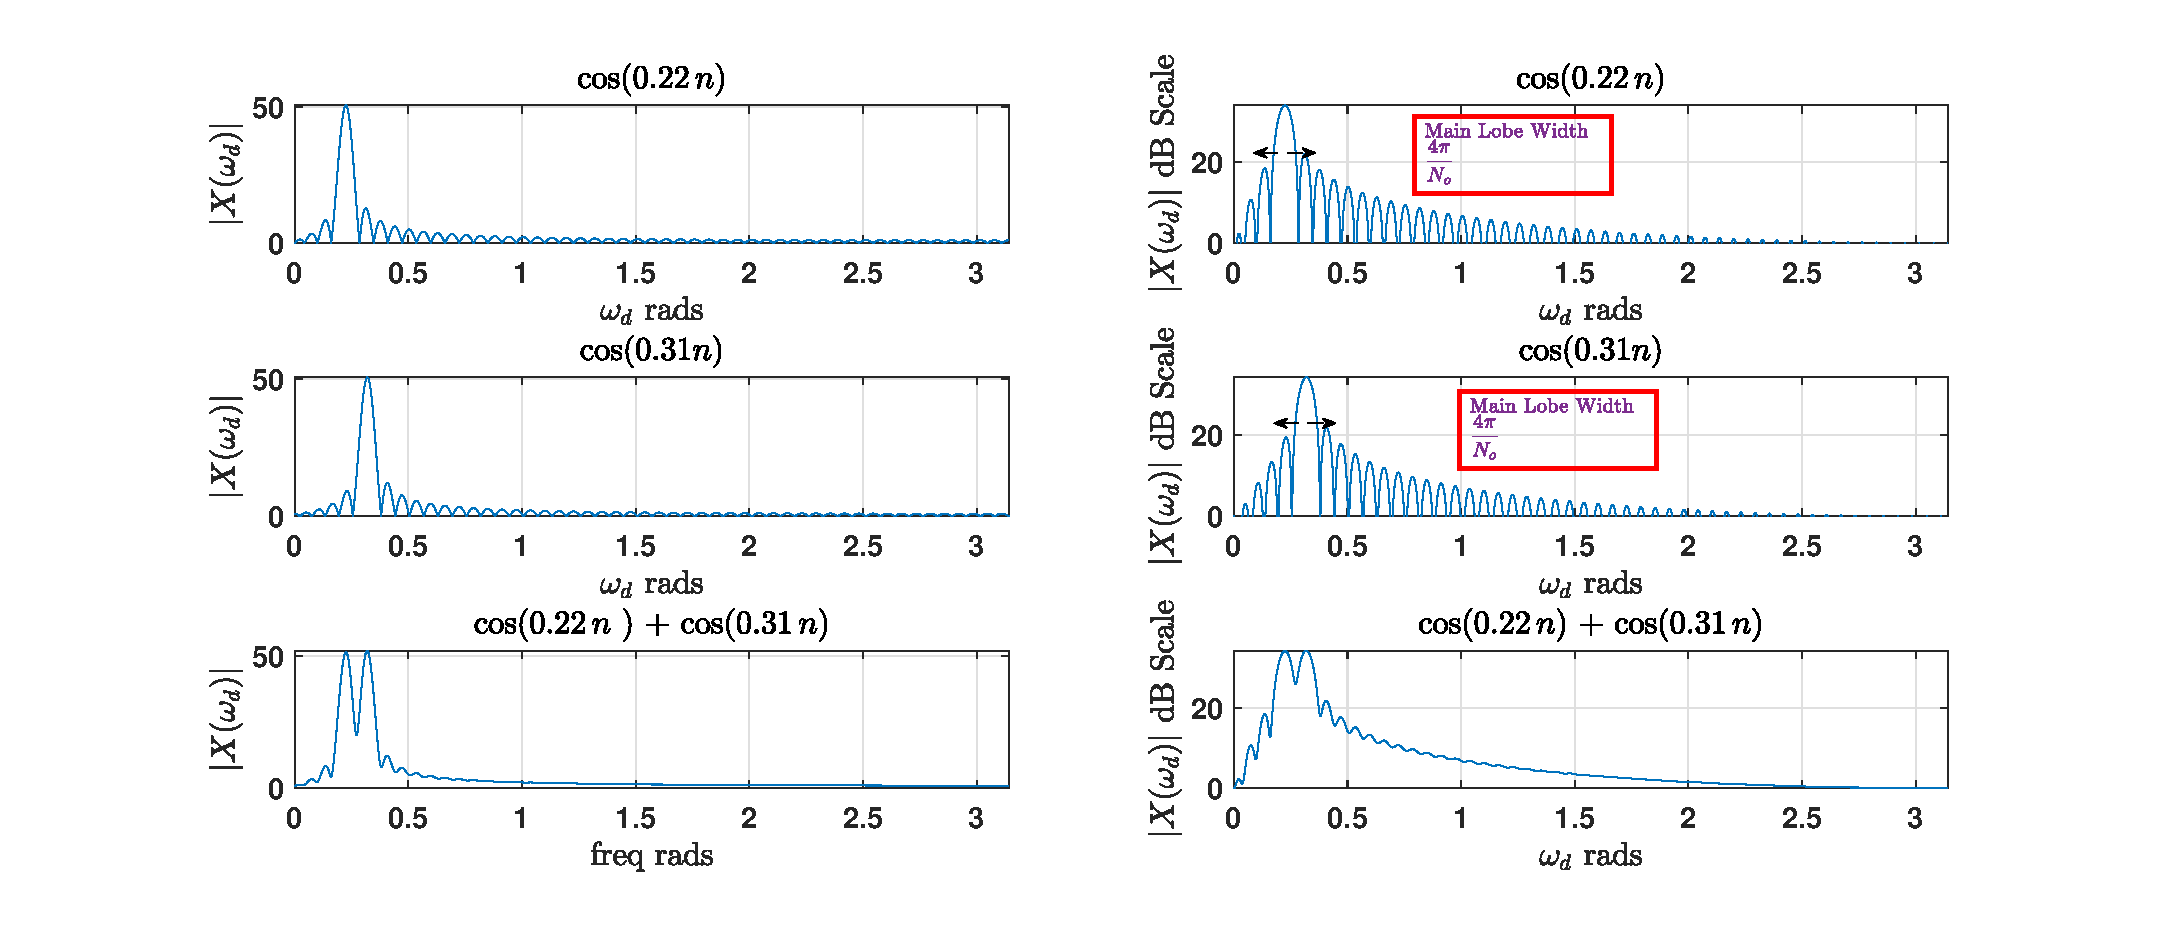
\includegraphics[width = 1\textwidth]{Figures/DFT/spaced_cos}
\caption{Spaced Cos signal}
\label{fig:DFT:spaced_cos}
\end{figure}

\newpage
\begin{itemize}

\item We have 2 cos signals with discrete frequencies:

	\begin{itemize}
	\item $ \omega_{d_1} \, = \, \displaystyle\frac{7 \pi}{100} \approx \, 0.22$ and $ \omega_{d_2} \, = \, \displaystyle\frac{10 \pi}{100} \approx \, 0.31$ 
	
	
	\end{itemize}

\item Width of the main lobe $ = \displaystyle\frac{4 \pi}{N} \, = \, \displaystyle\frac{4 \pi}{100}$

	\begin{itemize}
	\item Where $N$ is the length of the rectangular window
	\end{itemize}

\item Spectral separation between signals $= \displaystyle\frac{10 \pi}{100} \, - \, \displaystyle\frac{7 \pi}{100} \, = \, \displaystyle\frac{3 \pi}{100}$

\item Separation rule: Width of the main lobe $\leq$ Spectral separation between signals $\leftrightarrow \,\displaystyle\frac{4 \pi}{100} \,\leq \,  \displaystyle\frac{3 \pi}{100} \, \leftrightarrow$ rule is almost verified with some errors however

	\begin{itemize}
	\item  But still we are able to distinguish the 2 components
	\end{itemize}
	
\end{itemize}


\end{frame}

\begin{frame}[t,allowframebreaks]{Examples of 2 Close Cos signal}


\begin{figure}[h]
\centering
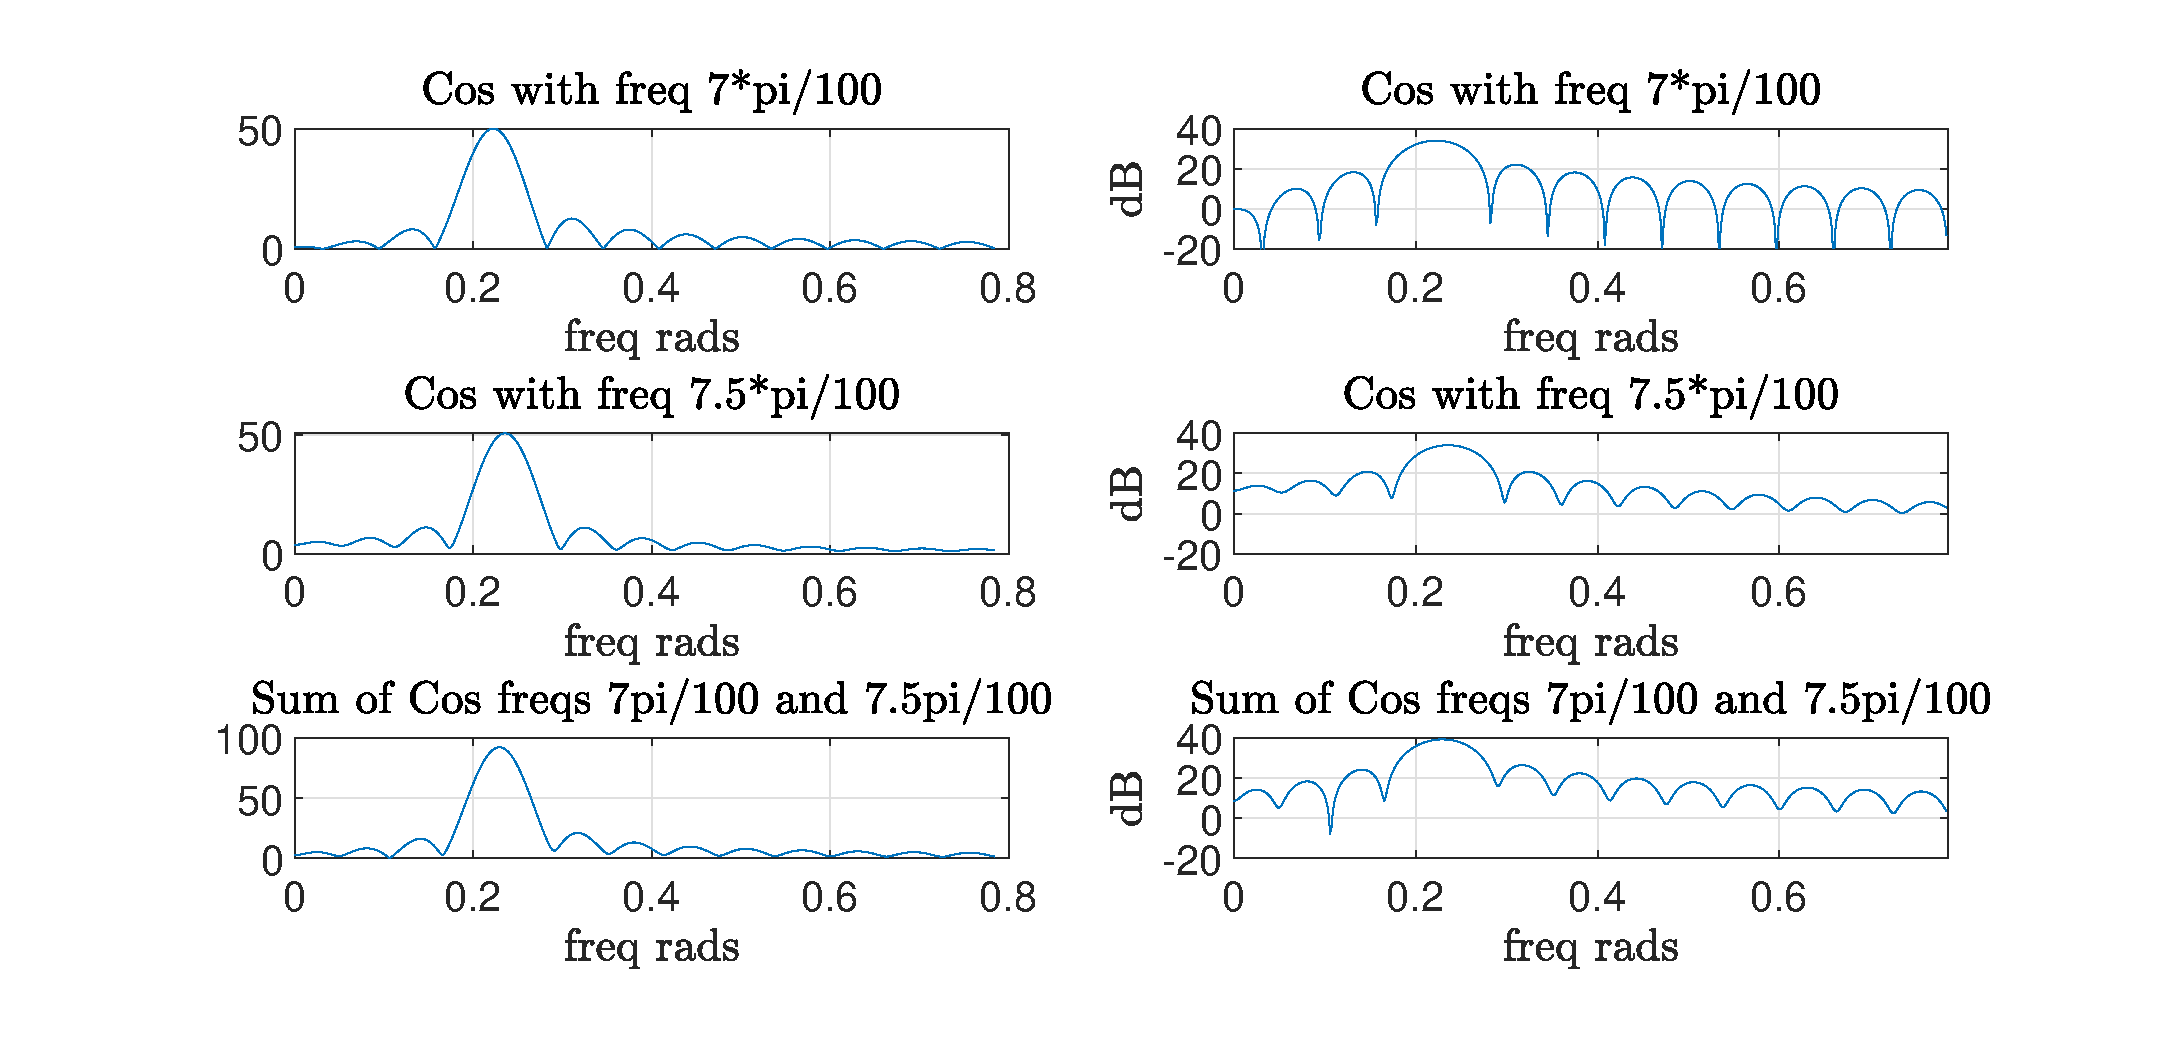
\includegraphics[width = 1\textwidth]{Figures/Simulation_Sampling_Frequency_Analysis/closed_cos}
\caption{Closed Cos signal: the components are added up $\leftrightarrow$ \textcolor{red}{peak merging}}
\label{fig:Simulation_Sampling_Frequency_Analysis:closed_cos}
\end{figure}

\end{frame}

\begin{frame}[t,allowframebreaks]{Examples of 1 Weak and 1 Strong}

\begin{itemize}
\item Trickiest part: don't forget \textcolor{red}{the side lobes}

	\begin{itemize}
	
	\item Case of 1 strong and the $\mathrm{2}^\mathrm{nd}$ is weak
	
	\item Even if the $\mathrm{2}^\mathrm{nd}$ component is far from the $\mathrm{1}^\mathrm{st}$ one, the $\mathrm{2}^\mathrm{nd}$ could be a small one and add up with the side lobes of the $\mathrm{1}^\mathrm{st}$ one (the strong one)
	\end{itemize}
	
\newpage
\begin{figure}[h]
\centering
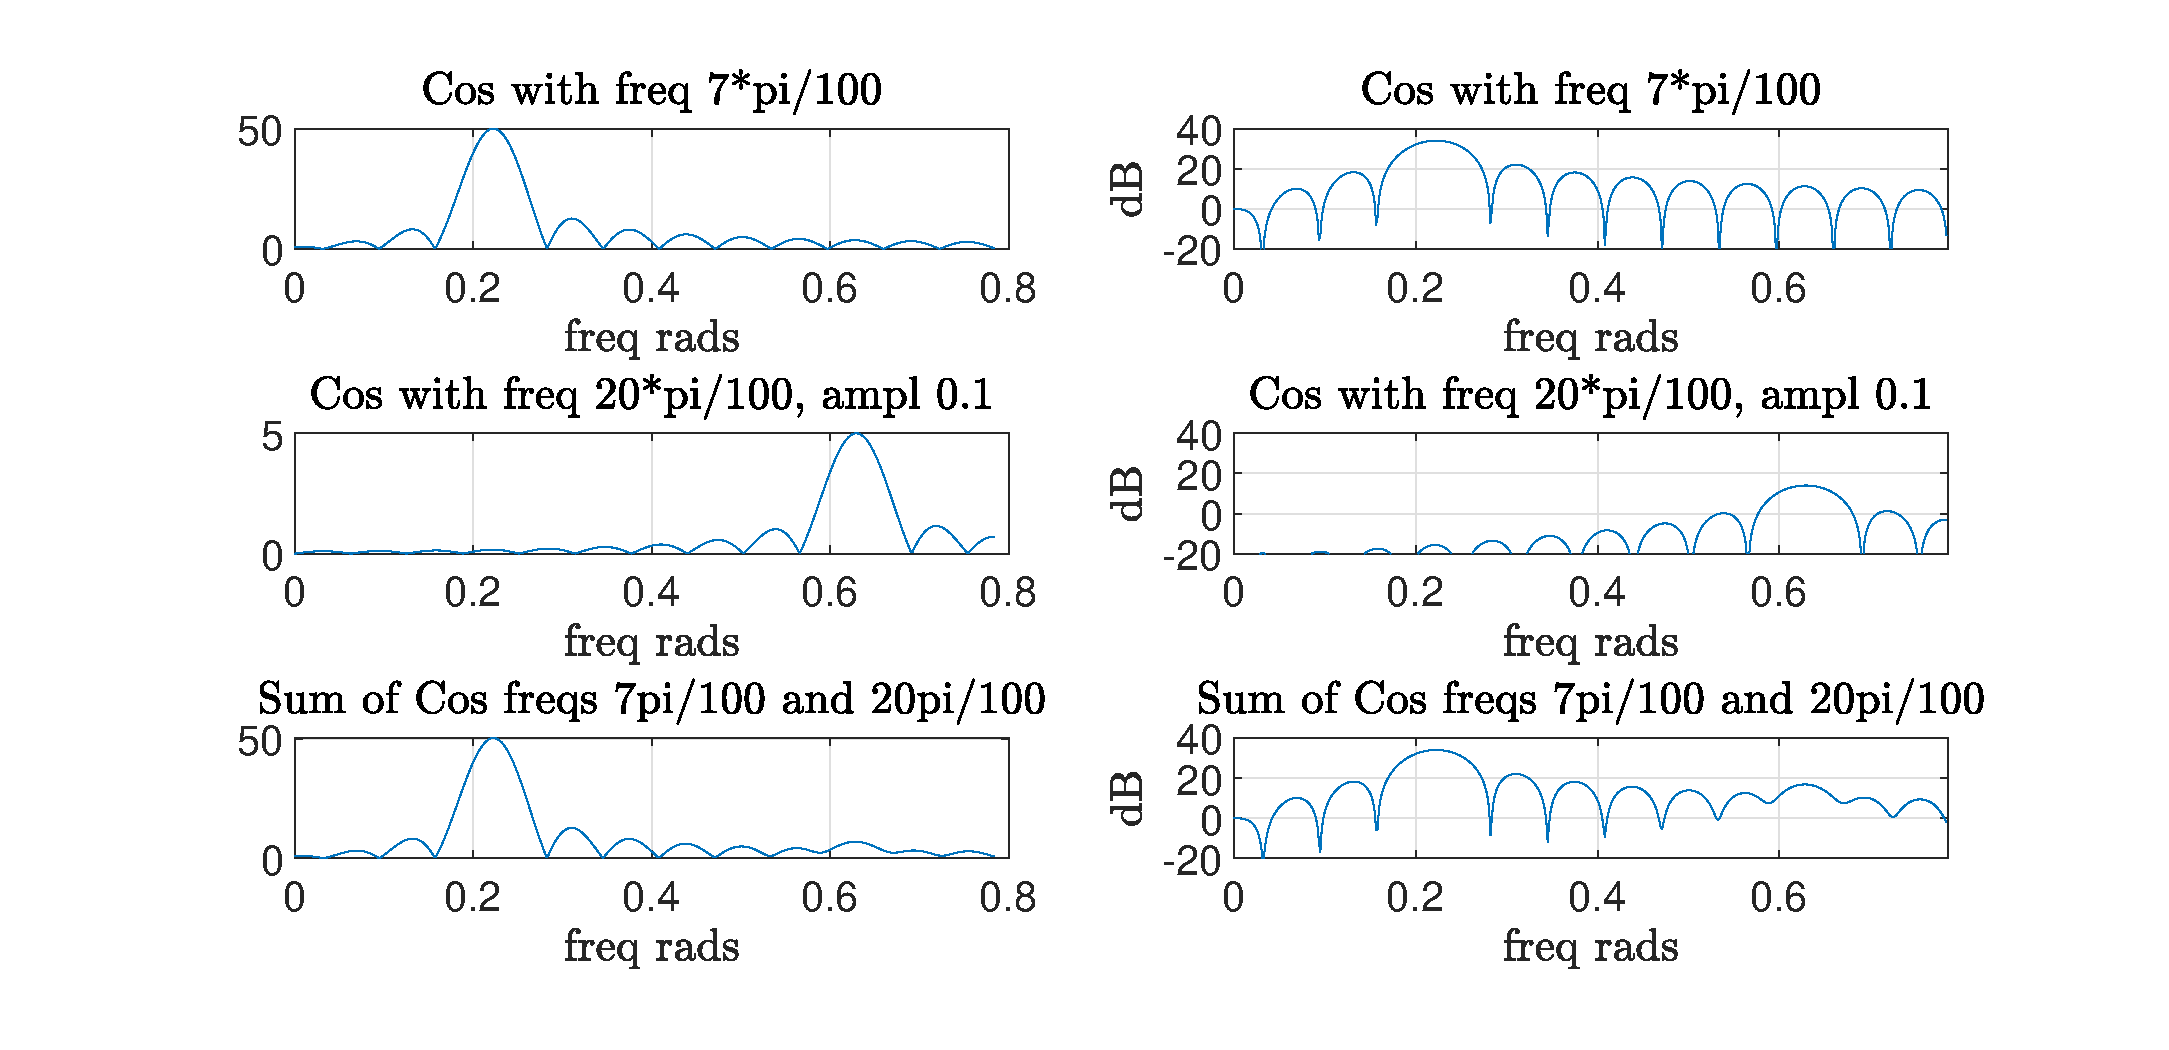
\includegraphics[width = 1\textwidth]{Figures/Simulation_Sampling_Frequency_Analysis/spaced_weak_cos}
\caption{Well separated signals but with weak components}
\label{fig:Simulation_Sampling_Frequency_Analysis:closed_cos}
\end{figure}

\end{itemize}


\end{frame}

\subsubsection{Window Choice}


\begin{frame}[t,allowframebreaks]{Windows Choice: Resolution vs Dyanamic Range}

\begin{itemize}

\item In previous part, we have seen the effect of side lobs in a rectangular window:

	\begin{enumerate}
	\item Very high resolution $\leftrightarrow$ narrow main lobe
	
	\item Not very efficient dynamic range $\leftrightarrow$ side lobe effects still high even if we truncate less
	\end{enumerate}


\item In rectangular window, we have a sudden transition from $1 \rightarrow 0$ or $0 \rightarrow 1$ in the time domain, which make the side lobes to be appear in the frequency domain (in CTFT or DTFT Spectrum)

\item This was the motivation for designing other choices of windows: \textcolor{red}{trade-off between resolution and dynamic range}

\item Design criteria for \textcolor{red}{good window}: 

	\begin{enumerate}
	\item Narrow mainlobe
	
	\item weak side lobes
	\end{enumerate}



\end{itemize}

\end{frame}

\begin{frame}[t,allowframebreaks]{Different Window Types}



\begin{figure}[h]
\centering
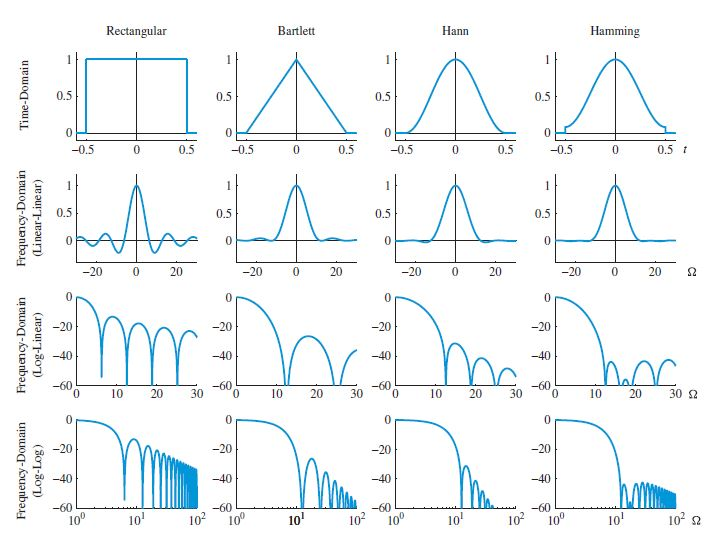
\includegraphics[scale=0.3]{Figures/DFT/other_windows}
\caption{Time-domain and frequency-domain characteristics of continuous-time rectangular, Bartlett (triangular), Hann, and Hamming windows \cite{DSP_DimitrisManolakis}}
\label{fig:DFT:other_windows}
\end{figure}


\begin{figure}[h]
\centering
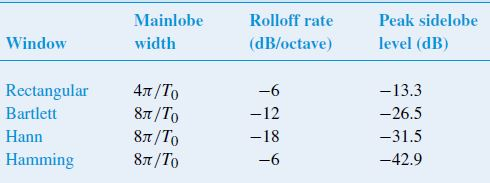
\includegraphics[scale=0.6]{Figures/DFT/other_windows_2}
\caption{Some continuous-time windows and their characteristics \cite{DSP_DimitrisManolakis}}
\label{fig:DFT:other_windows}
\end{figure}




\end{frame}


\begin{frame}[t,allowframebreaks]{Observation and Comparison Among Windows}

\begin{itemize}

\item Rectangular window has the narrower main lobe $\leftrightarrow$ highest resolution

	\begin{itemize}
	\item However, their side lobes are relatively high $\leftrightarrow$ poorest dynamic range
	\end{itemize}

\item Hamming window has a smoother transition in the time domain from $1 \rightarrow 0$

	\begin{itemize}
	\item Hence it has a wider mainlobe compared to the rectangular window $\leftrightarrow$ lower resolution
	
	\item But lower side lobes $\leftrightarrow$ higher dynamic range
	\end{itemize}

\newpage
\item Chebyscheve window: we can control the side lobes height, and it has equal height side lobes

	\begin{itemize}
	\item The weaker the side lobes the more the transition is smooth
	
	\item Chebychev with -30 dB attenuation: narrower main lobe but high side lobes
	
	\item Chebychev with -70 db has quite the opposite compared to the -30 dB attenuation
	\end{itemize}

\item As a general rule: the more we push down the side lobes in the frequency domain (hence better dynamic range) $\leftrightarrow$ the main lobe will get higher (lower resolution)

\end{itemize}

\end{frame}


\subsubsection{DTFT Spectrum Analysis using Different Windows}

\begin{frame}[t,allowframebreaks]{DTFT Spectrum Analysis using Different Windows}

\begin{itemize}

\item Example: $x[k] \, = \,\displaystyle\sum_{i \, = \, 1}^{i \, = \, 3} \text{Components}_i$

\begin{itemize}
\item $\text{Component 1 } = \, \text{cos} \left(\, \displaystyle\frac{\pi}{10} \, k \,\right) $
\item $ \text{Component 2 } = \,  \text{cos} \left(\, \displaystyle\frac{\pi}{8} \, k \, + \, \displaystyle\frac{\pi}{3} \right) $
\item $ \text{Component 3 } =  0.01 \, \text{cos} \left(\, \displaystyle\frac{4 \pi}{10} \, k \, - \,\displaystyle\frac{3 \pi }{5} \right) $ 
\end{itemize}


\item 2 criteria to be tested via the discrete signal $x[k]$: Resolution and Dynamic Range

 \begin{itemize}
 \item Resolution: the sum of 2 close signal $\leftrightarrow$ controlled by the width the main lobe
 
 \item Dynamic Range: displaying weak component $\leftrightarrow$ controlled by the height of the side lobes
 \end{itemize}


\end{itemize}

\end{frame}

\begin{frame}[t,allowframebreaks]{Results and Discussions}



\begin{figure}[h]
\centering
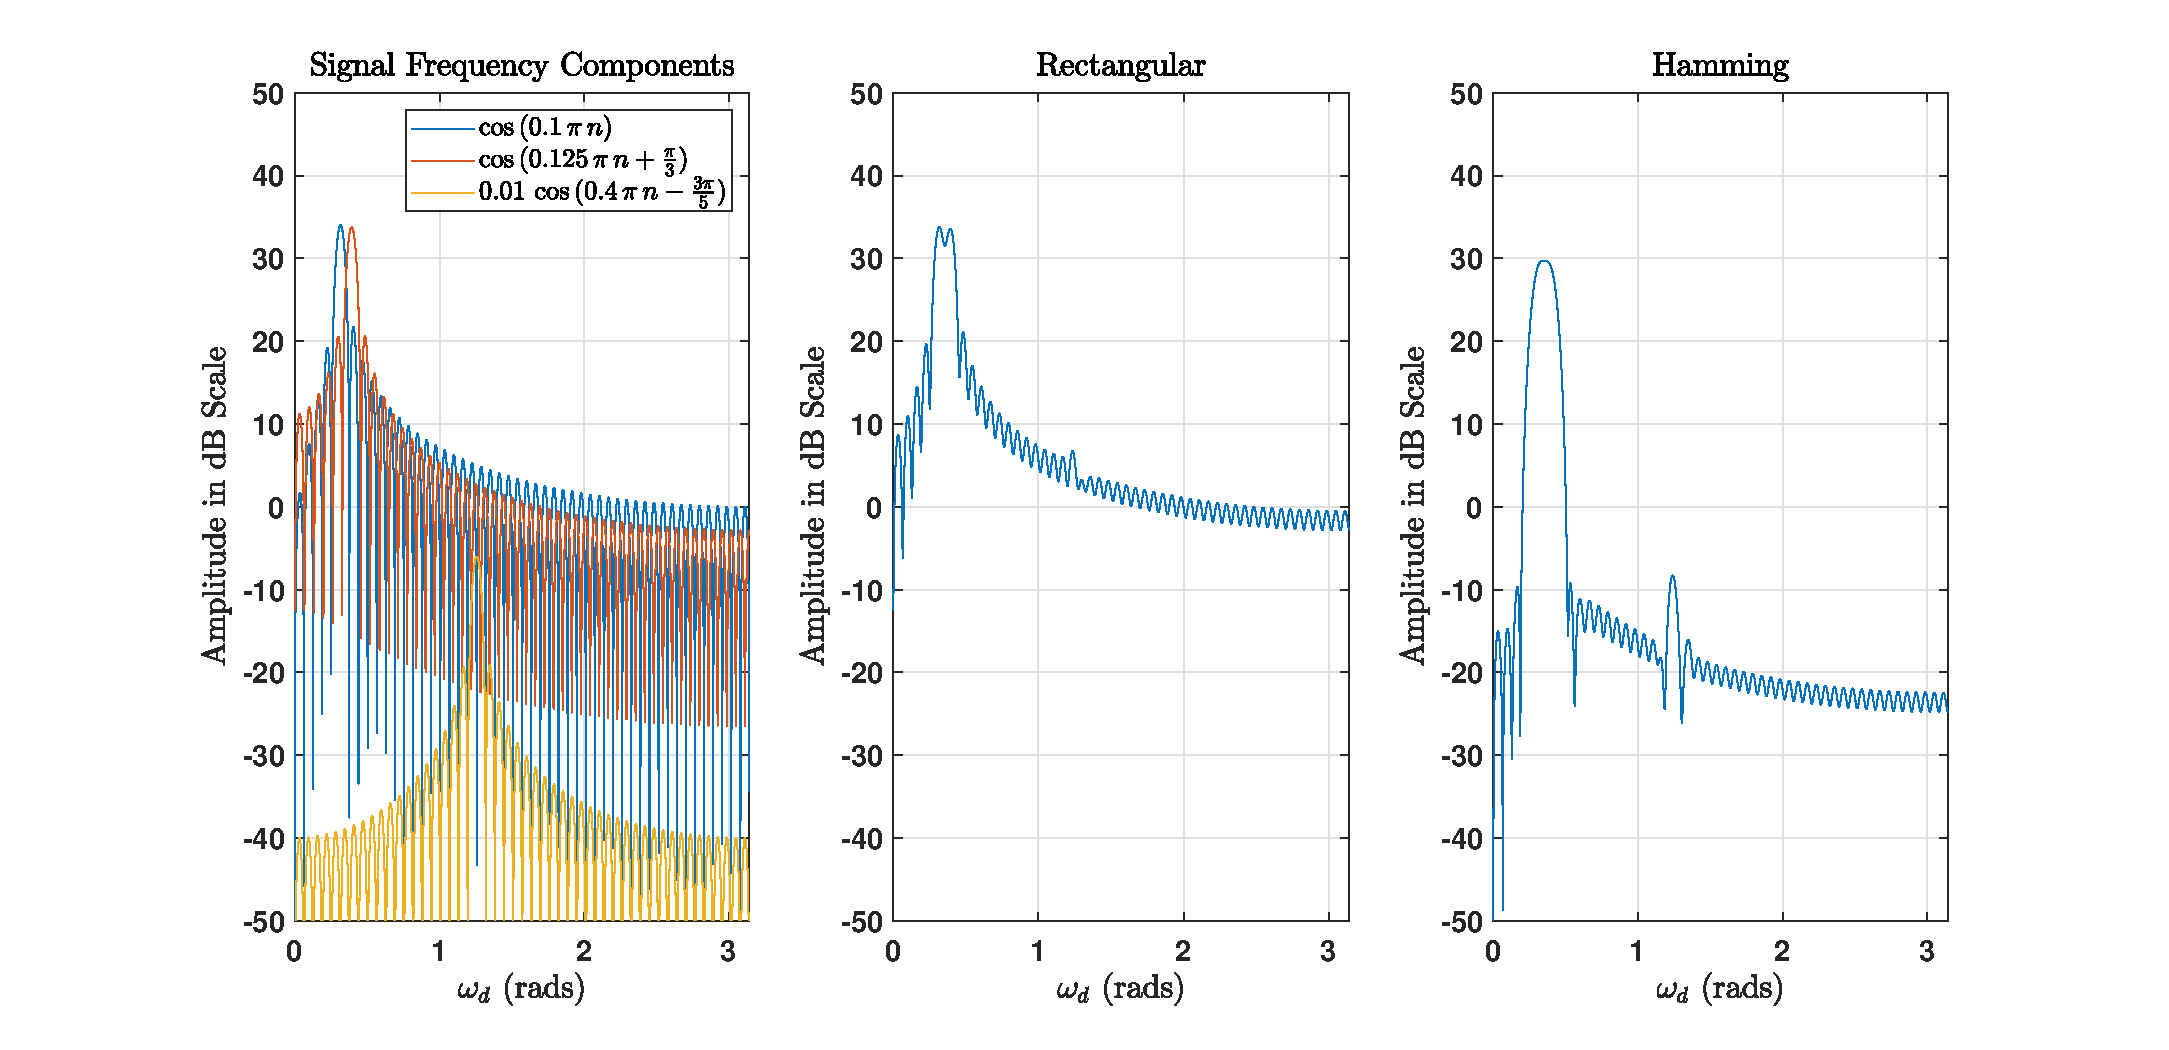
\includegraphics[scale=0.3]{Figures/DFT/sum_of_cos_rect_and_hamm.eps}
\caption{Rectangular and Hamming Window}
\label{fig:Papers:aliasing}
\end{figure}

\newpage
\begin{itemize}

\item In rectangular window:

	\begin{itemize}
	\item the 2 components  can be distinguished
	
	\item However the $\mathrm{3}^\mathrm{rd}$ components having a small amplitude has disappeared in the side lobes

	\begin{itemize}
	\item It barely  we can see it
	
	\item If we have some noisy data, it will completely		 gone
	\end{itemize}		

	\end{itemize}
	
\item In Hamming window:

\begin{itemize}
\item The 2 cos peaks has merged 

\item But the weak components is detected better then the rectangular window
\end{itemize}	
	
\end{itemize}

\newpage

\begin{figure}[h]
\centering
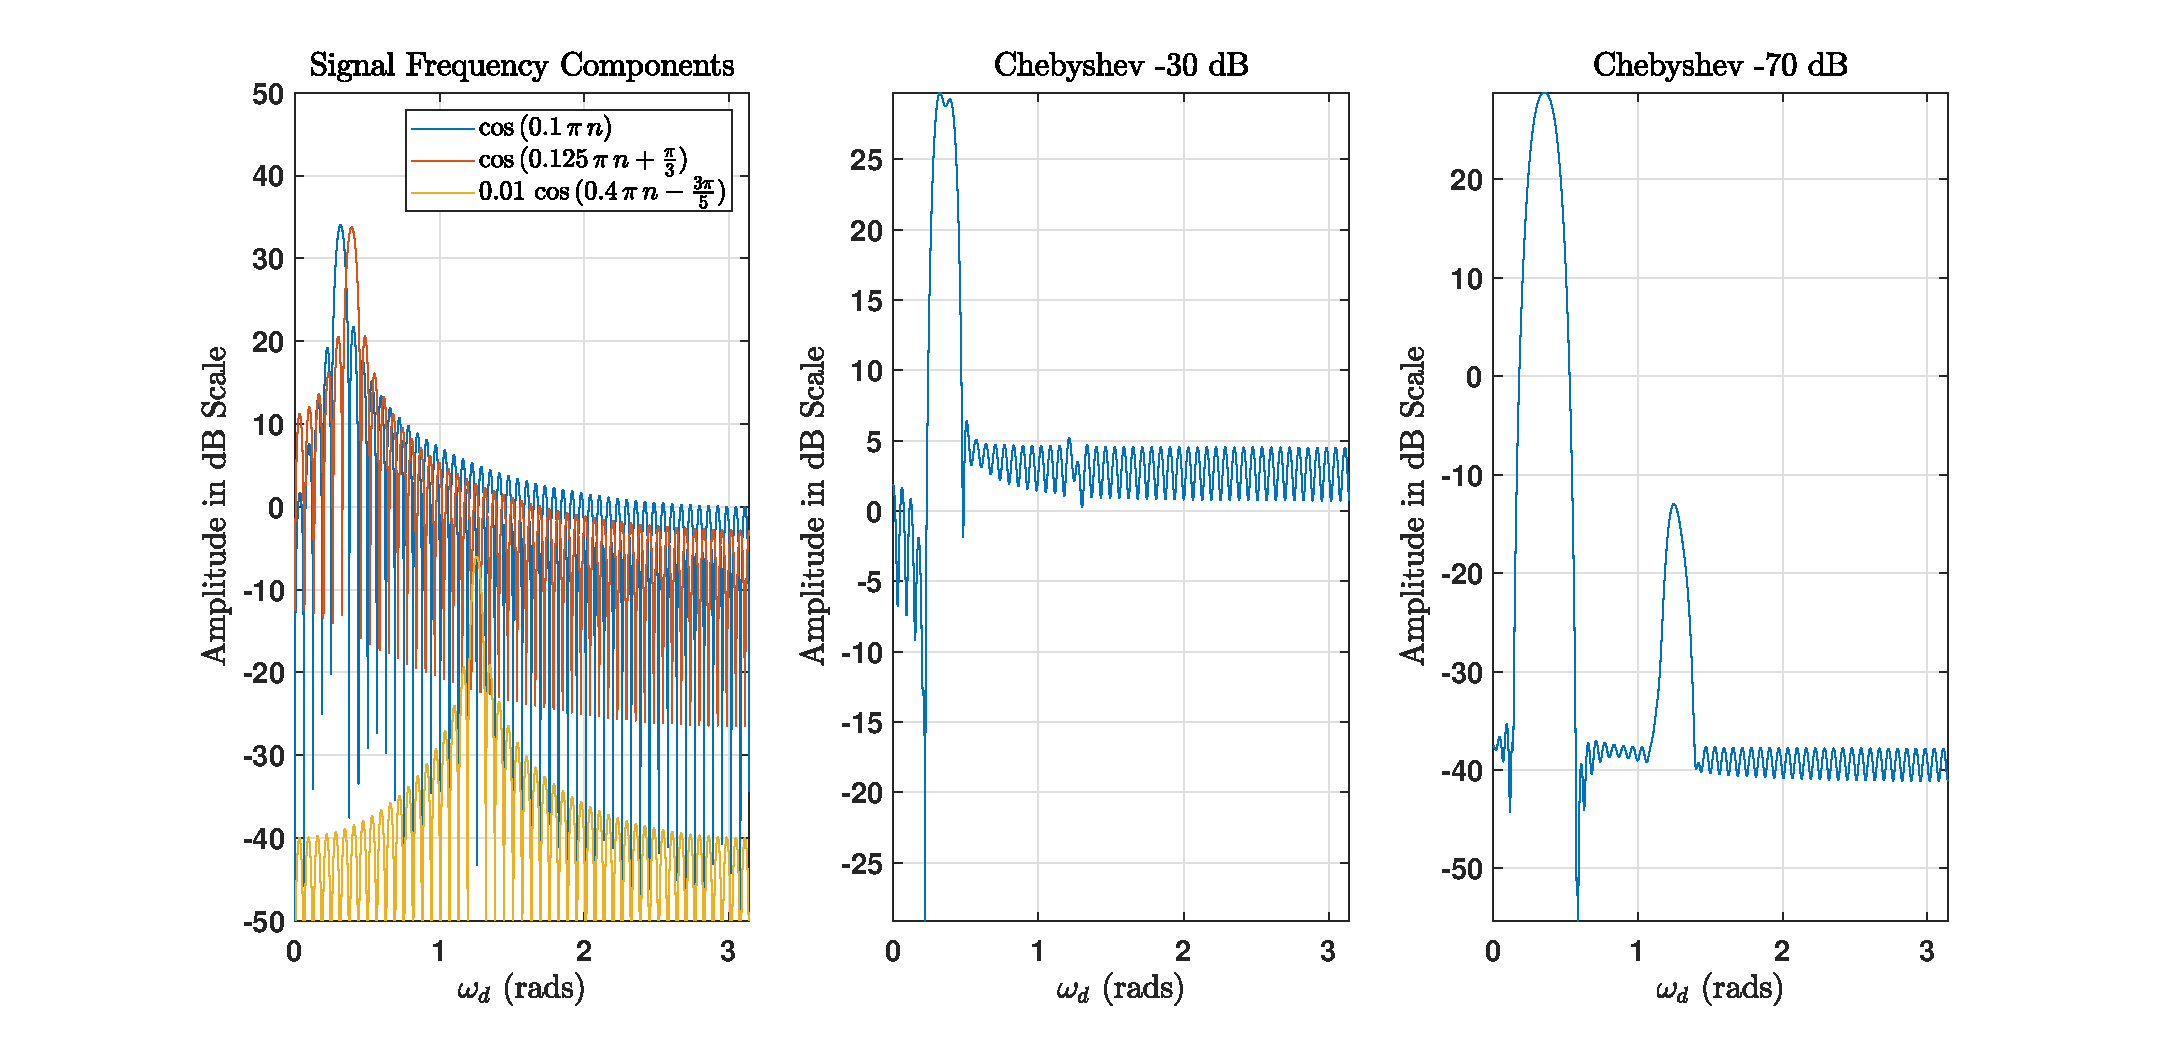
\includegraphics[scale=0.3]{Figures/DFT/sum_of_cos_chebyshev.eps}
\caption{Chebychves Window with -30 dB and -70 dB side lobes attenuation}
\label{fig:DFT:sum_of_cos_chebyshev}
\end{figure}

\newpage

\begin{itemize}

\item In -30 dB case:

	\begin{itemize}
	\item We can (although it is difficult) to see that we have 2 frequency components $\leftrightarrow$ good resolution
	
	\item However the weak component have vanished $\leftrightarrow$ poorer dynamic range
	\end{itemize}

\item In -70 dB case we have opposite results

	\begin{itemize}
	\item Since thee side lobes now are more attenuated, we can detect the weak component
	
	\item Of course in the price of poorer resolution as we can see, the 2 components are gone now
	\end{itemize}

\end{itemize}


\end{frame}


\subsubsection{CTFT Spectrum Using Different Windows}

\begin{frame}[t,allowframebreaks]{Windowed CTFT Spectrum Analysis}

\begin{itemize}

\item We try to see now the effect of windows on CTFT spectrum for a damped cos signals given by:

\begin{equation*}
\begin{array}{rcl}
x(t) \, &=& \, e^{-0.1 \,t} \, \left[\, \text{cos}\left( \, 10 \, t \, \right) \, + \, \text{cos}\left( \, 12 \, t \, \right)  \,\right] \, u(t) \\ \\
X(\omega_c) \, &=& \, \displaystyle\frac{\, 0.1 \, + \, j \, \omega_c}{ \left( \, 0.1 \, + \, j \, \omega_c  \,  \right)^2    \, + \, 10^2} \, + \, \displaystyle\frac{0.1 \,+ \, j \, \omega_c}{ \left( \, 0.1 \, + \, j \, \omega_c  \,  \right)^2    \, + \, 12^2}
\end{array}
\end{equation*}


\begin{figure}[h]
\centering
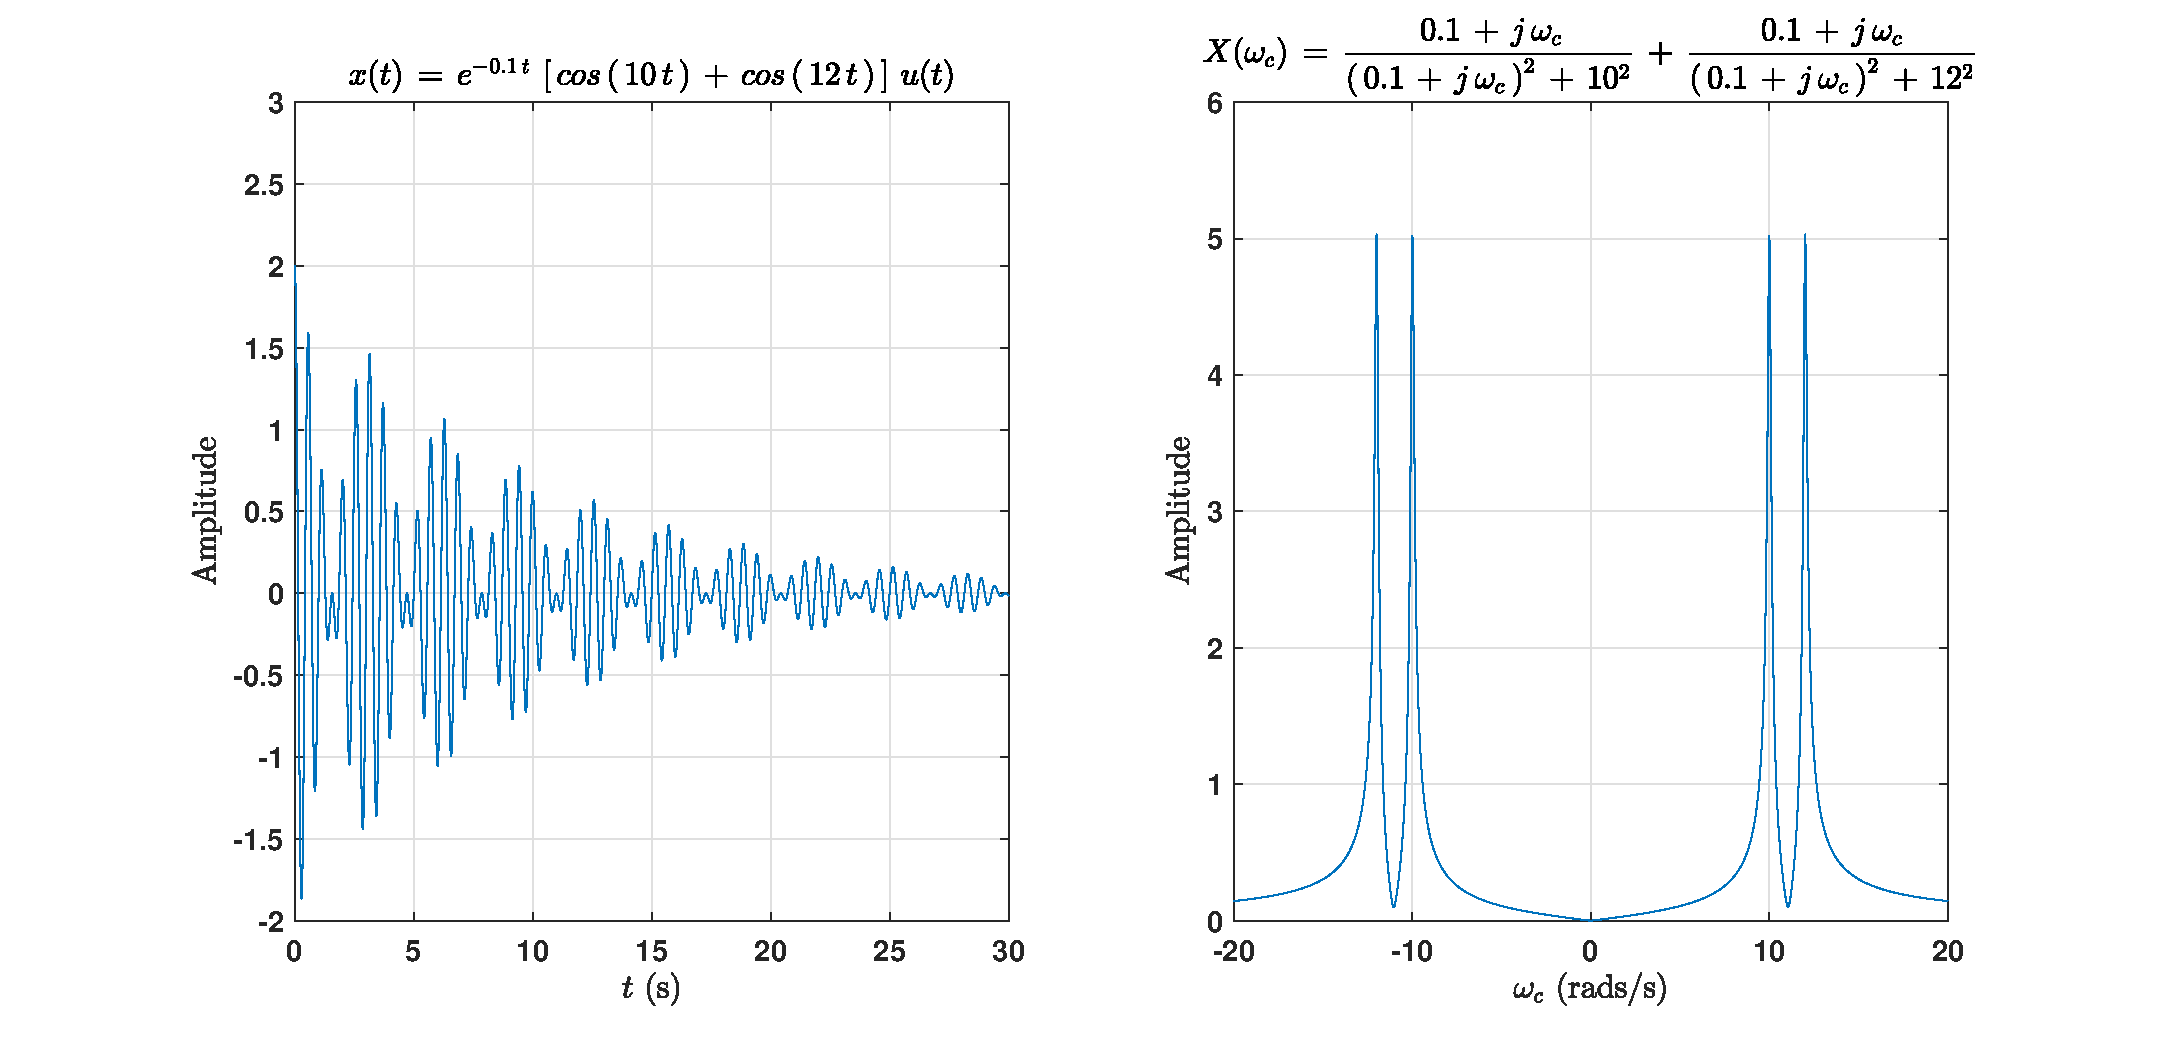
\includegraphics[scale=0.30]{Figures/DFT/damped_cosines_and_spectrum.eps}
\caption{$x(t)$ along with its Amplitude Spectrum}
\label{fig:DFT:damped_cosines_and_spectrum}
\end{figure}

\item $X(\omega_c)$ is not a bandlimited signal, so we need to choose a maximum frequency

	\begin{itemize}
	\item Since we can visualize that after 12 rad/s the spectrum roll off, we choose effective bandwidth of $B \, = \, 300$ rad/s $\rightarrow \, T_s \, = \, 0.01$ s
	\end{itemize}



\item We have 2 damped frequency components at 10 and 12 rad/s. Spectral Separation between these 2 components is $12 \, - \, 10 \,  = \, 2 $ rad/s 

\item Recall that the width of the main lobe need to be smaller than the spectral separation

\newpage
\item We choose to see details at 2 resolution using rectangular window:

	\begin{enumerate}
	\item $\displaystyle\frac{2 \pi}{5} \, \approx \, 1.2566 <<  2$ rad/s
	
		\begin{itemize}
		\item $\displaystyle\frac{4 \pi}{\text{Signal Duration}} \, = \,   \displaystyle\frac{4 \pi}{T_s \, N} \leq \, \displaystyle\frac{2 \pi}{5} \rightarrow \, N \, \geq \, 1000 $ samples
		\end{itemize}
		
	\item We increase resolution times 5: $\displaystyle\frac{2 \pi}{25} \, \approx \, 0.2513$
	
	\begin{itemize}
		\item $\displaystyle\frac{4 \pi}{\text{Signal Duration}} \, = \,   \displaystyle\frac{4 \pi}{T_s \, N} \leq \, \displaystyle\frac{2 \pi}{25} \rightarrow \, N \, \geq \, 5000 $ samples
		\end{itemize}

	\end{enumerate}

\end{itemize}



\end{frame}



\begin{frame}[t,allowframebreaks]{Result and Discussions}


\begin{figure}[h]
\centering
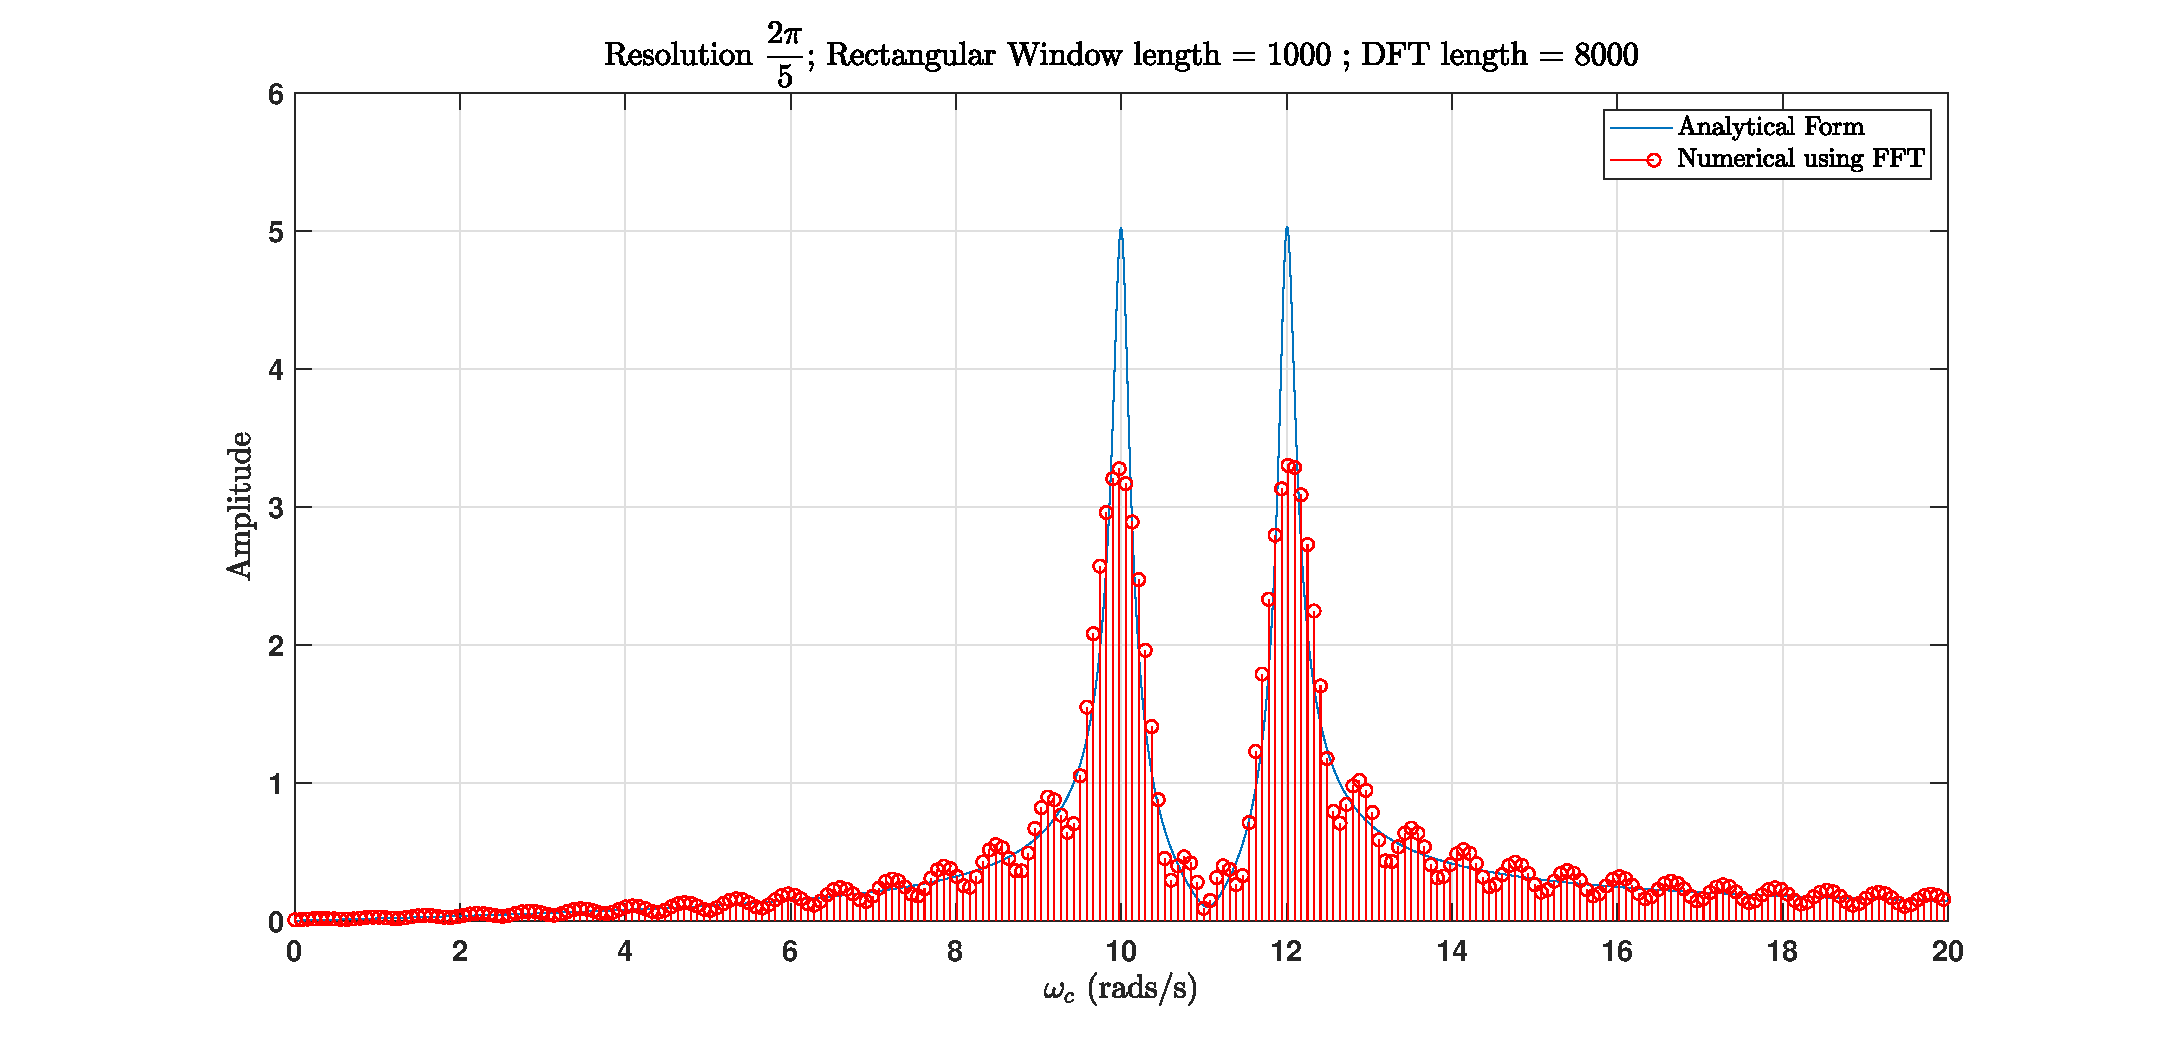
\includegraphics[scale=0.30]{Figures/DFT/spectrum_rect_window_length_1000.eps}
\label{fig:DFT:spectrum_rect_window_length_1000}
\end{figure}

\begin{itemize}

\item DFT Values are distorted

\item Some ripples at the tails

\newpage

\item Increasing resolution 5 times from $\displaystyle\frac{2 \pi}{5} \rightarrow \displaystyle\frac{2 \pi}{25}$ (narrower main lobe)


	\begin{itemize}
	\item Better DFT Values and  No ripples at the tails
	\end{itemize}


\begin{figure}[h]
\centering
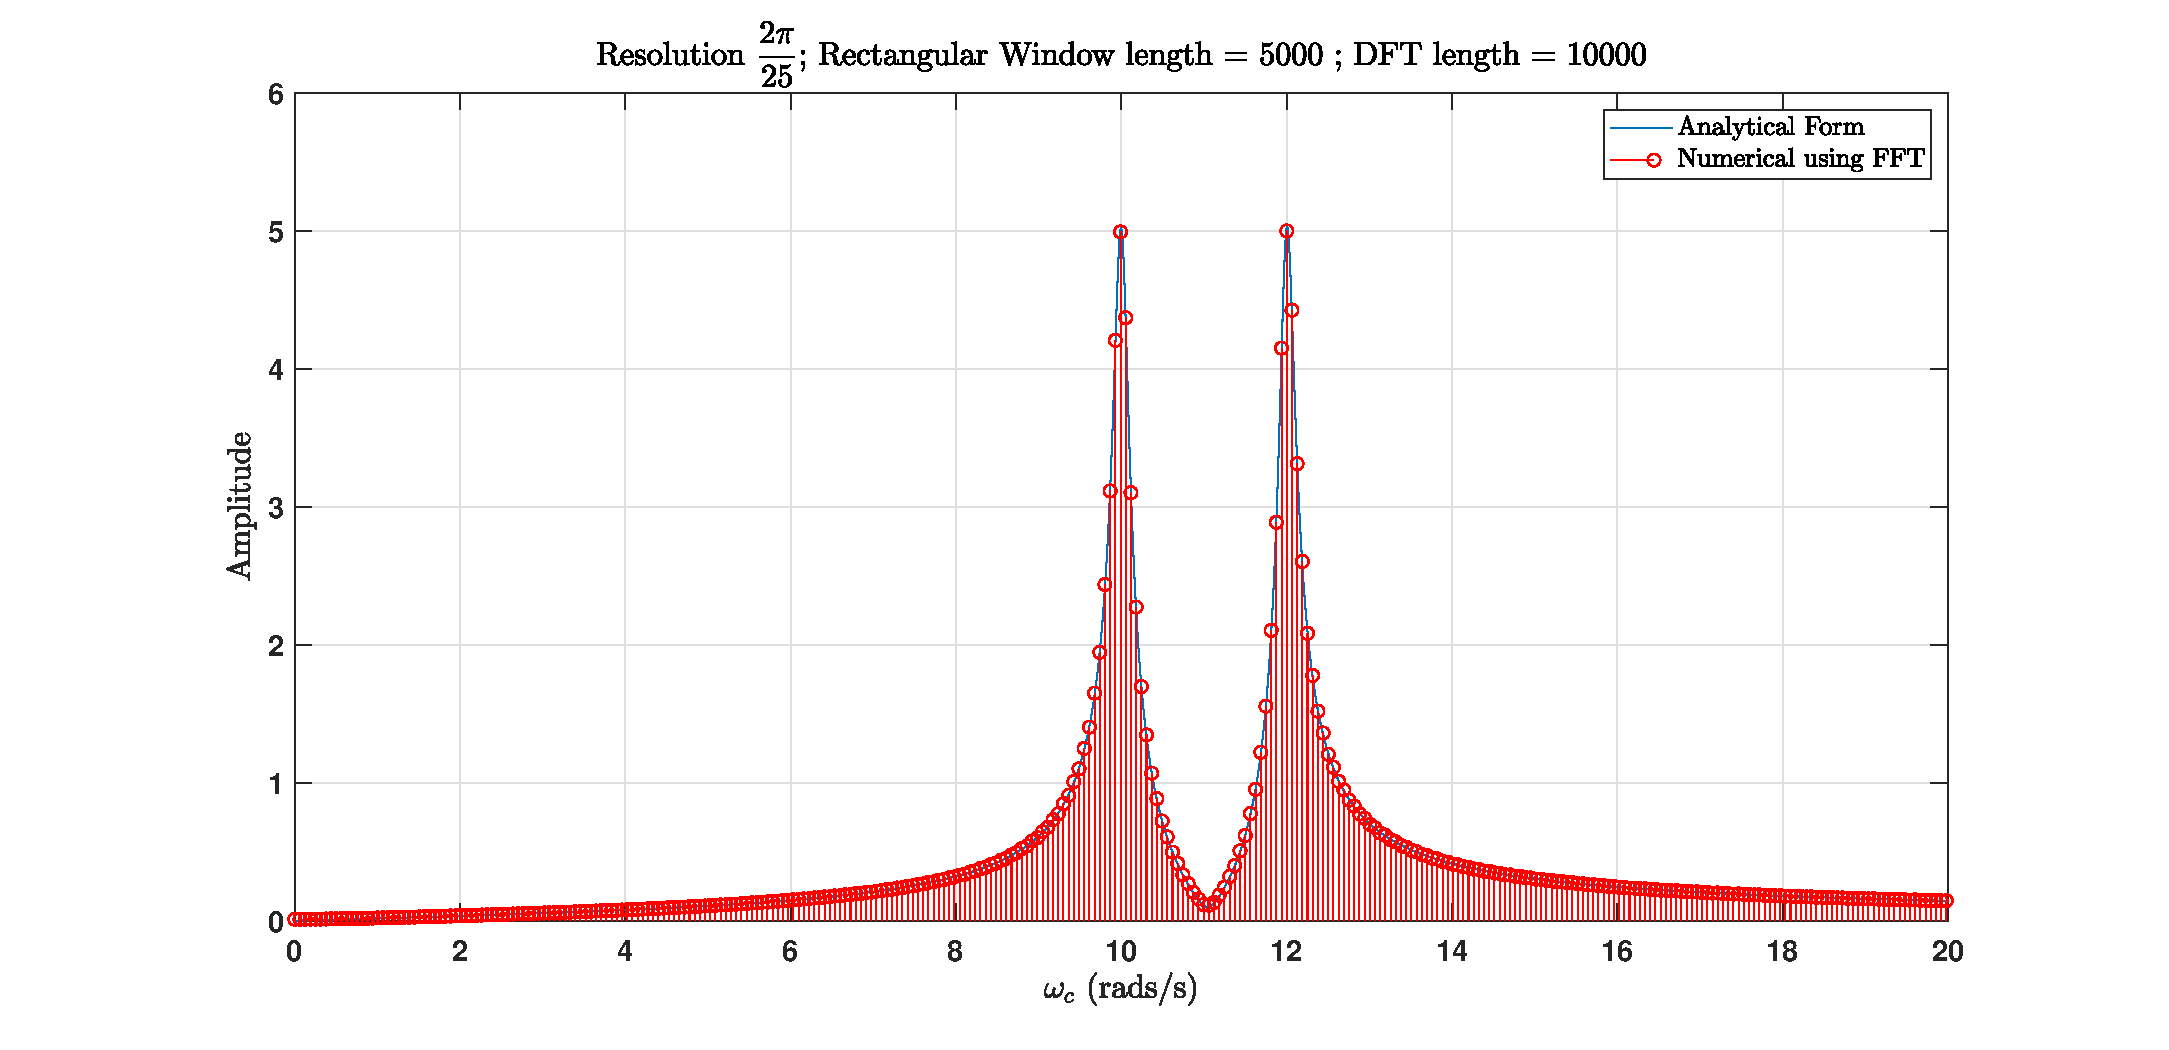
\includegraphics[scale=0.26]{Figures/DFT/spectrum_rect_window_length_5000.eps}
\label{fig:DFT:spectrum_rect_window_length_1000}
\end{figure}



\newpage
\item Trying Different type of Windows: Hamming window for example, with the best observed resolution which is $  \displaystyle\frac{2 \pi}{25}$

\item Hamming Length:

	\begin{itemize}
	\item $\displaystyle\frac{8 \pi}{\text{Signal Duration}} \, = \,   \displaystyle\frac{8 \pi}{T_s \, N} \leq \, \displaystyle\frac{2 \pi}{5} \rightarrow \, N \, \geq \, 10^4 $ samples
	
	\item Rectangular window length was 5000 samples for a resolution  of $  \displaystyle\frac{2 \pi}{25}$
	
	\item Hamming need 2 times more samples then rectangular to observe same level of details
	\end{itemize}


\newpage

\begin{figure}[h]
\centering
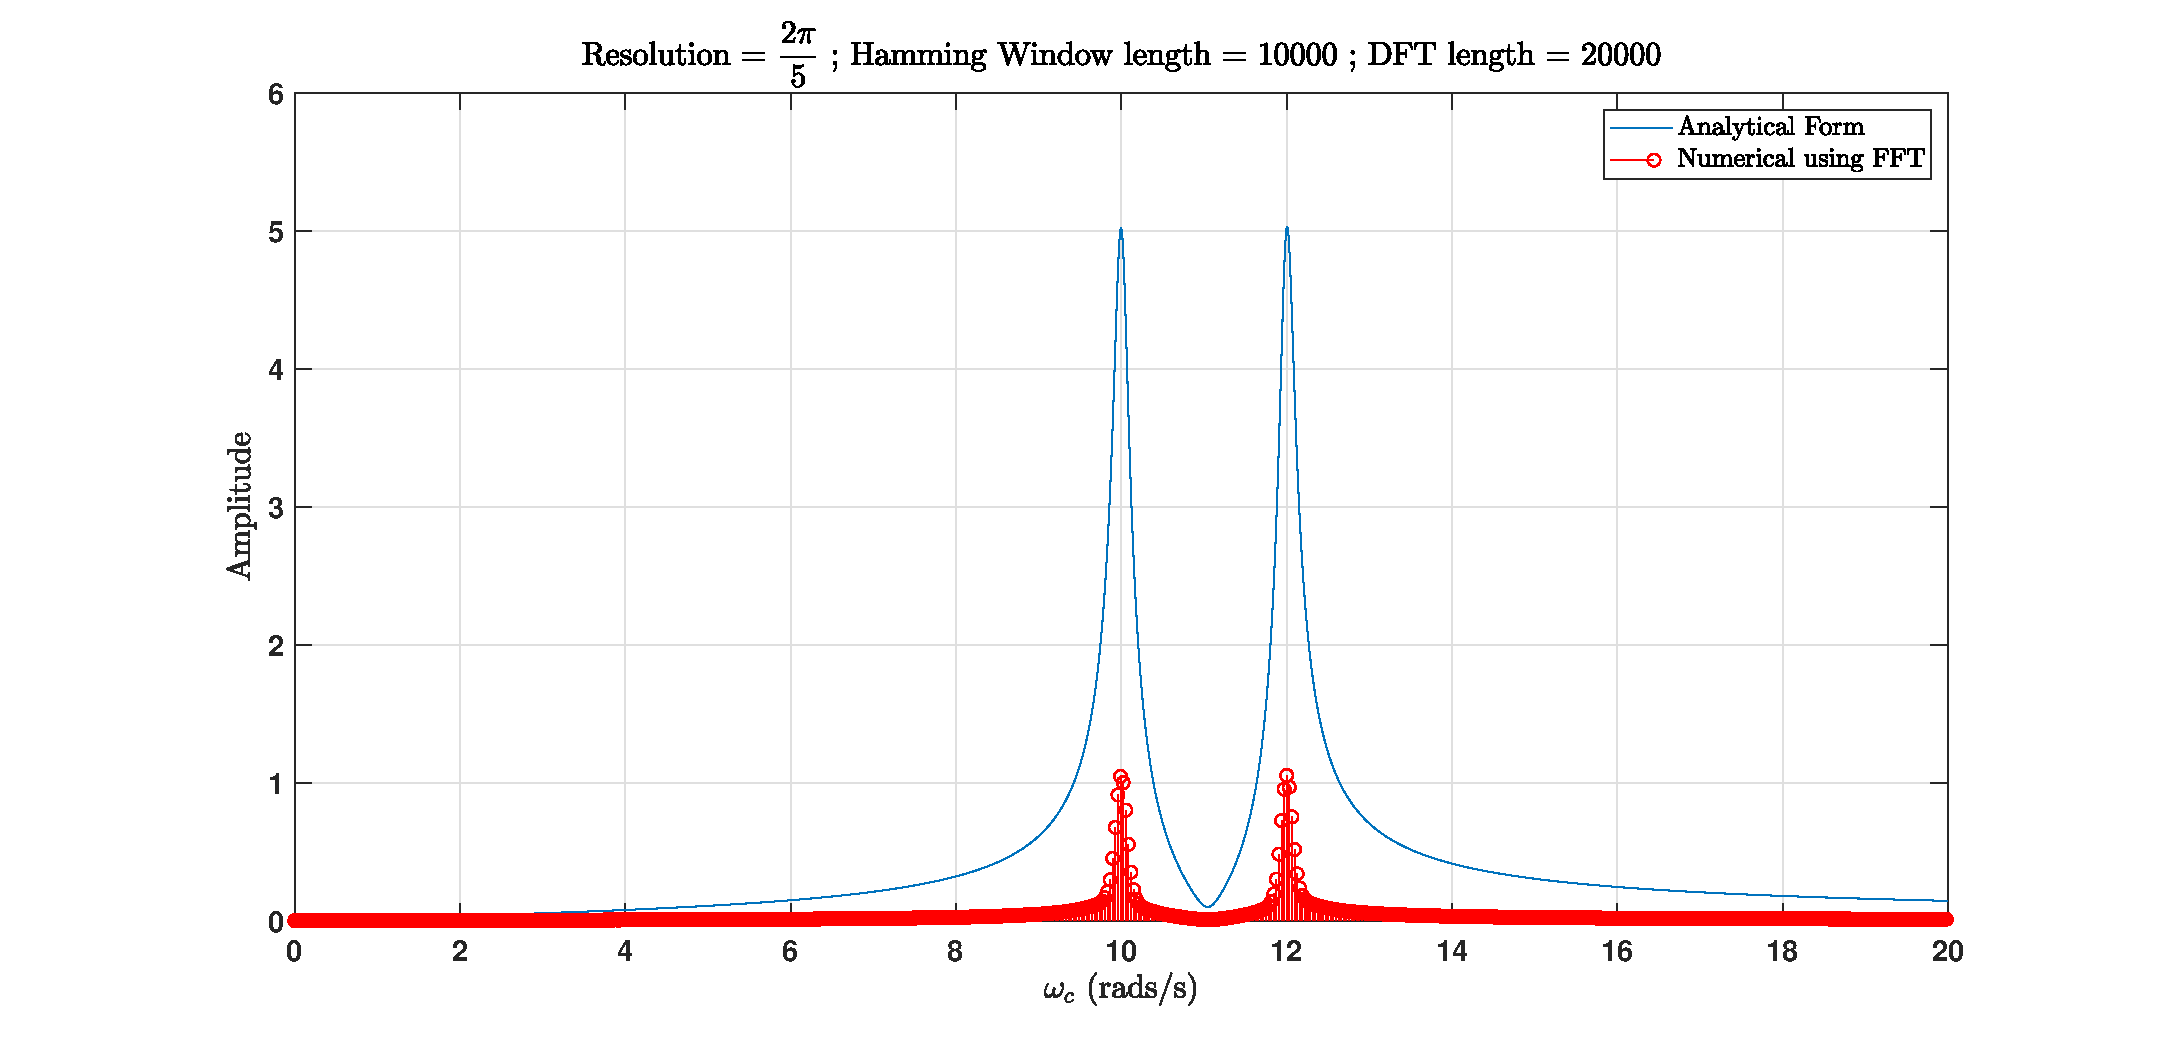
\includegraphics[scale=0.26]{Figures/DFT/spectrum_hamming_window_length_10_pow_4.eps}
\label{fig:DFT:spectrum_hamming_window_length_10_pow_4}
\end{figure}

\item DFT amplitude values are very distorted



\newpage

\item Hamming is attenuating signal energy when we are windowing 

\begin{figure}[h]
\centering
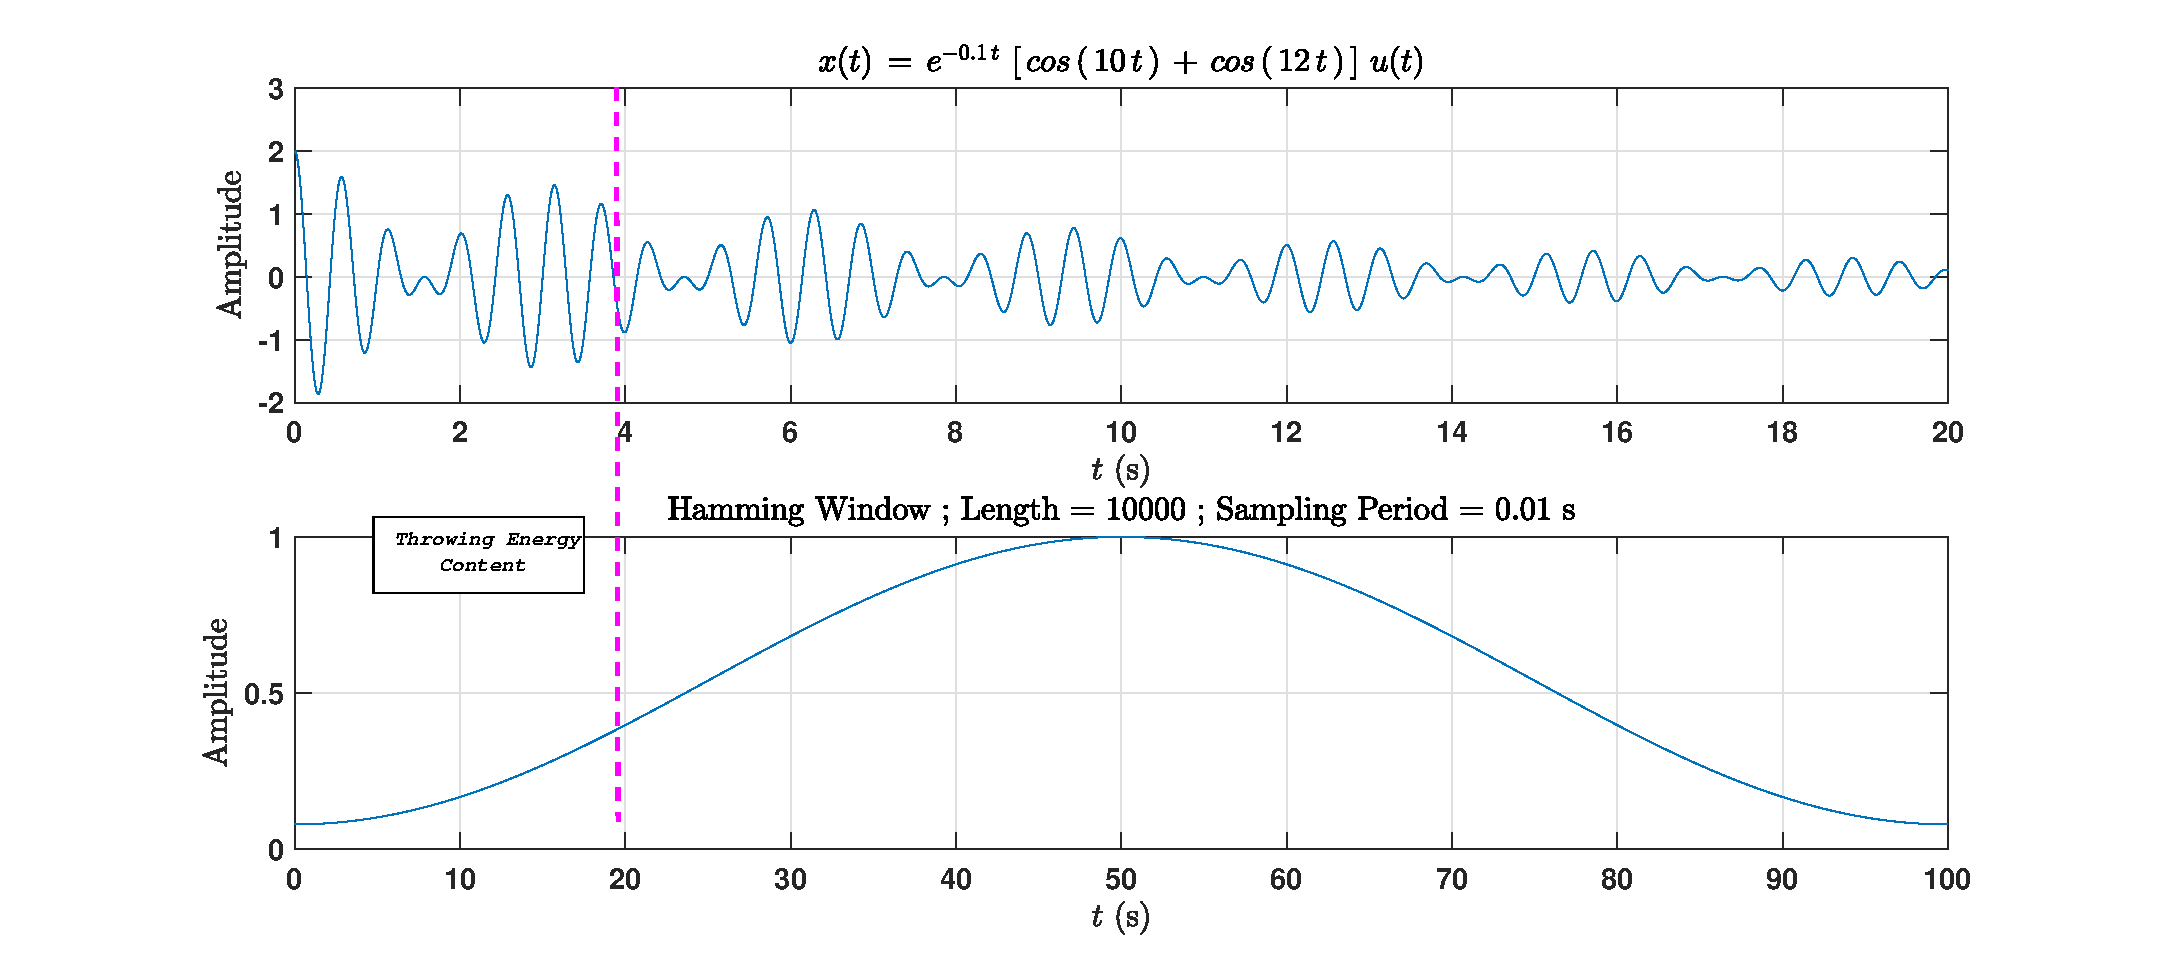
\includegraphics[scale=0.30]{Figures/DFT/hamm_signal_plot_time_domain_2.eps}
\label{fig:DFT:hamm_signal_plot_time_domain_2}
\end{figure}

\end{itemize}


\end{frame}

%**************************************************
%**************************************************
%**************************************************

\section{Time-Frequency Analysis}
\label{Chap:Time-Frequency Analysis}
\begin{frame}[t]{Chapter \autoref{Chap:Time-Frequency Analysis}}
\tableofcontents[sections= \value{section}]
\end{frame}


\subsection{Introduction}
\begin{frame}[t]{Introduction}

\begin{itemize}

\item Time-Frequency analysis is used to analyse non-stationary signals: signals which varies in time

\item Common Tool to this used is called Short-time-Fourier-Transform (STFT)

\end{itemize}

\end{frame}


\subsection{Short Time Fourier Transform}
\begin{frame}[t]{STFT Concepts}

\begin{itemize}

\item Instead of sliding the window on the data, we will do the opposite:

	\begin{itemize}
	\item We fix the window of size $L$
	
	\item We choose an index $n$ which represent the shift in the data $x[m]$: so $n$ represents the start of the segment we are looking on 
	
	\item We make the product between the window and the data
	
	\item Then take the DTFT of this product
	
	
	\item Then we repeat this process for every value of $n \, \rightarrow x[n] \, , \, x[n \, + \, 1] \, , \, \cdots \, x[n \, + \, L - \, 1]$
	\end{itemize}

\item Common Tool to this used is called Short-time-Fourier-Transform (STFT)

\end{itemize}


\end{frame}


\subsection{Temporal and Frequency Resolution Trade-off}
\begin{frame}[t,allowframebreaks]{Temporal and Frequency Resolution Trade-off}

\begin{itemize}

\item From window analysis, we can recall that the higher the window length $\rightarrow$ more frequency details we can capture $\rightarrow$ higher frequency resolution

	\begin{itemize}
	\item However when we do this in STFT, we loose temporal resolution $\leftrightarrow$ we can't observe details in time domain in the time-frequency plane
	\end{itemize}

\item If we decrease the window size, the resolution in frequency content decrease

	\begin{itemize}
	\item For a window size $L \, = \, 128$ Along the vertical axis (frequency axis), we can't capture that we have 2 frequencies at 250 Hz and 300 Hz
	
	\item However for this same window size, we get a better temporal resolution $\leftrightarrow$ we can indentify the moment of transition from 300 Hz $\rightarrow$ 250 Hz
	\end{itemize}


\end{itemize}


\end{frame}

%**************************************************
%**************************************************
%**************************************************

\section{$Z$ Transform}
\label{Chap:z_transform}
\begin{frame}[t,allowframebreaks]{Chapter \autoref{Chap:z_transform}}
\tableofcontents[sections= \value{section}]
\end{frame}


\subsection{Complex Exponential Signal}
\begin{frame}[t,allowframebreaks]{Some Preliminary}

\begin{itemize}

\item Before we dive in the definition of $Z$-transform, let's see what is this number called $z$

	\begin{itemize}
	\item This will give us some intuition since we use this number in the definition oft the $Z$-transform
	\end{itemize}

\item $z$ is just a \textcolor{red}{complex number} 

\item We prefer to write in polar form as $z \, = \, r \, e^{j \, \Omega}$

\item If we form a signal called $x[k] \, = \, z^{k}$, it will be a \textcolor{red}{discrete time complex signal}, where using Euler identity we have:

\begin{equation*}
x[k] \, = \, z^{k} \, = \, r^k \, \left[\, \text{cos}(\Omega \, k) \, + \, \text{sin}(\Omega \, k)  \,\right]
\end{equation*}

	\begin{itemize}
	\item $r$ controls the damping of this signal
	
	\item and $\Omega$ controls the frequency
	\end{itemize}

\newpage
\item An example is shown in figure \autoref{fig:z_transform:exp_signal} for $r \, < \, 1$

\begin{figure}[h]
\centering
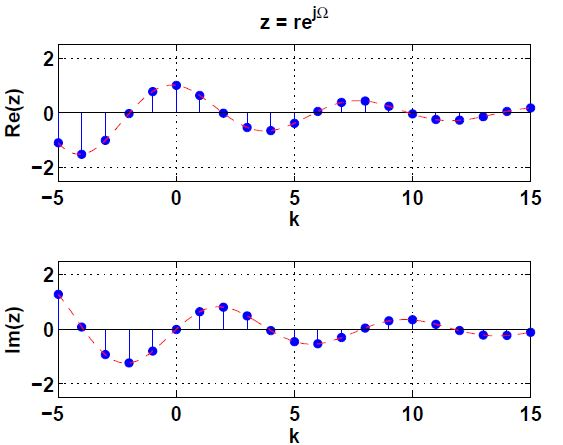
\includegraphics[scale=0.3]{Figures/z_transform/exp_signal}
\caption{Complex Exponential Discrete Signal}
\label{fig:z_transform:exp_signal}
\end{figure}


\end{itemize}

\end{frame}

\subsection{Eigenfunction Property} 
\begin{frame}[t,allowframebreaks]{Eigenfunction Property}

\begin{itemize}

\item In this part we will now why we are interested in power signal $z^k$ 

\item We will apply $z^k$ as an input to discrete linear-time invariant system

\item Computation:


$\begin{array}{rcl}
y[k] \, &=& \, h[k] \, * x[k] \\ \\
		&=& \, \displaystyle\sum_{m \, = \, - \infty}^{+ \infty} h[m] \, \times \, x[k \, - \, m] \\
		&=& \, \displaystyle\sum_{m \, = \, - \infty}^{+ \infty} h[m] \, \times \, z^{k \, - \, m} \\ \\
		&=& \, z^k \, \times \, \left(\, \displaystyle\sum_{m \, = \, - \infty}^{+ \infty} h[m] \, \times \, z^{- \, m} \, \right)\\
		&& \, \text{We pull out } z^k \text{ since the summation is a function of } m
\end{array}$

\item For a exponential input signal $z^k$, the \textcolor{red}{response} $y$ is a \textcolor{red}{scaled version} of the input signal $z^k$

\item The signal  $z^k \, = \, (r \, e^{j \, \Omega})^k$ is called \textcolor{red}{eigenfunction} because an eigenfunction applied to a system, \textcolor{red}{give output = to the input but with a scaling factor}

\end{itemize}


\end{frame}

\subsection{Transfer function}
\begin{frame}[t,allowframebreaks]{Transfer function}

\begin{itemize}

\item In the computations of the response of the complex exponential signal, the scaled version is a special quantity called \textcolor{red}{transfer function} $H(z)$ defined as:

\begin{equation}
H(z) \, = \, \displaystyle\sum_{k \, = \, - \infty}^{+ \infty} h[k] \, \times \, z^k
\end{equation}

where $h[k]$ is the impulse response of the discrete time LTI system.

\end{itemize}

\end{frame}

\subsection{Summary}
\begin{frame}[t,allowframebreaks]{Summary Eigenfunction Property}

\begin{itemize}

\item For a complex exponential signal $z^k \, = \, (r \, e^{j \, \Omega})^k$ applied as input, we get the following response

\begin{equation}
\begin{array}{rcl}
y[k] \, &=& \, z^k \, \times \, \displaystyle\sum_{m \, = \, - \infty}^{+ \infty} h[m] \, \times \, z^m \\ \\
&=& \, H(z) \, \times \, z^k  
\end{array}
\end{equation}

	\begin{itemize}
	\item $z^k$ \textcolor{red}{eigenfunction} of the system with associated eigenvalue $H(z)$ 
	\end{itemize}


\item As any complex number, $H(z) \, = \, |H(z)| \, e^{j \, \phi(z)}$, so we can further develop the response $y[k]$ as:

\begin{equation}
\begin{array}{rcl}
y[k] \, &=& \, z^k \, \times \, \displaystyle\sum_{m \, = \, - \infty}^{+ \infty} h[m] \, \times \, z^{-m} \\ \\
&=& \, H(z) \, \times \, z^k \\ \\
&=& |H(z)| \, e^{j \, \phi(z)}   \times \, z^k 
\end{array}
\end{equation}

	\begin{itemize}
	\item Interpretation: the system $H(z)$ \textcolor{red}{change only} the \textcolor{red}{amplitude} and the \textcolor{red}{phase} of the \textcolor{red}{input signal} $z^k$
	
	\item But it \textcolor{red}{won't change its frequency} $\Omega$
	\end{itemize}

\end{itemize}


\end{frame}


\subsection{Definitions}
\begin{frame}[t,allowframebreaks]{$Z$-Transform Definitions}

\begin{definition}

The \textcolor{red}{bilateral $z$-transform} of a discrete time signal $x[k]$ is:

\begin{equation}
X(z) \, = \, \displaystyle\sum_{k \, = \, - \infty}^{+ \infty} x[k] \, \times \, z^{-k} 
\end{equation}

\end{definition}

\begin{definition}

The \textcolor{red}{inverse bilateral z-transform} of a $X[z]$ is:

\begin{equation}
x[k] \, = \, \displaystyle\frac{1}{2 \, \pi \, j} \displaystyle\oint X(z) \, z^{k \, - \, 1} \, dz
\end{equation}

\end{definition}

\newpage
\begin{itemize}

\item In most of the times we are going to use the bilateral definition of the z-transform

	\begin{itemize}
	\item But also we will use the \textcolor{red}{unilateral} definition for \textcolor{red}{causal signals}
	
	\item Make life easier when dealing with region of convergence issues
	\end{itemize}

\item We won't apply complex contour integral to compute the inverse z-transform

	\begin{itemize}
	\item Instead, we will deal with simpler methods 
	\end{itemize}

\end{itemize}

\end{frame}

\subsection{Convergence}
\begin{frame}[t,allowframebreaks]{Convergence}

\begin{itemize}

\item The $z$-transform definition involves infinite summation

	\begin{itemize}
	\item Whenever we do an infinite sum, we ask the question  when does this sum converge ?
	\end{itemize}

\item Back to the definition of $z$-transform, the sum will converge if we have if the product $x[k] \, \times \, z^{-k}$ is \textcolor{red}{absolute summable}

\item Let's decompose $x[k] \, \times \, z^{-k}$:

	\begin{itemize}
	\item Recall that $z \, = \, r \, e^{j \, \Omega}$
	
	\item $\lvert \,x[k] \,z^{-k}  \,\rvert \, = \, \lvert \,x[k] \,r^{-k} \, e^{-k \, j \, \Omega}  \,\rvert \, = \lvert \,x[k] \,r^{-k} \,\rvert$
	\end{itemize}

\item So $z$-transform when $\displaystyle\sum_{k \, = \, - \infty}^{+ \infty} \lvert \,x[k] \,r^{-k} \,\rvert \, < \, \infty$

	\begin{itemize}
	\item Values of $r$ for which we have convergence is called \textcolor{red}{region of convergence}
	\end{itemize}

\end{itemize}


\end{frame}

\begin{frame}[t,allowframebreaks]{Convergence Example: DTFT and $Z$-transform}

\begin{itemize}

\item We take the following discrete time signal

\begin{figure}[h]
\centering
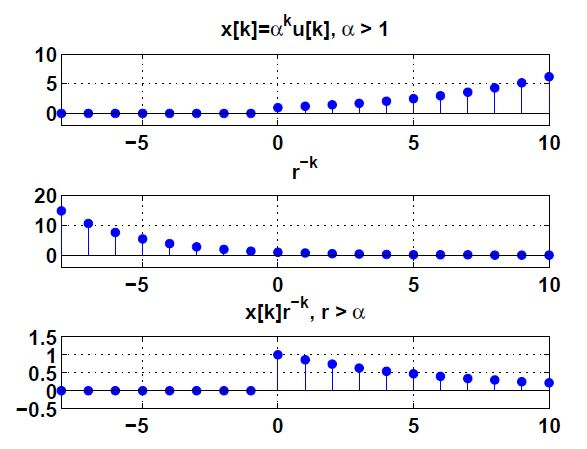
\includegraphics[scale=0.3]{Figures/z_transform/convergence_example}
\caption{DTFT of $x[k]$ doesn't exist, but z-transform exist}
\label{fig:z_transform:convergence_example}
\end{figure}

\newpage
\item $x[k]$ is increasing

	\begin{itemize}
	\item So the DTFT computation can't be done since the signal won't converge
	\end{itemize}

\item However, in Z-transform, we don't only look a the signal $x[k]$, but also with the free variable $r$

	\begin{itemize}
	\item Notice for a value $r \, > \, \alpha$, the product $x[k] \, r^{-k}$ decrease in discrete time
	\end{itemize}

\end{itemize}

\end{frame}

\begin{frame}[t,allowframebreaks]{The $Z$-Plane and DTFT}

\begin{itemize}

\item We have talked about the definition of the $z$-transform, and its convergence

\item One final point before application is the $Z$-plane

\item The $z$-plane is just a complex plane where we have the real and imaginary part of $z$ for various value of $r$ and $\Omega$


\newpage

\item A plot is shown in figure \autoref{fig:z_transform:z_plane}.

\begin{figure}[h]
\centering
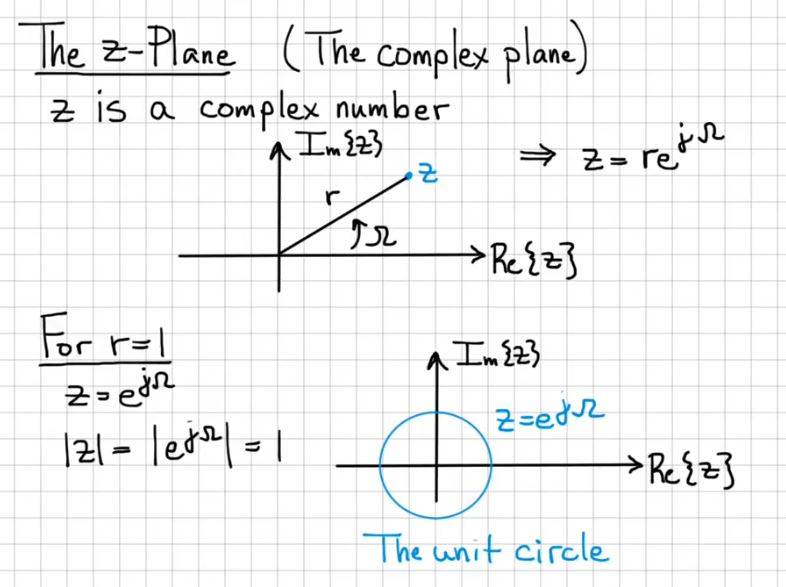
\includegraphics[scale=0.3]{Figures/z_transform/z_plane}
\caption{Z-plane Plot}
\label{fig:z_transform:z_plane}
\end{figure}

\end{itemize}

\end{frame}

\begin{frame}[t,allowframebreaks]{DTFT and Z-transform Relation}

\begin{itemize}

\item One important thing we can notice that is if set $r \, = \, 1$ and apply the definition of the $Z$-transform we get:

$\begin{array}{rcl}
X(z) \, = \, \displaystyle\sum_{k \, = \, - \infty}^{+ \infty} x[k] \, \times \, z^{-k} \, = \, \displaystyle\sum_{k \, = \, - \infty}^{+ \infty} x[k] \, \times \, r^{-k} \, e^{-j \, k \, \Omega} \, = \, \\ \displaystyle\sum_{k \, = \, - \infty}^{+ \infty} x[k] \, \times \, 1 \, \times  \, e^{-j \, k \, \Omega} \, = \,
\displaystyle\sum_{k \, = \, - \infty}^{+ \infty} x[k] \, \times \, e^{-j \, k \, \Omega}  
\end{array}$

\item So for $r \, = \, 1$, we can extract the DTFT from the $Z$-transform

	\begin{itemize}
	\item In other words, from the points on the unit circle in the $z$-plane
	\end{itemize}

\end{itemize}


\end{frame}


\subsection{Examples}

\begin{frame}[t,allowframebreaks]{Example 1: Finite Duration Discrete Time Signal}

\begin{itemize}

\item Given and Solution

\begin{figure}[h]
\centering
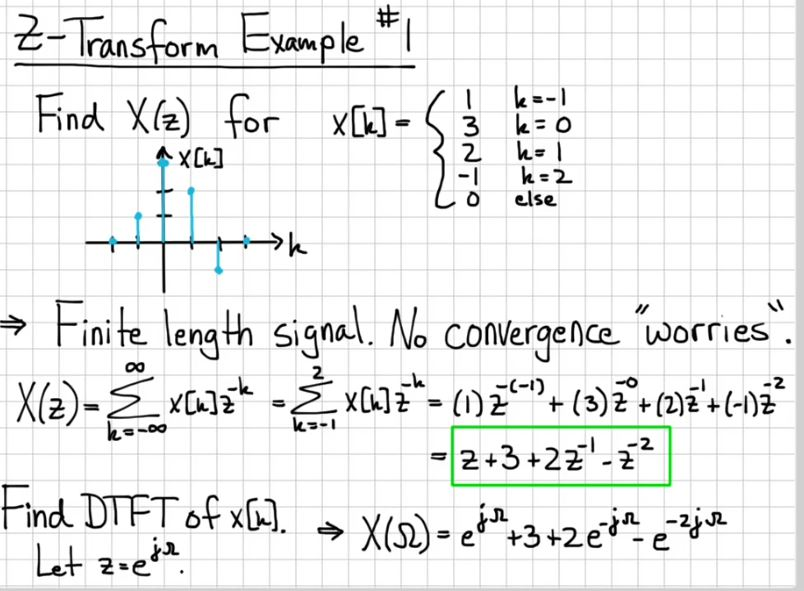
\includegraphics[scale=0.3]{Figures/z_transform/example_finite_duration}
\label{fig:z_transform:example_finite_duration}
\end{figure}

\item Since the signal is finite duration $\leftrightarrow$ no worries about convergence issues

\item We can evaluate DTFT of $x[k]$ by evaluating the z-transform at $r \, = \, 1$

\item Since the \textcolor{red}{region of convergence contains the unit circle}, we can use $z \, = \, e^{j \, \omega_d}$

\item The only points which are outside the region of convergence for a z-polynomial are 0 and $\pm \infty$

\end{itemize}


\end{frame}



\subsubsection{Finite Duration Causal Discrete Time Signal with multiples poles and zeros}
\begin{frame}[t,allowframebreaks]{Example 2: Infinite Duration Causal Discrete Time Signal}

\begin{figure}[h]
\centering
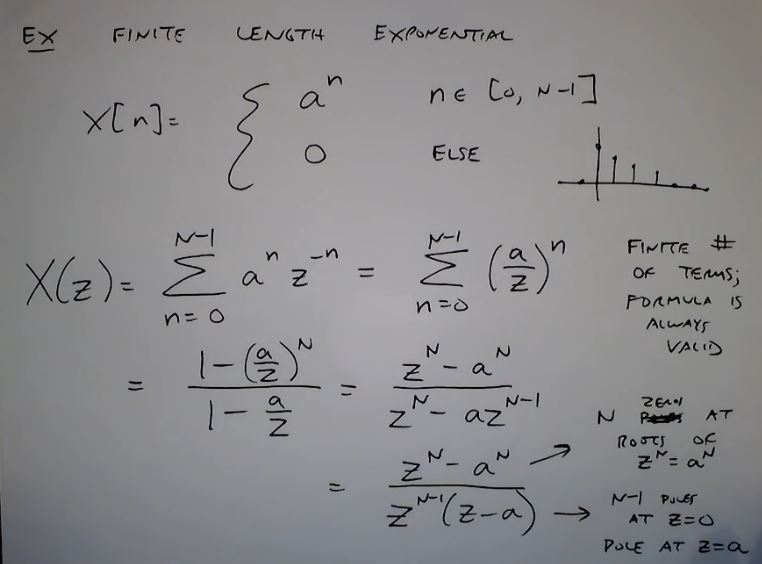
\includegraphics[scale=0.3]{Figures/z_transform/example_finite_duration_causal_many_poles_1}
\end{figure}

\newpage
\begin{figure}[h]
\centering
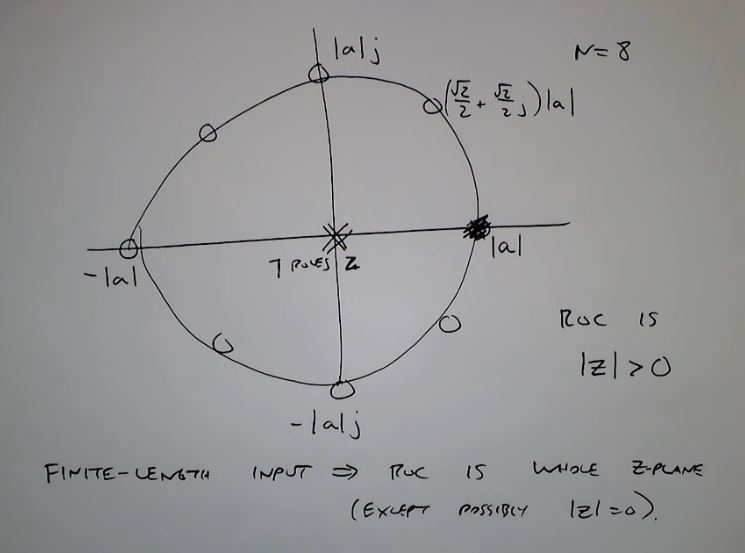
\includegraphics[scale=0.3]{Figures/z_transform/example_finite_duration_causal_many_poles_2}
\end{figure}


\end{frame}



\subsubsection{Infinite Duration Causal Discrete Time Signal}
\begin{frame}[t,allowframebreaks]{Example 2: Infinite Duration Causal Discrete Time Signal}

\begin{itemize}

\item Given and Solution

\begin{figure}[h]
\centering
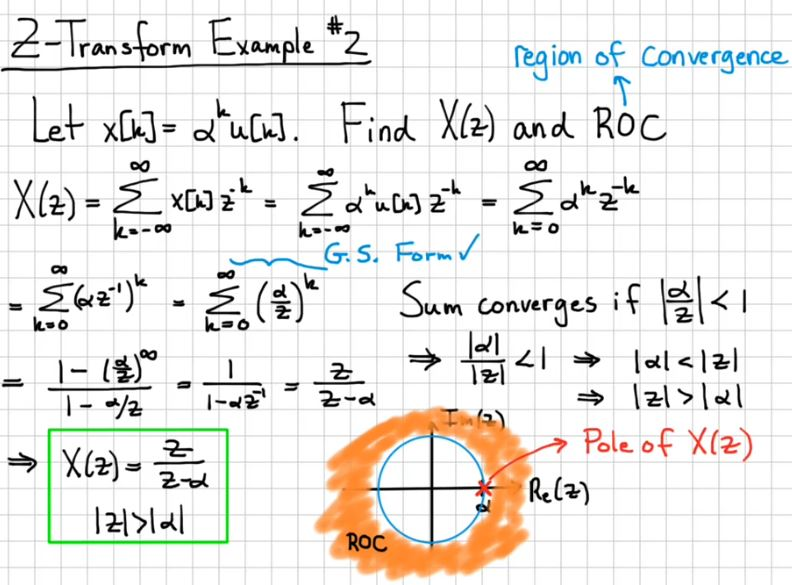
\includegraphics[scale=0.3]{Figures/z_transform/example_infinite_duration_causal_signal}
\label{fig:z_transform:example_infinite_duration_causal_signal}
\end{figure}

\newpage
\item We use the geometric series formula to evaluate the sum

\item Before directly using the geometric series formula, we need to determine the convergence since we have $\left( \, \displaystyle\frac{\alpha}{z} \, \right)^k$

\item The points outside the circle of radius $\alpha$ is the region of convergence

	\begin{itemize}
	\item For a points at $\alpha$, $X(z) \rightarrow \, \infty$
	\end{itemize}

\end{itemize}

\end{frame}


\subsubsection{Infinite Duration Anti-Causal Discrete Time Signal}
\begin{frame}[t,allowframebreaks]{Example 3: Infinite Duration Anti-Causal Discrete Time Signal}

\begin{itemize}

\item Given and Solution

\begin{figure}[h]
\centering
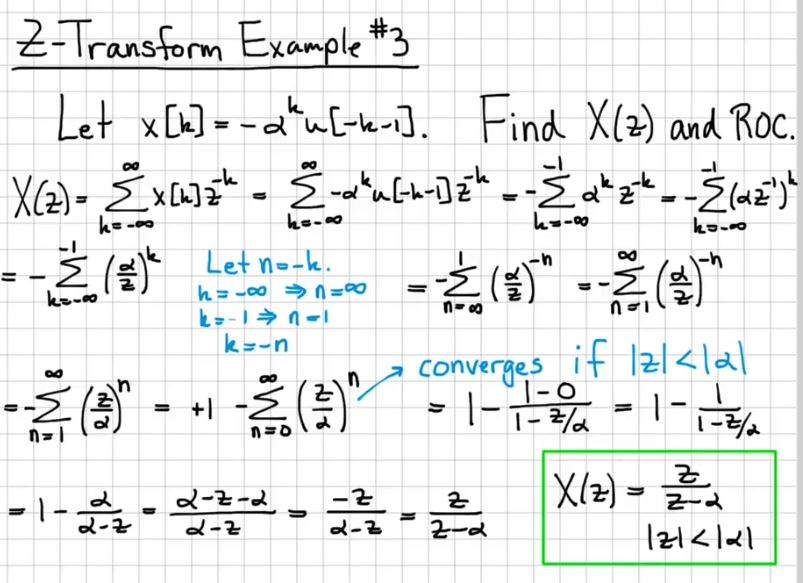
\includegraphics[scale=0.3]{Figures/z_transform/example_infinite_duration_anticausal_signal}
\label{fig:z_transform:example_infinite_duration_anticausal_signal}
\end{figure}

\item In the computation step where we have $ - \, \displaystyle\sum_{n \, = \, 1}^{\infty} \left( \, \displaystyle\frac{z}{\alpha} \, \right)^n \, = \, +1 \, - \,  \displaystyle\sum_{n \, = \, 0}^{\infty} \left( \, \displaystyle\frac{z}{\alpha} \, \right)^n $:

	\begin{itemize}
	\item We have change the summation limits from $n \, = \, 1 \rightarrow \, n \, = \, 0$, so we have add a -1 term (since we have $-$ outside), so we need to add +1 to compensate the result
	\end{itemize}

\newpage

\begin{figure}[h]
\centering
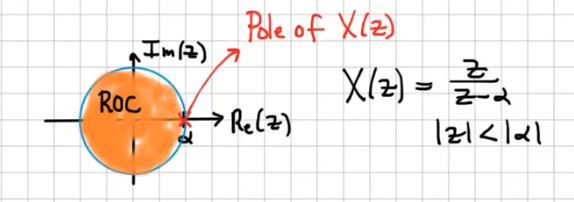
\includegraphics[scale=0.6]{Figures/z_transform/example_infinite_duration_anticausal_signal_roc}
\label{fig:z_transform:example_infinite_duration_anticausal_signal_roc}
\end{figure}

\end{itemize}

\end{frame}


\subsubsection{2 Causal Signals}
\begin{frame}[t]{2 Causal Signals}

\begin{itemize}
    \item If we have 2 signals which adds up, then the resulting ROC is the intersection of the individual ROC of each signal
    
\begin{figure}[h]
\centering
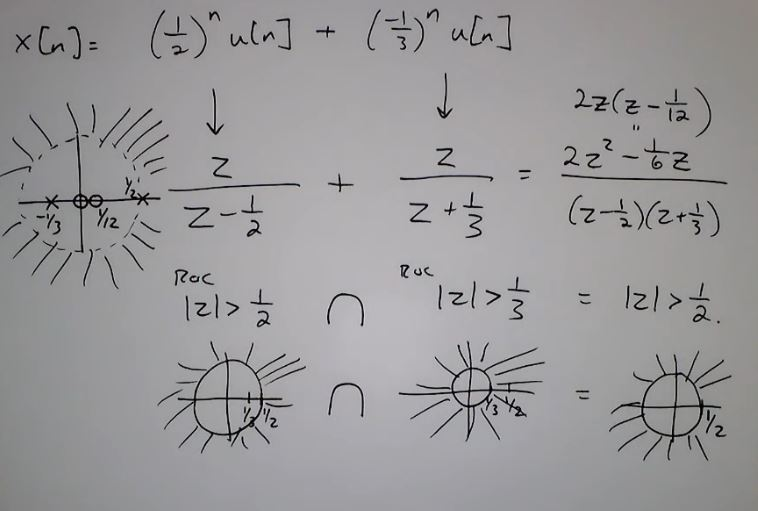
\includegraphics[scale=0.3]{Figures/z_transform/2_signals}
\label{fig:z_transform:summary_examples}
\end{figure}   
    
\item For $\lvert \, z \, \rvert \, > \, \displaystyle\frac{1}{3} \, \displaystyle \cap \, \lvert \, z \, \rvert \, > \, \displaystyle\frac{1}{2} \, \rightarrow \,  \lvert \, z \, \rvert \, > \, \displaystyle\frac{1}{2}$
    
\end{itemize}

\end{frame}


\subsubsection{Causal and Anticausal Signals}
\begin{frame}[t]{Causal and Anticausal Signals}

\begin{itemize}
    \item Now we take \textcolor{red}{causal and anticausal signals} $\leftrightarrow$ this give rise to a \textcolor{red}{double-sided signal} 
    
\begin{figure}[h]
\centering
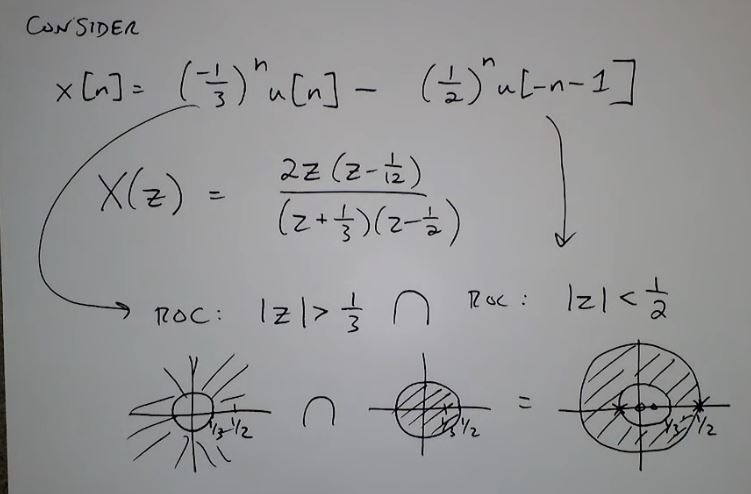
\includegraphics[scale=0.3]{Figures/z_transform/2_signals_b}
\label{fig:z_transform:summary_examples}
\end{figure}   
    
\item Notice that they have same $z$-transform, but different ROC region    
    
    
\end{itemize}

\end{frame}



\subsubsection{Summary Examples}
\begin{frame}[t,allowframebreaks]{Summary on Examples for Computing $Z$-Transform}

\begin{itemize}


\item Always Recall the rule: when using $X(z)$, we must \textcolor{red}{specify the region of convergence} for \textcolor{red}{unique correspondence} to a discrete time signal $x[k]$


\item Summary of Examples and their different region of convergence

\begin{figure}[h]
\centering
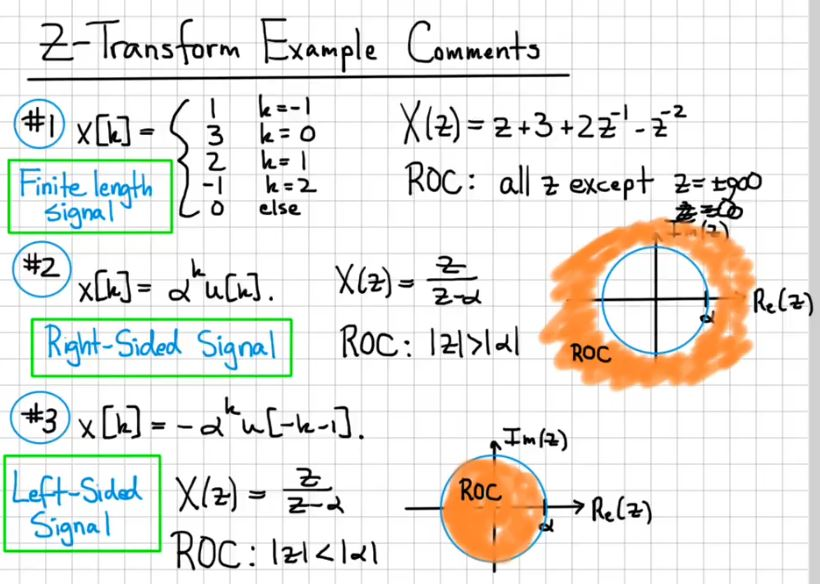
\includegraphics[scale=0.3]{Figures/z_transform/summary_examples}
\label{fig:z_transform:summary_examples}
\end{figure}

\newpage
\item Different Type of discrete time signal and their correspondent ROC

	\begin{enumerate}
	\item Finite duration  $\leftrightarrow$ all the z-plane except for 0 and $\pm \infty$
	
	\item Right sided signal $\leftrightarrow$ outside the circle
	
	\item Left sided signal $\leftrightarrow$ inside the circle
	\end{enumerate}


\item There is also 1 type of signals we didn't see: double sided signal (left and right side extension)

\item What we have done in this section is that we proved by examples different type of ROC for different type of signals

\item In the next slide, we do a general proof between ROC and the signal characteristics

\end{itemize}

\end{frame}


\subsubsection{Double Sided Signal}

\begin{frame}[t,allowframebreaks]{Double Sided Signal}

\begin{figure}[h]
\centering
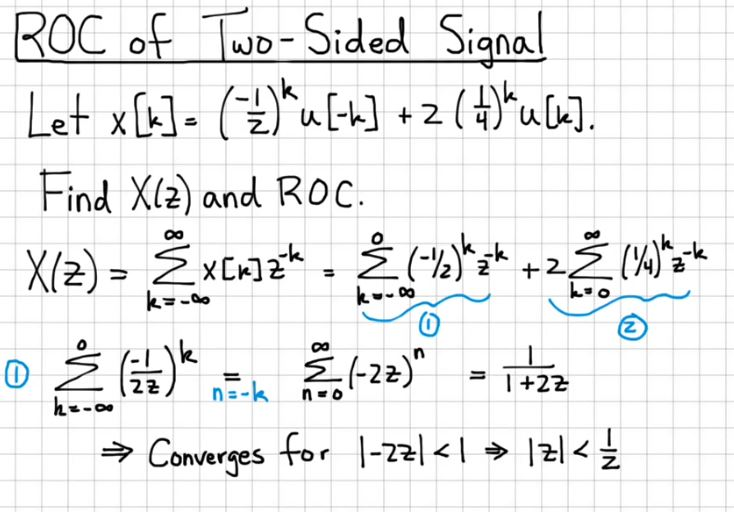
\includegraphics[scale=0.3]{Figures/z_transform/Double_Sided_negative}
\label{fig:z_transform:Double_Sided_negative}
\end{figure}

\begin{itemize}

\item We break the summation into negative part and positive part

\item In the term $\displaystyle\sum_{k \, = \, -\,\infty}^{0}$: we prefer to start the sum from 0, that's why we made the change of variable $ n \, = \, - \, k $

\end{itemize}

\newpage

\begin{figure}[h]
\centering
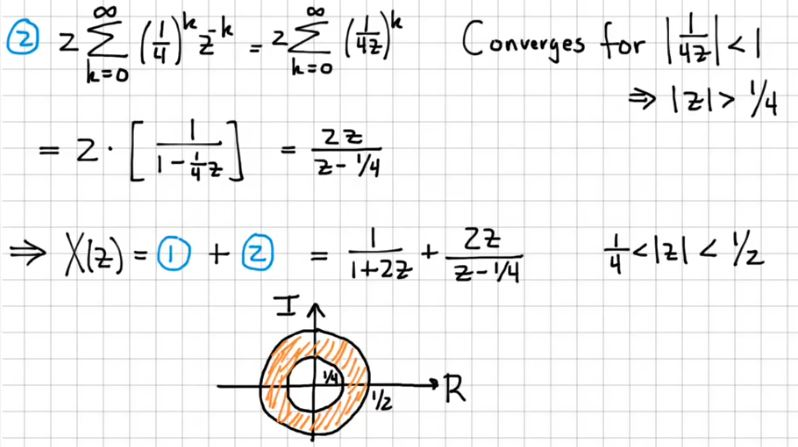
\includegraphics[scale=0.3]{Figures/z_transform/Double_Sided_positive}
\label{fig:z_transform:Double_Sided_positive}
\end{figure}

\begin{itemize}

\item We work the positive term here

\newpage
\item The ROC: it's the inequality from the negative term $\left(\,  |z| \, < \, \displaystyle\frac{1}{2}	  \,\right)$ and from the positive part $\left(\,  |z| \, > \, \displaystyle\frac{1}{4}	  \,\right)$

	\begin{itemize}
	\item This give us $ \displaystyle\frac{1}{4} < \, |z| \, < \, \displaystyle\frac{1}{2}	$
	
	\item The ROC is inside a \textcolor{red}{ring} for a \textcolor{red}{double sided discrete time signal} 
	\end{itemize}


\item Note: the circles should be plotted in dashed line and not solid, since the ROC inequality $ \displaystyle\frac{1}{4} < \, |z| \, < \, \displaystyle\frac{1}{2}	$ is \textcolor{red}{strictly less} and  \textcolor{red}{strictly above}

\end{itemize}

\end{frame}




\subsection{Theoretical Proof of Region of Convergence}
\begin{frame}[t,allowframebreaks]{Region of Convergence}

\begin{itemize}

\item To be done later


\end{itemize}


\end{frame}


\subsection{$Z$ Transform Properties}
\begin{frame}[t,allowframebreaks]{Example 1}

\begin{figure}[h]
\centering
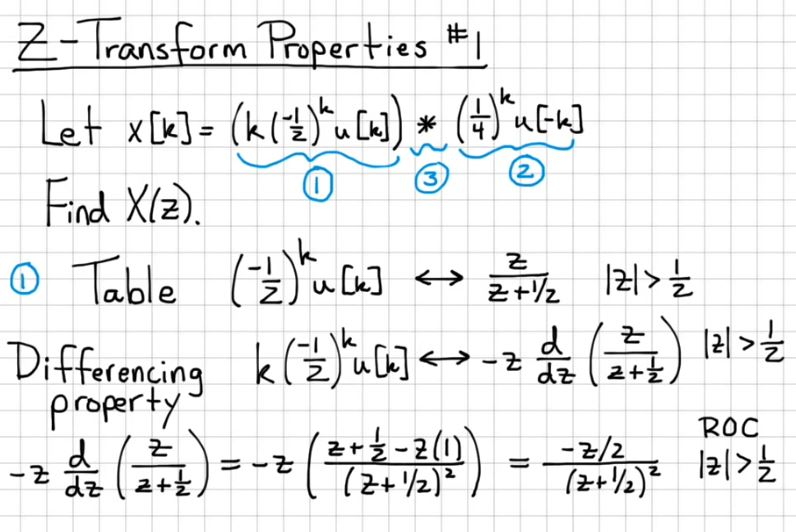
\includegraphics[scale=0.4]{Figures/z_transform/Properties_Example_1}
\label{fig:z_transform:Properties_Example_1}
\end{figure}


\begin{figure}[h]
\centering
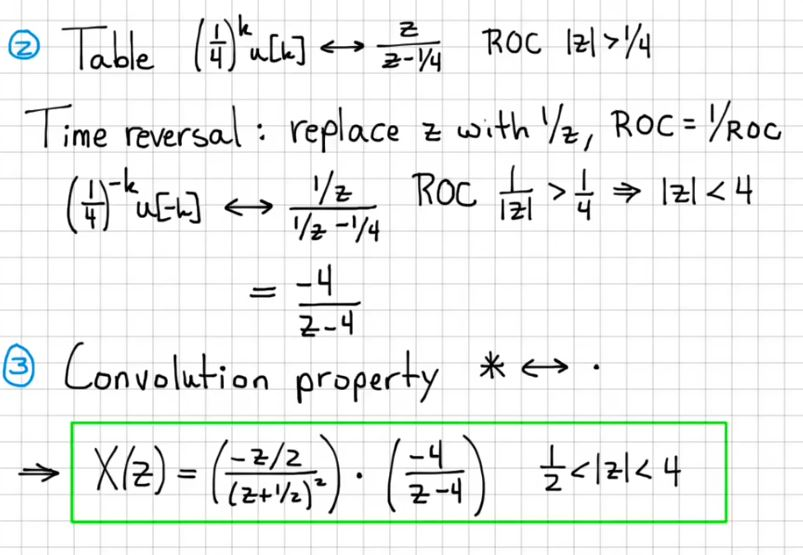
\includegraphics[scale=0.4]{Figures/z_transform/Properties_Example_1_2}
\label{fig:z_transform:Properties_Example_1_2}
\end{figure}


\end{frame}

\begin{frame}[t,allowframebreaks]{Example 2}

\begin{itemize}
\item Don't forget when using $z-$transform properties, keep track at what happen to the ROC for the final expression
\end{itemize}

\begin{figure}[h]
\centering
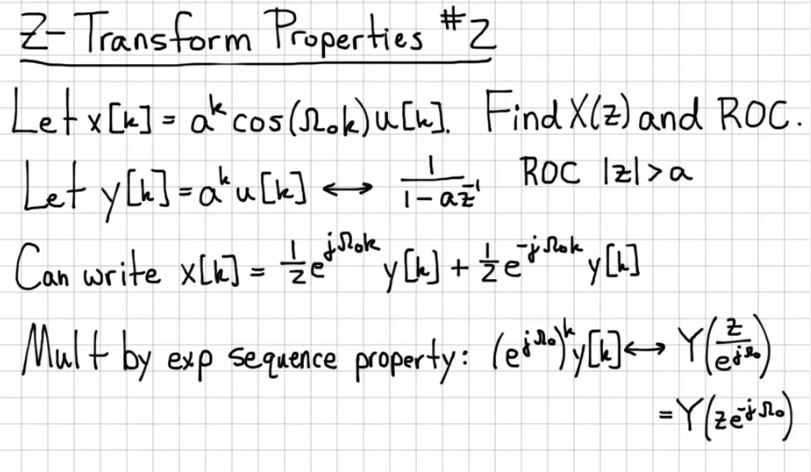
\includegraphics[scale=0.4]{Figures/z_transform/Properties_Example_2}
\label{fig:z_transform:Properties_Example_2}
\end{figure}

\begin{figure}[h]
\centering
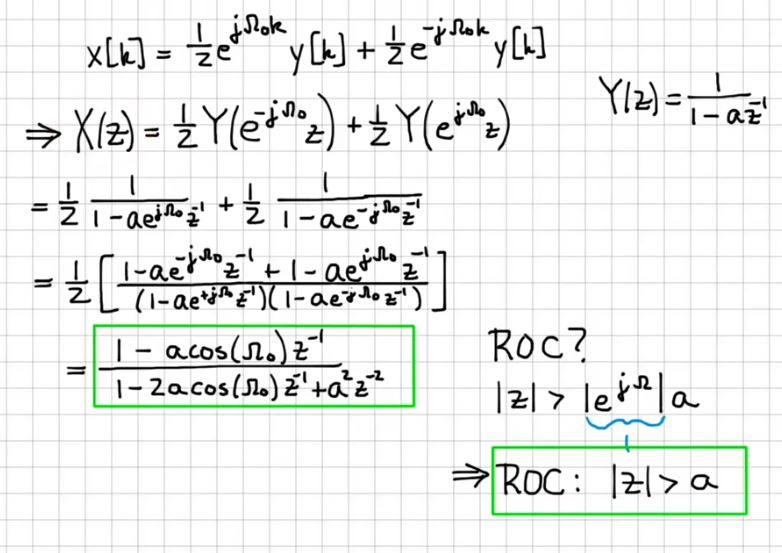
\includegraphics[scale=0.4]{Figures/z_transform/Properties_Example_2_2}
\label{fig:z_transform:Properties_Example_2_2}
\end{figure}


\end{frame}

\subsection{Pole-Zero Cancellation}

\begin{frame}[t,allowframebreaks]{Pole-Zero Cancellation}


\begin{itemize}
\item Given shown below
\end{itemize}

\begin{figure}[h]
\centering
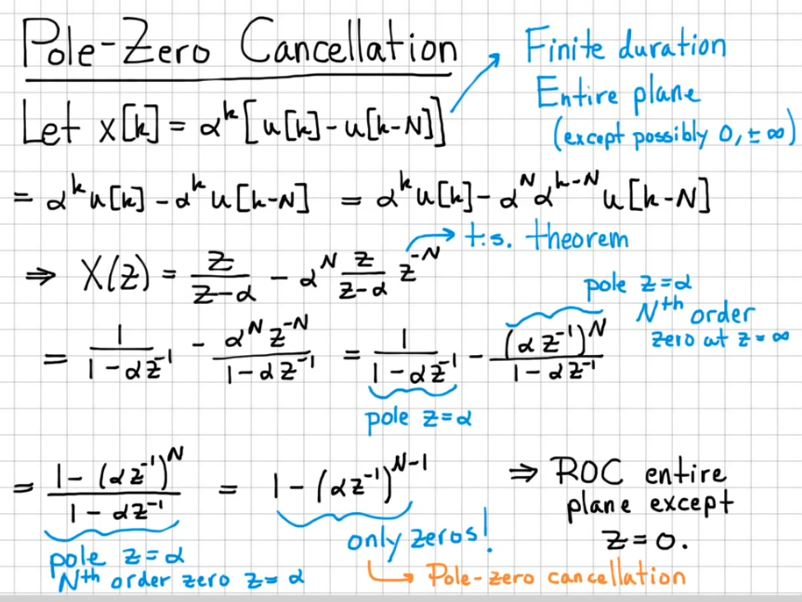
\includegraphics[scale=0.4]{Figures/z_transform/Pole_Zero_Cancellation}
\label{fig:z_transform:Pole_Zero_Cancellation}
\end{figure}

\newpage
\begin{itemize}

\item $u[k]$ turns on at $k \, = \, 0$

\item $u[k \, - \, N]$ turns on at $k \, = \, N$

\item If we subtract the 2 signals $u[k] \, - \, u[k \, - \, N]$ we get a \textcolor{red}{finite duration signal}

	\begin{itemize}
	\item \textcolor{red}{ROC} for finite duration signals is the \textcolor{red}{entire $z$ plane except for 0 and $\pm \, \infty$}
	\end{itemize}

\item $\alpha^k \ = \, \alpha^N \, \times \, \alpha^{k \, - \, N}$ so we can use the time shift theorem

\item When we have add the 2 terms $\displaystyle\frac{z}{z \, - \, \alpha}$ and $ \displaystyle\frac{z}{z \, - \, \alpha} \, z^{- \, N}$ to do simplification to the $X(z)$ expression, the zero of the numerator canceled out the pole of the denominator and we obtained finally $X(z) \, = \, 1 \, - \, \left(\, \alpha \, z^{-1} \,\right)^{N \,  - \, 1}$

	\begin{itemize}
	\item This final expression contains \textcolor{red}{only zero}
	
	\item The \textcolor{red}{ROC} has \textcolor{red}{expanded now} to contains also $\pm \, \infty$
	\end{itemize}

\item So as a conclusion, when we have some algebraic manipulation and combination of 2 expression, we may end up with an ROC bigger then what we have start in (for each expression)

\end{itemize}

\end{frame}



\subsection{Inverse $Z$-Transform}

\begin{frame}[t]{Inverse $Z$-Transform}

\begin{itemize}

\item Recall that the formal definition of the inverse of the $z$-transform:

\begin{definition}

The \textcolor{red}{inverse bilateral z-transform} of a $X[z]$ is:

\begin{equation}
x[k] \, = \, \displaystyle\frac{1}{2 \, \pi \, j} \displaystyle\oint X(z) \, z^{k \, - \, 1} \, dz
\end{equation}

\end{definition}


	\begin{itemize}
	\item We have a mathematical difficulty because we need to evaluate the \textcolor{red}{contour integral} $\displaystyle\oint$
	\end{itemize}


\item However we never use this explicit evaluation, instead we use some simpler method on practical expression of $X(z)$ encountered when dealing with discrete time LTI system:

	\begin{itemize}
	\item Ration of polynomials in function of $z^{- \, 1}$
	\end{itemize}

\end{itemize}

\end{frame}


\subsubsection{Partial Fraction Expansion (PFE)}

\begin{frame}[t]{Partial Fraction Expansion (PFE)}


\begin{itemize}

\item Ration of polynomials in function of $z^{- \, 1}$:

	\begin{equation}
	X(z) \, = \, \displaystyle\frac{B(z)}{A(z)}   \, = \, \displaystyle\frac{b_0 \, + \, b_1 \, z^{-1} \, + \, \cdots \, + \, b_M \, z^{- \, M}}{a_0 \, + \, a_1 \, z^{-1} \, + \, \cdots \, + \, a_N \, z^{- \, N}}
	\end{equation}

\item We would like to express the ration $\displaystyle\frac{B(z)}{A(z)}$ as \textcolor{red}{linear combination of $1^{\mathrm{st}}$ order terms}:

	\begin{equation}
	X(z) \, = \, \displaystyle\sum\limits_{i \, = \, 1}^N\frac{A_i}{1 \, - \, d_i \, z^{-1}}
	\label{Eq:z_transform:first_order_terms}
	\end{equation}
	
	\begin{itemize}
	\item The nice thing about equation (\autoref{Eq:z_transform:first_order_terms}) is we know their time domain expression
	\end{itemize}

\end{itemize}

\end{frame}


\begin{frame}[t]{ROC Ambiguity}

\begin{itemize}

\item However, recall that when specifying \textcolor{red}{$z$-transform}, we \textcolor{red}{always} need to \textcolor{red}{specify the ROC}

	\begin{itemize}
	\item Because 1 $X(z)$ can have several time domain expression \textcolor{red}{but always different (unique) ROC}	
	\end{itemize}

\item Concerning the $1^{\mathrm{st}}$ order $\frac{A_i}{1 \, - \, d_i \, z^{-1}}$ term, in which we have 2 choice as inverse $z$-transform:

	\begin{enumerate}
	\item $ \displaystyle\frac{A_i}{1 \, - \, d_i \, z^{-1}} A_i \, \leftrightarrow \, (d_i)^k \, \underbrace{u[k] }_{\text{right sided signal}} $ for an ROC $\underbrace{|z| \, > \, d_i}_{\text{Radius $>$ pole}}$
	
	\item  $ \displaystyle\frac{A_i}{1 \, - \, d_i \, z^{-1}} \, \leftrightarrow \, A_i \, (d_i)^k \, \underbrace{ u[\, -k \, - \, 1 \,] }_{\text{left sided signal}}\, $ for an ROC $|z| \, < \, d_i$
	\end{enumerate}

\item To \textcolor{red}{choose} the \textcolor{red}{correct discrete time domain expression}, we always need to \textcolor{red}{include} the \textcolor{red}{initial ROC of $X(z)$ before expansion}

	\begin{itemize}
	\item An example in the next slides will clear this up.
	\end{itemize}
\end{itemize}

\end{frame}


\begin{frame}[t,allowframebreaks]{Examples}

\begin{figure}[h]
\centering
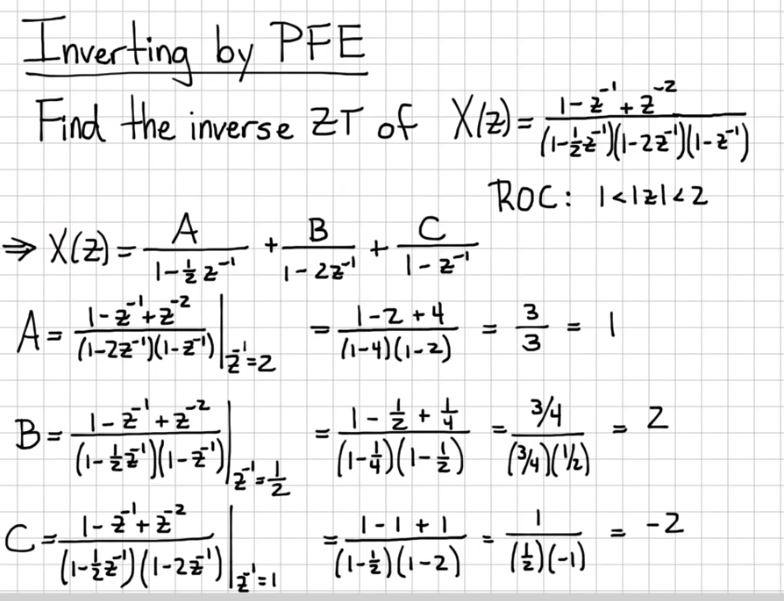
\includegraphics[scale=0.3]{Figures/z_transform/PFE_Examples_1}
\label{fig:z_transform:PFE_Examples_1}
\end{figure}

\begin{itemize}

\item The initial ROC of $X(z)$ before PFE is $ 1 \, < \, |z| \, < \, 2$

\end{itemize}

\newpage

\begin{figure}[h]
\centering
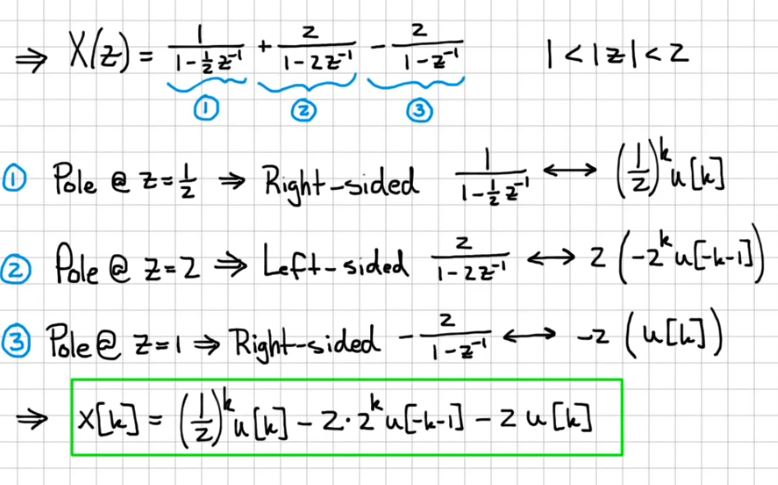
\includegraphics[scale=0.4]{Figures/z_transform/PFE_Examples_1_2}
\label{fig:z_transform:PFE_Examples_1_2}
\end{figure}

\begin{itemize}

\item Any ROC for terms 1,2 and 3 must include $ 1 \, < \, |z| \, < \, 2$

\item Work for the ROC of each term independently 

\end{itemize}



\end{frame}

\begin{frame}[t]{Unknown Initial ROC}

\begin{itemize}
\item In the previous example, we were given the ROC of $X(z)$: $ 1 \, < \, |z| \, < \, 2$
 
\item But what if we don't have it?

\item We can \textcolor{red}{use the information we know about the signals/system we have}:

	\begin{itemize}
	\item If we know we work with \textcolor{red}{stable system} $\leftrightarrow$ DTFT exist $\leftrightarrow$ \textcolor{red}{ROC} must \textcolor{red}{include the unit circle}
	
		\begin{itemize}
		\item Signals can be left side of right side
		\end{itemize}
	
	\item If we work with \textcolor{red}{causal signals}  $\leftrightarrow$ chose the \textcolor{red}{right sided inverse} for each term 
\end{itemize}	 
 
\end{itemize}


\end{frame}


\subsubsection{Long Division Inversion}

\begin{frame}[t]{Long Division Inversion}

\begin{itemize}

\item Partial fraction expansion (PFE) is one way we can do inverse $z$-transform

\item Another way we can do  inverse $z$-transform is \textcolor{red}{long division method}, which can be done when we have \textcolor{red}{1-sided signal}

	\begin{enumerate}
	\item if ROC \textcolor{red}{inside the unite circle} $\leftrightarrow \, |z| \, < \, a \leftrightarrow \, \text{right sided signal} \, \rightarrow$ we get a \textcolor{red}{sequence of positive power} of $z$ 
	
		\item if ROC \textcolor{red}{outside the unite circle} $\leftrightarrow \, |z| \, > \, a \, \leftrightarrow \, \text{left sided signal} \, \rightarrow$ we get a \textcolor{red}{sequence of negative power} of $z^{-1}$ 
	\end{enumerate}

\end{itemize}

\end{frame}

\begin{frame}[t]{Long Division Example 1: Right Sided Signal}

\begin{figure}[h]
\centering
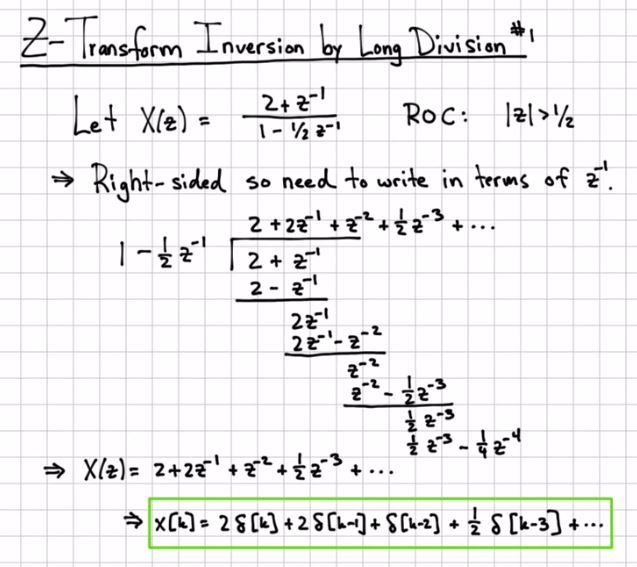
\includegraphics[scale=0.4]{Figures/z_transform/long_division_Examples_1}
\label{fig:z_transform:long_division_Examples_1}
\end{figure}

\begin{itemize}
\item $x[k]$: we have a part of the signal

\item This type of methods is useful when we need a part of the signal and not all of its components

	\begin{itemize}
	\item Example: Working with initial conditions with finite difference equations
	\end{itemize}
\end{itemize}

\end{frame}

\begin{frame}[t]{Long Division Example 2: Left Sided Signal}

\begin{figure}[h]
\centering
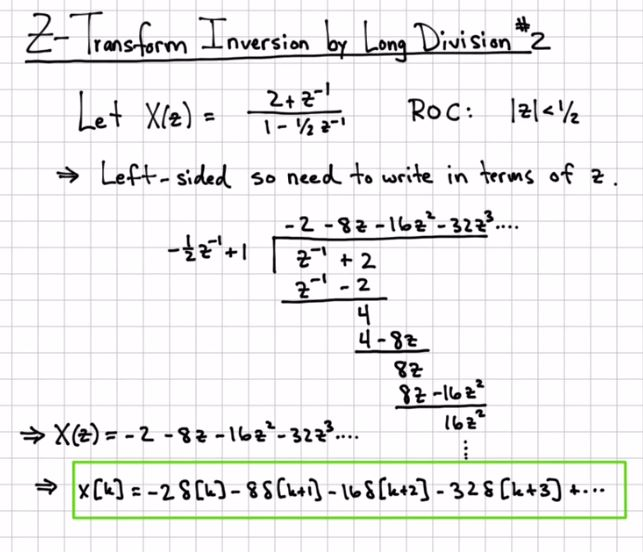
\includegraphics[scale=0.4]{Figures/z_transform/long_division_Examples_2}
\label{fig:z_transform:long_division_Examples_2}
\end{figure}


\end{frame}



\subsection{System Analysis and Transfer Function}

\begin{frame}[t]{System Analysis and Transfer Function}

\begin{block}{Transfer Function}
The input-output behavior of a discrete-time LTI system is
determined by the \textcolor{red}{system transfer function}

\begin{equation}
H(z) \, = \, \displaystyle\frac{Y(z)}{X(z)}
\end{equation}

\end{block}

\end{frame}


\subsubsection{Examples}

\begin{frame}[t,allowframebreaks]{Example of Finding $H(z)$ and $h(n)$}

\begin{figure}[h]
\centering
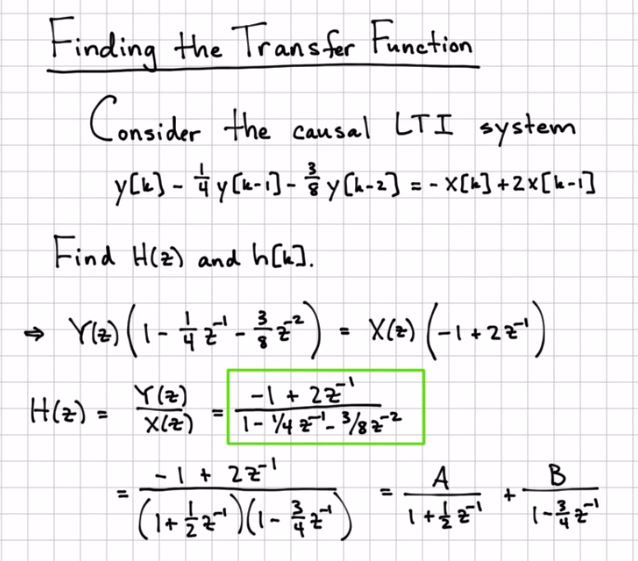
\includegraphics[scale=0.4]{Figures/z_transform/Example_transfer_function_1_1}
\label{fig:z_transform:Example_transfer_function_1_1}
\end{figure}

\newpage
\begin{figure}[h]
\centering
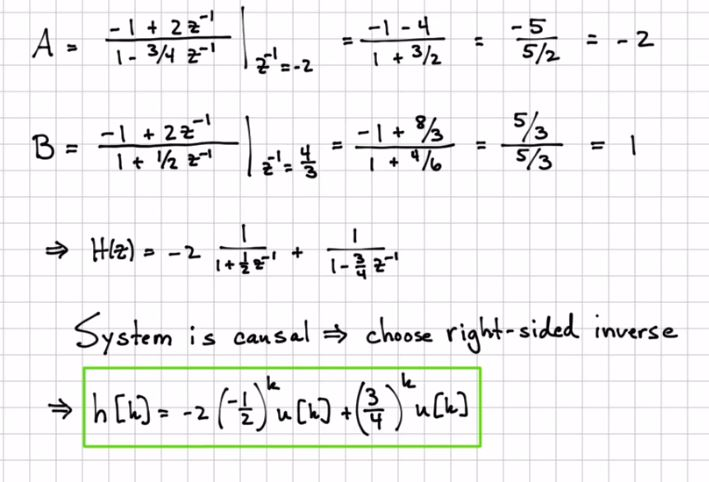
\includegraphics[scale=0.4]{Figures/z_transform/Example_transfer_function_1_2}
\label{fig:z_transform:Example_transfer_function_1_2}
\end{figure}

\end{frame}


\begin{frame}[t]{Example of Finding Difference Equation}

\begin{figure}[h]
\centering
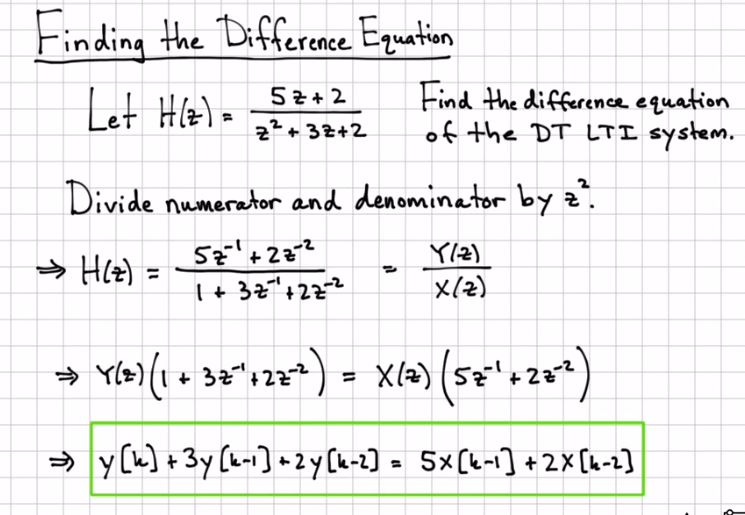
\includegraphics[scale=0.4]{Figures/z_transform/Example_Difference_Equation}
\label{fig:z_transform:Example_Difference_Equation}
\end{figure}


\end{frame}

\begin{frame}[t,allowframebreaks]{System Identification}

\begin{figure}[h]
\centering
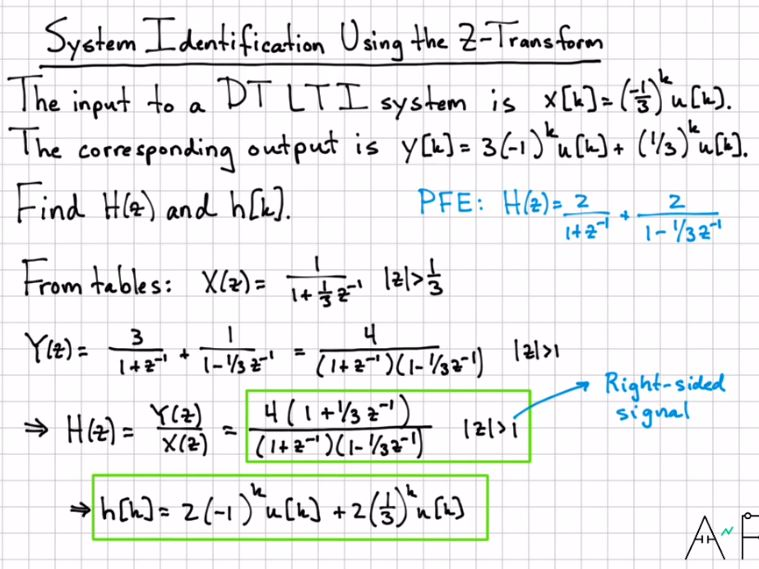
\includegraphics[scale=0.4]{Figures/z_transform/system_identification}
\label{fig:z_transform:system_identification}
\end{figure}


\begin{itemize}

\item Be aware that we need to \textcolor{red}{keep track the ROC} when computing $H(z)$ using $Y(z)$ and $X(z)$:

	\begin{itemize}
	\item $|z| \, > \, \displaystyle\frac{1}{3}$ and $|z| \, > \, 1$
	
	\item The \textcolor{red}{common area} is $|z| \, > \, 1$
	\end{itemize}

\item When solving for $h(n)$ by \textcolor{red}{taking inverse of $H(z)$}: need to be careful \textcolor{red}{which time domain signal to choose}: \textcolor{red}{right} or \textcolor{red}{left} sided

	\begin{itemize}
	\item But since ROC for $H(z)$ is $|z| \, > \, 1 \rightarrow$ we choose right sided signals
	\end{itemize}

\end{itemize}


\end{frame}


\subsubsection{Causality and Stability}

\begin{frame}[t]{Causality and Stability}

\begin{itemize}

\item In this section, we will \textcolor{red}{examine the transfer function} and try to learn what \textcolor{red}{information} we can get about the \textcolor{red}{behavior} of the \textcolor{red}{system}


\item These information will be the governed by the \textcolor{red}{location of the poles of the system}

\item Location of the pole if it is outside the unite circle, we get either:

	\begin{enumerate}
	\item A decaying exponential $\leftrightarrow$ Non-causal but stable
	
	\item An increasing right sided exponential $\leftrightarrow$ Causal but not stable	
	\end{enumerate}

\item To ensure \textcolor{red}{stability and causality}: \textcolor{red}{poles} must be \textcolor{red}{inside the unit circle}

\end{itemize}

\end{frame}



\begin{frame}[t]{Example: Find $h[k]$ for a Stable System}

\begin{figure}[h]
\centering
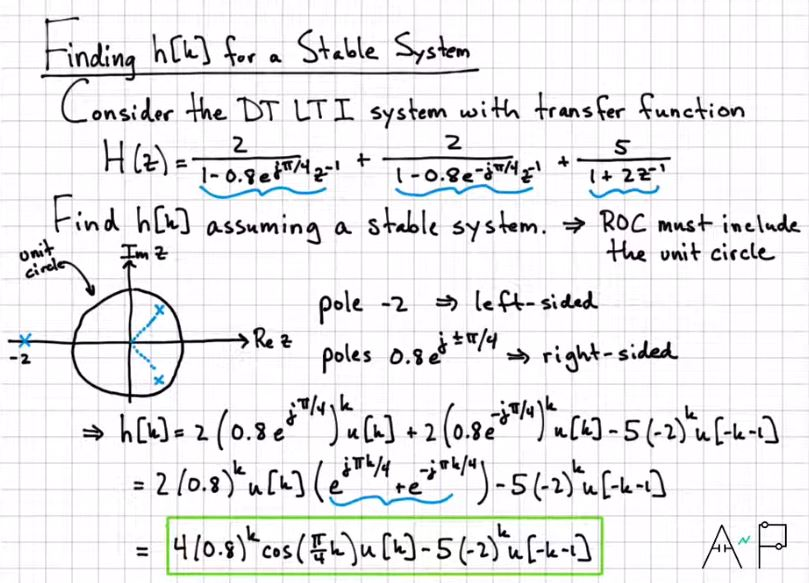
\includegraphics[scale=0.4]{Figures/z_transform/impulse_response_stable_system_example}
\label{fig:z_transform:impulse_response_stable_system_example}
\end{figure}


\end{frame}

\begin{frame}[t]{Example: Find $h[k]$ for a Stable System}

\begin{itemize}

\item Since we are assuming that the system is stable, the ROC must include the unit circle

	\begin{itemize}
	\item So we need to be aware when taking $z$-inverse for each of the term in $H(z)$ expression
	\end{itemize}

\item For the pole $= \, - \, 2$: we need to include the unit circle so we choose a left sided signal

\item The other complex poles: they are inside the unit circle, and want to include the unit circle, so we take the ROC outside and hence we need a right sided signal

\end{itemize}


\end{frame}


\begin{frame}[t]{Example: Find $h[k]$ for a Causal System}

\begin{figure}[h]
\centering
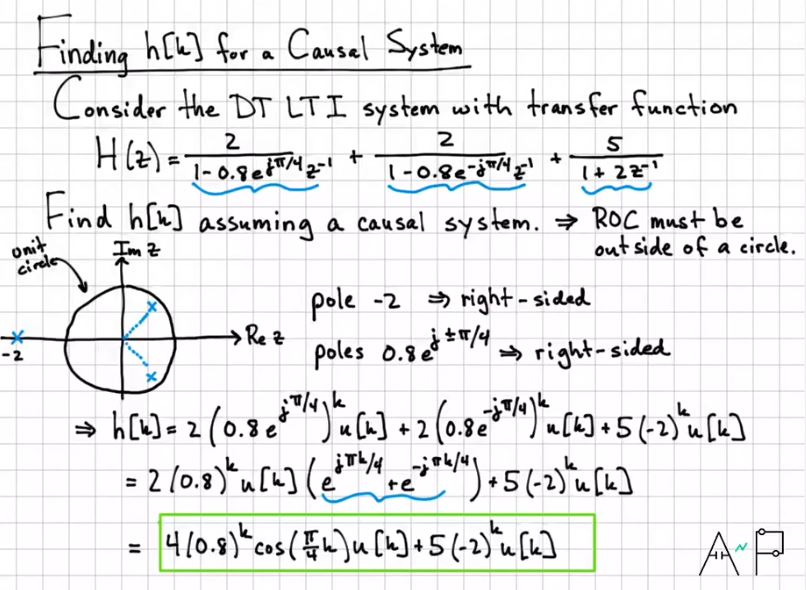
\includegraphics[scale=0.4]{Figures/z_transform/impulse_response_causal_system_example}
\label{fig:z_transform:impulse_response_causal_system_example}
\end{figure}

\end{frame}

\begin{frame}[t]{Example: Find $h[k]$ for a Causal System}

\begin{itemize}

\item For a \textcolor{red}{causal system}, things are easier

\item The \textcolor{red}{ROC} need to be \textcolor{red}{outside the unit circle}

	\begin{itemize}
	\item So for every pole we have, we choose a right sided signal 
	\end{itemize}

\end{itemize}

\end{frame}


\subsection{Inverse Linear System and Minimum Phase}

\begin{frame}[t]{Inverse Linear System and Minimum Phase}

\begin{itemize}

\item Suppose we want to compute the transfer function that \textcolor{red}{undo the effect} of our original system $h[n]$

\item By definition, such an inverse system if we convolve its impulse response $h_{\text{inv}}[n]$ with $h[n]$ we obtain a pulse $\delta[n]$

\begin{equation}
(\,h_{\text{inv}} \, \star \, h \,)[n] \, = \, \delta[n]
\end{equation}

\item Taking this definition into the $z$-domain we have:

\begin{equation}
H_{\text{inv}}(z) \, \times \, H(z) \, = \, 1 
\end{equation}

\end{itemize}

\begin{block}{Definition}
The \textcolor{red}{Inverse System Transfer Function} is the inverse the transfer function of the original system

	\begin{equation}
	H_{\text{inv}}(z) \, = \, \displaystyle\frac{1}{H(z)}
	\end{equation}
\end{block}


\end{frame}

\begin{frame}[t]{Causality and Stability Inverse Linear System and Minimum Phase}

\begin{itemize}

\item When designing real word system, we want them to be \textcolor{red}{causal} and \textcolor{red}{stable}

\item Dealing with \textcolor{red}{$H_{\text{inv}}(z)$}, they have the \textcolor{red}{flipped poles and zeros of $H(z)$}

\item So if we want $H_{\text{inv}}(z)$ to be causal and stable, the \textcolor{red}{poles} and \textcolor{red}{zeros} of $H(z)$ must be \textcolor{red}{inside the unit circle}

\end{itemize}

\begin{block}{Definition}

A system $H(z)$ having \textcolor{red}{all its poles and zeros inside the unit circle} is called a \textcolor{red}{minimum phase system}

\end{block}

\end{frame}



\begin{frame}[t]{Example}

\begin{figure}[h]
\centering
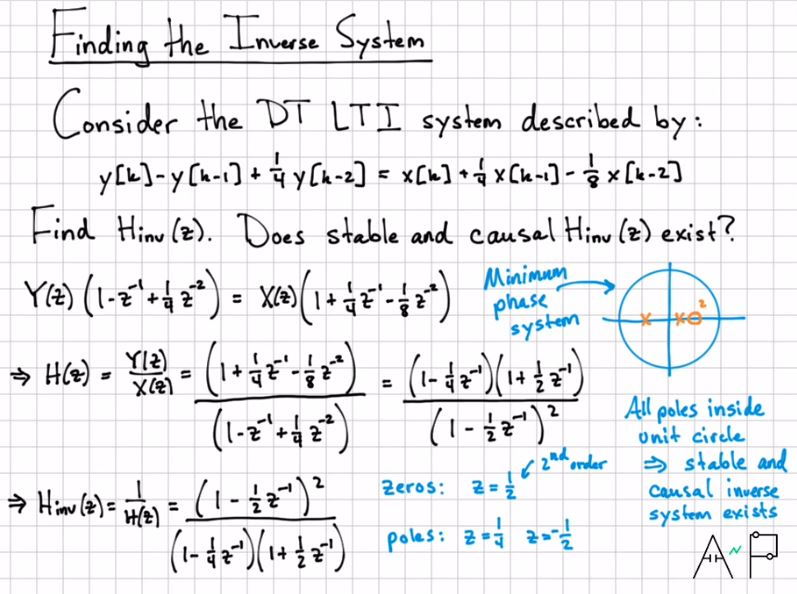
\includegraphics[scale=0.4]{Figures/z_transform/inverse_linear_sytem_example}
\label{fig:z_transform:inverse_linear_sytem_example}
\end{figure}


\end{frame}



\subsection{Frequency Response $H(\omega_d)$}

\begin{frame}[t]{Frequency Response $H(\omega_d)$ form Poles and Zeros}

\begin{itemize}

\item Now in this section we learn how to \textcolor{red}{sketch frequency response} $H(\omega_d)$ by \textcolor{red}{tracking} the \textcolor{red}{poles} and \textcolor{red}{zeros} \textcolor{red}{from the unit circle in the $z$-plane}

\item It is true that we have some programming tools that can do this for us, but be able to do this by hand will give us more understanding about the relation between the $z$-transform tools and the frequency response $H(\omega_d)$ in the DTFT domain

\end{itemize}

\end{frame}

\begin{frame}[t,allowframebreaks]{Computation}

\begin{itemize}

\item We know that we can obtain DTFT expression by letting $z \, = \, e^{j \, \omega_d}$

\item $H(z)$ is the product of zeros over the product of poles

\begin{equation}
H(z) \, = \, \displaystyle\frac{( \, z \, - \, z_1 \,) \, \times \, ( \, z \, - \, z_2 \,) \, \times \, \cdots \, \times \, ( \, z \, - \, z_n \,)}{( \, z \, - \, p_1 \,) \, \times \,( \, z \, - \, p_2 \,) \, \times \, \cdots \, \times \,( \, z \, - \, p_n \,)}
\end{equation} 

\item We let $z \, = \,  e^{j \, \omega_d}$ and make the substitution in $H(z)$:

\begin{equation}
H(\omega_d) \, = \, \displaystyle\frac{( \,  e^{j \, \omega_d} \, - \, z_1 \,) \, \times \, ( \,  e^{j \, \omega_d} \, - \, z_2 \,) \, \times \, \cdots \, \times \, ( \,  e^{j \, \omega_d} \, - \, z_n \,)}{( \,  e^{j \, \omega_d} \, - \, p_1 \,) \, \times \,( \,  e^{j \, \omega_d} \, - \, p_2 \,) \, \times \, \cdots \, \times \,( \,  e^{j \, \omega_d} \, - \, p_n \,)}
\label{Eq:z_transfomr:freq_response_2}
\end{equation} 

\newpage

\item 3 quantities are the key in equation \autoref{Eq:z_transfomr:freq_response_2}:

	\begin{enumerate}
	\item The quantity $e^{j \, \omega_d}$ is on the unit circle
	
	\item The quantity $ e^{j \, \omega_d} \, - \, z_i$ is a vector from $z_i \, \rightarrow \, e^{j \, \omega_d}$
	
	
	\item The quantity $ e^{j \, \omega_d} \, - \, p_i$ is a vector from $p_i \, \rightarrow \, e^{j \, \omega_d}$
	\end{enumerate}


\item So we can write these vectors using polar expression as:

\begin{equation}
\begin{array}{rcl}
r_i \, e^{j \, \phi_i} \, = \, e^{j \, \omega_d} \, - \, z_i \\
d_i \, e^{j \, \theta_i} \, =  e^{j \, \omega_d} \, - \, p_i 
\end{array}
\label{Eq:z_transfomr:freq_response_3}
\end{equation}

\item Putting equation (\autoref{Eq:z_transfomr:freq_response_3}) in equation (\autoref{Eq:z_transfomr:freq_response_2})

\begin{equation}
\begin{array}{rcl}
H(\omega_d) \, &=& \, \displaystyle\frac{( \, r_i \, e^{j \, \phi_1} \,) \, \times \, ( \,  r_i \, e^{j \, \phi_2}\,) \, \times \, \cdots \, \times \, ( \, r_i \, e^{j \, \phi_n} \,)}{( \,  d_i \, e^{j \, \theta_1} \,) \, \times \,( \, d_i \, e^{j \, \theta_2} \,) \, \times \, \cdots \, \times \,( \,  d_i \, e^{j \, \theta_n} \,)} \\ \\
		&=& \, \displaystyle\frac{r_1 \, r_2 \, \cdots \, r_n}{d_1 \, d_2 \, \cdots \, d_n} \, \times \,  \\
		&&  \text{exp} \, (\, j \, \left[ \,  ( \phi_1 \, + \, \phi_2 \, \cdots \, \phi_n ) \, - \, (\, \theta_1 \, + \, \theta_2 \, + \, \cdots \, + \, \theta_n \,) \,\right] )
\end{array}
\end{equation}

\end{itemize}


\end{frame}

\begin{frame}[t]{Formula for Amplitude and Phase Response}

\begin{equation}
\begin{array}{rcl}
\lvert\, H(\omega_d) \, \rvert \, &=& \, \displaystyle\frac{r_1 \, r_2 \, \cdots \, r_n}{d_1 \, d_2 \, \cdots \, d_n} \\ \\
 \phase{H(\omega_d)} \, &=& \, (\, \phi_1 \, + \, \phi_2 \, \cdots \, \phi_n ) \, - \, (\, \theta_1 \, + \, \theta_2 \, + \, \cdots \, + \, \theta_n \,) \\
 		&=& \text{Sum of zeros angles to } e^{j \omega_d} \, - \,  \text{Sum of poles angles to } e^{j \omega_d}
\end{array}
\end{equation}

\end{frame}


\begin{frame}[t]{Example}

\begin{figure}[h]
\centering
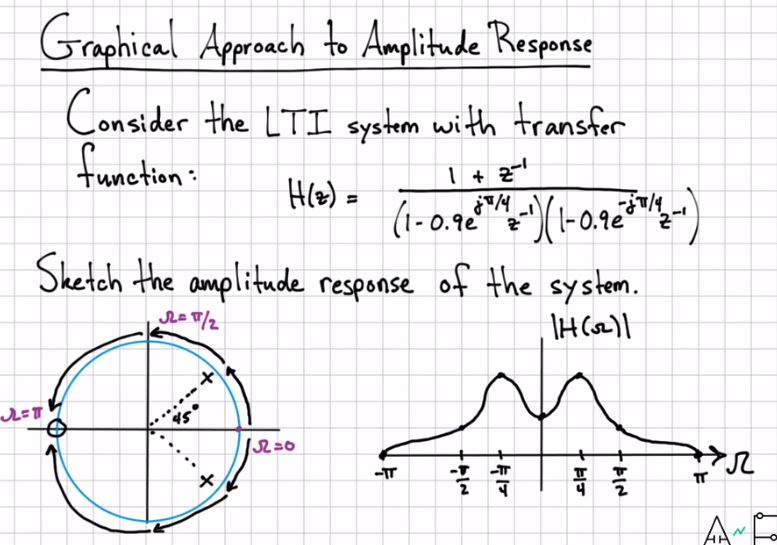
\includegraphics[scale=0.4]{Figures/z_transform/frequency_response_approximate_sketch_example}
\label{fig:z_transform:frequency_response_approximate_sketch_example}
\end{figure}


\end{frame}



\subsection{Unilateral $Z$-Transform}

\begin{frame}[t]{Introduction}

\begin{itemize}

\item Unilateral $Z$-Transform are useful if we want to \textcolor{red}{restrict} ourselves to be working with \textcolor{red}{causal signals/systems}

\item Advantage:

	\begin{itemize}
	\item Don't need to worry about the ROC $\leftrightarrow$ since the \textcolor{red}{signals} are \textcolor{red}{causal}, we know that the \textcolor{red}{ROC} will be \textcolor{red}{something outside the unite circle}
	
	\item Help us solved difference equation
	\end{itemize}



\begin{block}{Definition}

The \textcolor{red}{Unilateral $Z$-Transform} of the discrete time signal $x[k]$ is:

\begin{equation}
X(z) \, = \, \displaystyle\sum_{k \, = \, 0}^{+ \, \infty} x[k] \, z^{-k}
\end{equation}

\end{block}


\end{itemize}

\end{frame}


\subsubsection{Time Shift Properties}

\begin{frame}[t]{Time Shift Properties}

\begin{itemize}

\item All the properties of the bilateral $Z$-transform are the same for the unilateral $Z$-transform except when doing time shift

\item 2 types of time shift can be done for $N \, > \, 0 \in \, \mathbb{N}$:

	\begin{enumerate}
	\item Delay $\leftrightarrow$ shifting to the right $\leftrightarrow \, x[k \,-\, N] \, u[k]$ 
	
	\item Time Advance $\leftrightarrow$ shifting to the left $\leftrightarrow \, x[k \,+\, N] \, u[k]$ 
	\end{enumerate}

\item When plug in the 2 time shifted signal into the unilateral $Z$-transform definition we get:

\begin{equation}
\begin{array}{rcl}
x[k \,-\, N] \, u[k] \, &\leftrightarrow& \, z^{-N} \, X(z) \, + \, z^{-N} \,   \displaystyle\sum_{k \, = \, 1}^{N} x[\, -\,k \,] \, z^k  \\ \\
x[k \,+ \, N] \, u[k] \, &\leftrightarrow& \, z^N \, X(z) \, - \, z^N \,   \displaystyle\sum_{k \, = \, 0}^{N \ - \, 1} x[k] \, z^{-k}
\end{array}
\end{equation} 

\end{itemize}

\end{frame}

\begin{frame}[t]{Time Delay Pattern}

\begin{itemize}

\item $N \, = \, 1$

\begin{equation*}
x[k \, - \, 1] \, u[k] \,\leftrightarrow \,  z^{-1} \, X(z) \, + \, x[-1]
\end{equation*}

\item $N \, = \, 2$

\begin{equation*}
x[k \, - \, 2] \, u[k] \,\leftrightarrow \,  z^{-2} \, X(z)\, + \, z^{-1} \, x[-1] \, + \, x[-2]
\end{equation*}


\item $N \, = \, 3$

\begin{equation*}
x[k \, - \, 1] \, u[k] \,\leftrightarrow \,  z^{-3} \, X(z)\, + \, z^{-2} \, x[-1] \, + \, z^{-1}\, x[-2] \, + \, x[-3]
\end{equation*}

\end{itemize}

\end{frame}

\begin{frame}[t]{Observation in Time Delay Pattern}

\begin{itemize}

\item Notice that in each term for any $N$ value, the sum in each term is equal to $N$

\item Example for $N \, = \, 2$

	\begin{itemize}
	\item \begin{equation*}
x[k \, - \, 2] \, u[k] \,\leftrightarrow \,  z^{-2} \, X(z)\, + \, z^{-1} \, x[-1] \, + \, x[-2]
\end{equation*}

	\item The term $z^{-1} \, x[-1] $: we have 1 and 1 give 2
	\end{itemize}

\item Same for the terms in case of $N \, = \, 3$

	\begin{itemize}
	\item $z^{-1} \, x[-2] $: 1 and 2 give 3
	
	\item $z^{-2} \, x[-1] $: 2 and 1 give 3
	\end{itemize}

\item Same concept exist in time advance pattern

\end{itemize}

\end{frame}

\begin{frame}[t]{Time Advance Pattern}

\begin{itemize}

\item $N \, = \, 1$

\begin{equation*}
x[k \, + \, 1] \, u[k] \,\leftrightarrow \,  z \, X(z) \, - \, z \, x[0]
\end{equation*}

\item $N \, = \, 2$

\begin{equation*}
x[k \, + \, 2] \, u[k] \,\leftrightarrow \,  z^{2} \, X(z)\, - \, z^{2} \, x[0] \, - \,z \, x[	1]
\end{equation*}


\item $N \, = \, 3$

\begin{equation*}
x[k \, + \, 3] \, u[k] \,\leftrightarrow \,  z^{3} \, X(z)\, - \, z^{3} \, x[0] \, - \, z^{2}\, x[1] \, - \, z\, x[2]
\end{equation*}

\end{itemize}

\end{frame}


%**************************************************
%**************************************************
%**************************************************

\section{Convolution and Correlation}
\label{Chap:Convolution_Correlation}
\begin{frame}[t]{Chapter \autoref{Chap:Convolution_Correlation}}
\tableofcontents[sections= \value{section}]
\end{frame}

\begin{frame}[t,allowframebreaks]{Convolution}



\end{frame}


\begin{frame}[t,allowframebreaks]{Circular Convolution}



\end{frame}

%**************************************************
%**************************************************
%**************************************************

\section{Fast Fourier Transform}
\label{Chap:FFT}
\begin{frame}[t]{Chapter \autoref{Chap:FFT}}
\tableofcontents[sections= \value{section}]
\end{frame}

\begin{frame}[t,allowframebreaks]{Introduction to FFT}

\begin{itemize}

\item The FFT is an \textcolor{red}{algorithm} which implements the DFT in an efficient manner


\item Put figure of comparison

	\begin{itemize}
	\item When $\text{log}_{10}(N) \, = \, 2$ which means that $N \, = \, 100$ samples, there is no a big difference between the DFT and the FFT
	
	\item As $\text{log}_{10}(N)$ increase, like at 6 (so $N$ is 1 million sample), the gap in the number of operation increase allot 
	\end{itemize}

\end{itemize}


\end{frame}

\begin{frame}[t,allowframebreaks]{FFT Algorithm details}

\begin{itemize}

\item We can compute 2 points of the DFT using only 1 multiplication

\item Many algorithms used in FFT, we look at the one so called \textcolor{red}{decimation in time}


\end{itemize}


\end{frame}



%**************************************************
%**************************************************
%**************************************************

\section{Analysis and Simulation: Sampling and Frequency Analysis}
\begin{frame}[t,allowframebreaks]{Table of contents}
\tableofcontents[currentsection,hidesubsections]
\end{frame}


\subsection{Aliasing}
\begin{frame}[t,allowframebreaks]{Sampling a Cos wave and Aliasing Frequency}

\begin{figure}[h]
\centering
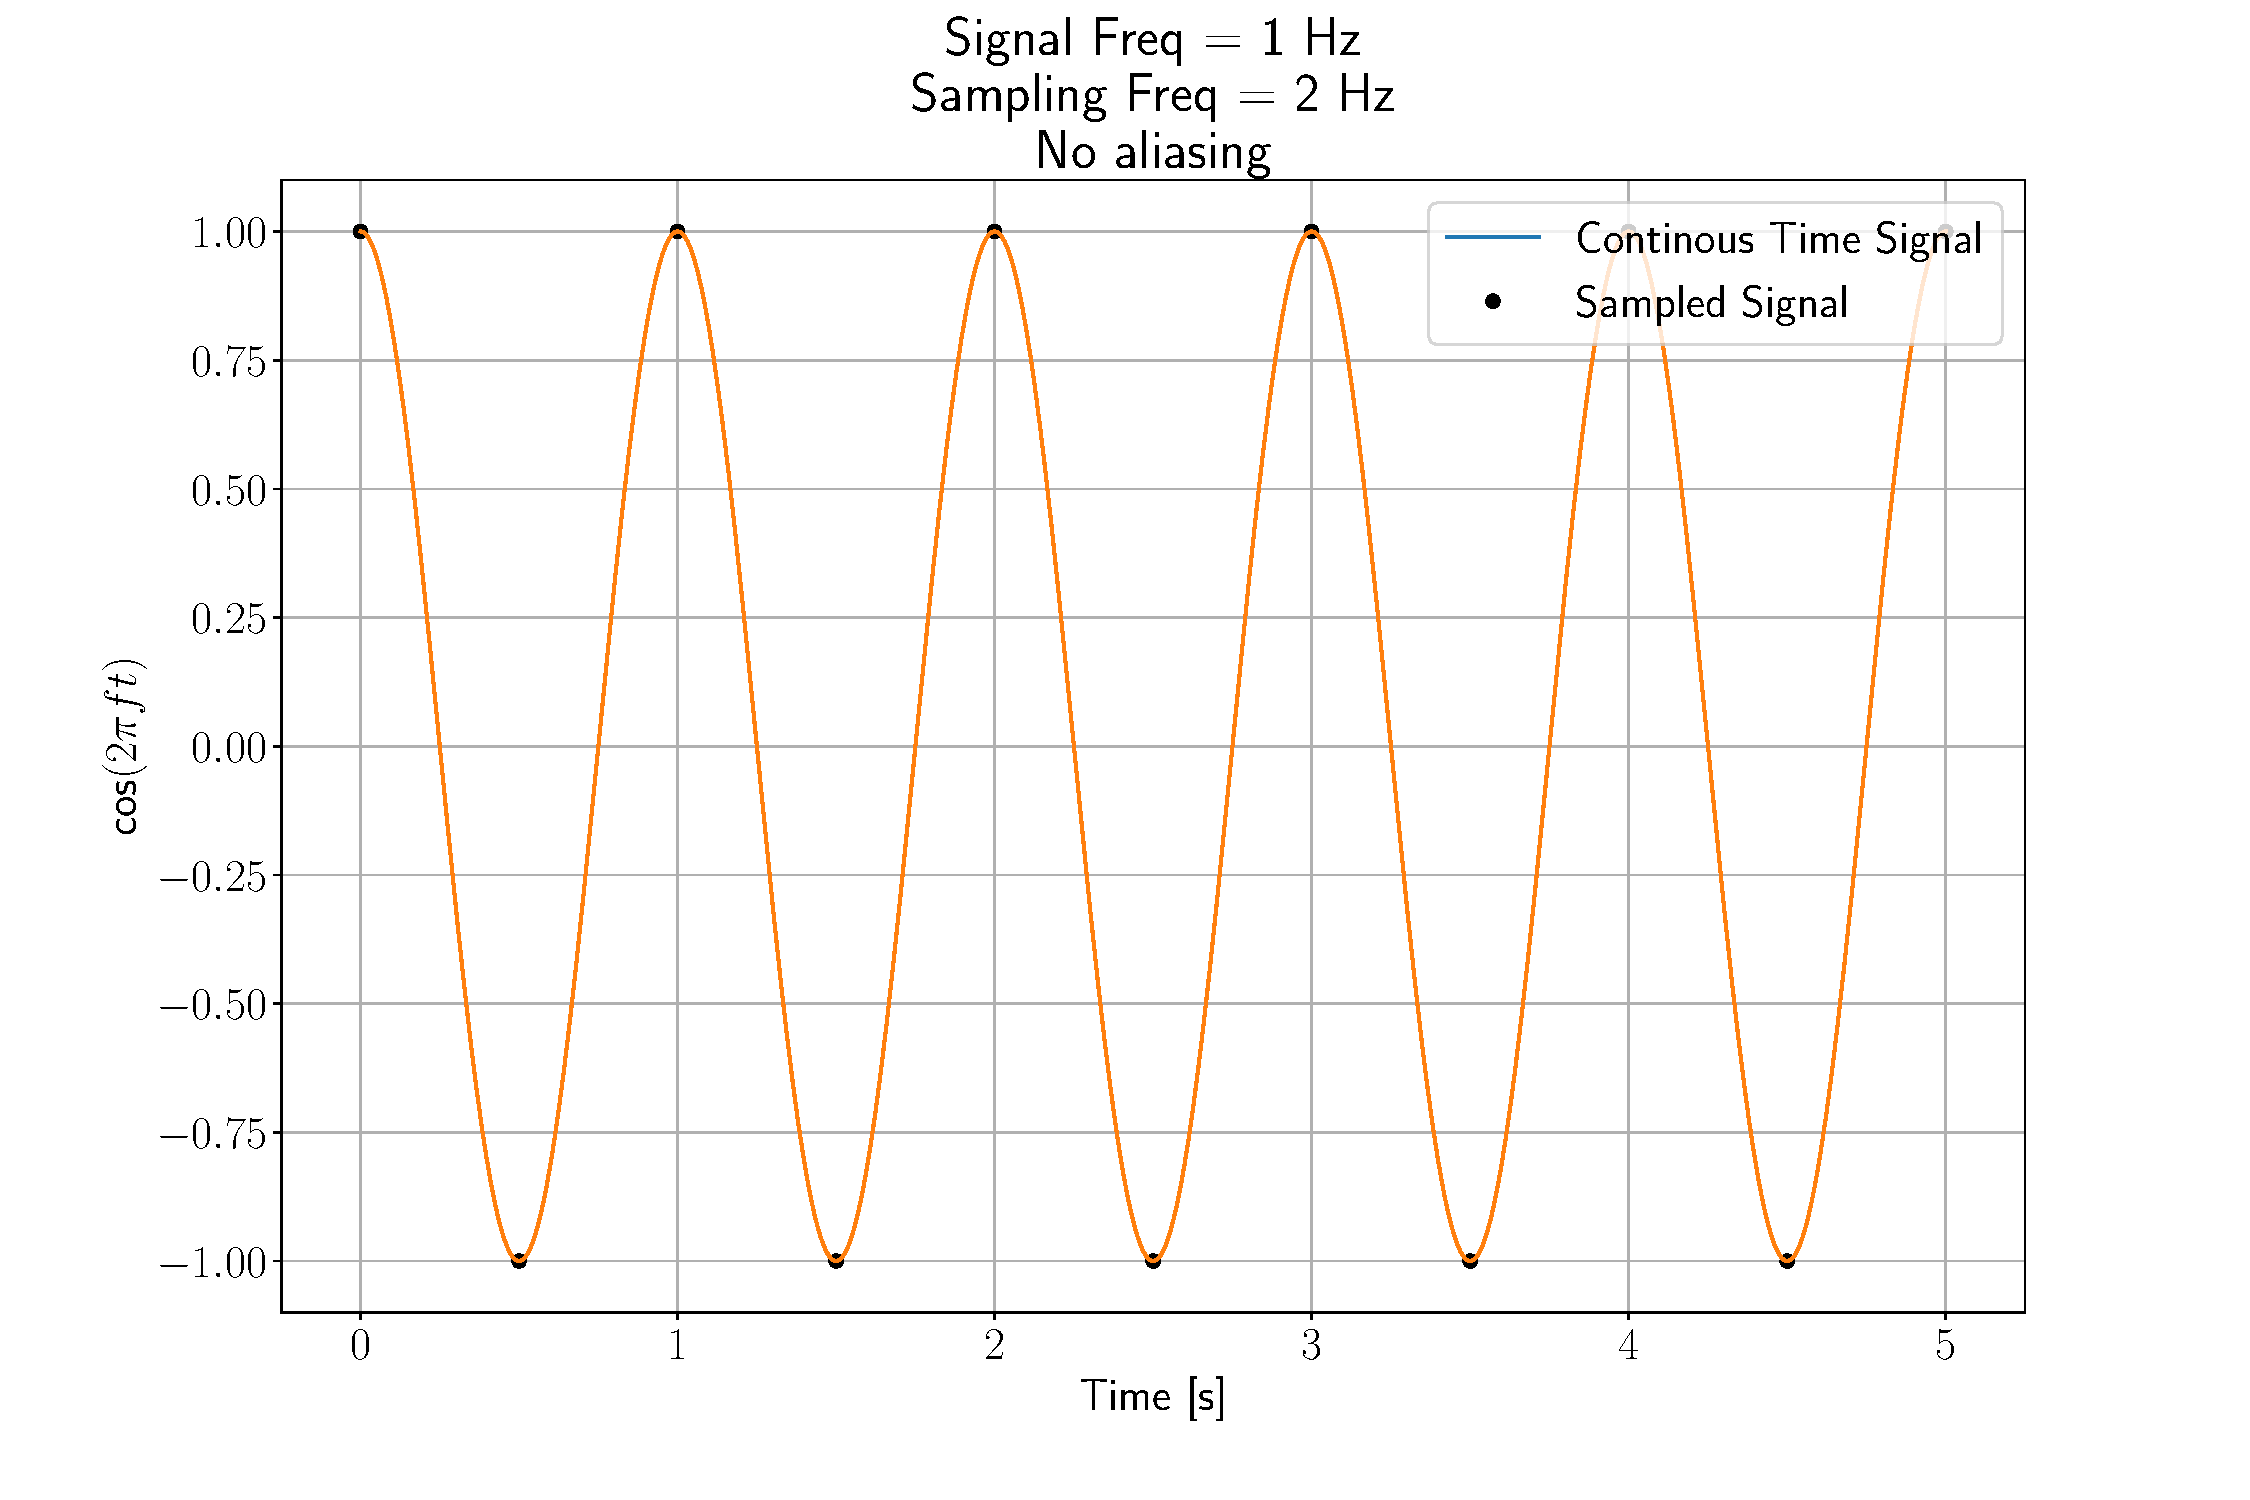
\includegraphics[width = 0.6\textwidth]{Figures/Simulation_Sampling_Frequency_Analysis/Signal_No_Alias_0}
\caption{Sampling at Nyquist Rate: No Aliasing occur}
\label{fig:Simulation_Sampling_Frequency_Analysis:Signal_No_Alias_0}
\end{figure}

\begin{itemize}

\item The signal is from 1 to 5s with a time step of 1ms.

\end{itemize}

\newpage
\begin{figure}[h]
\centering
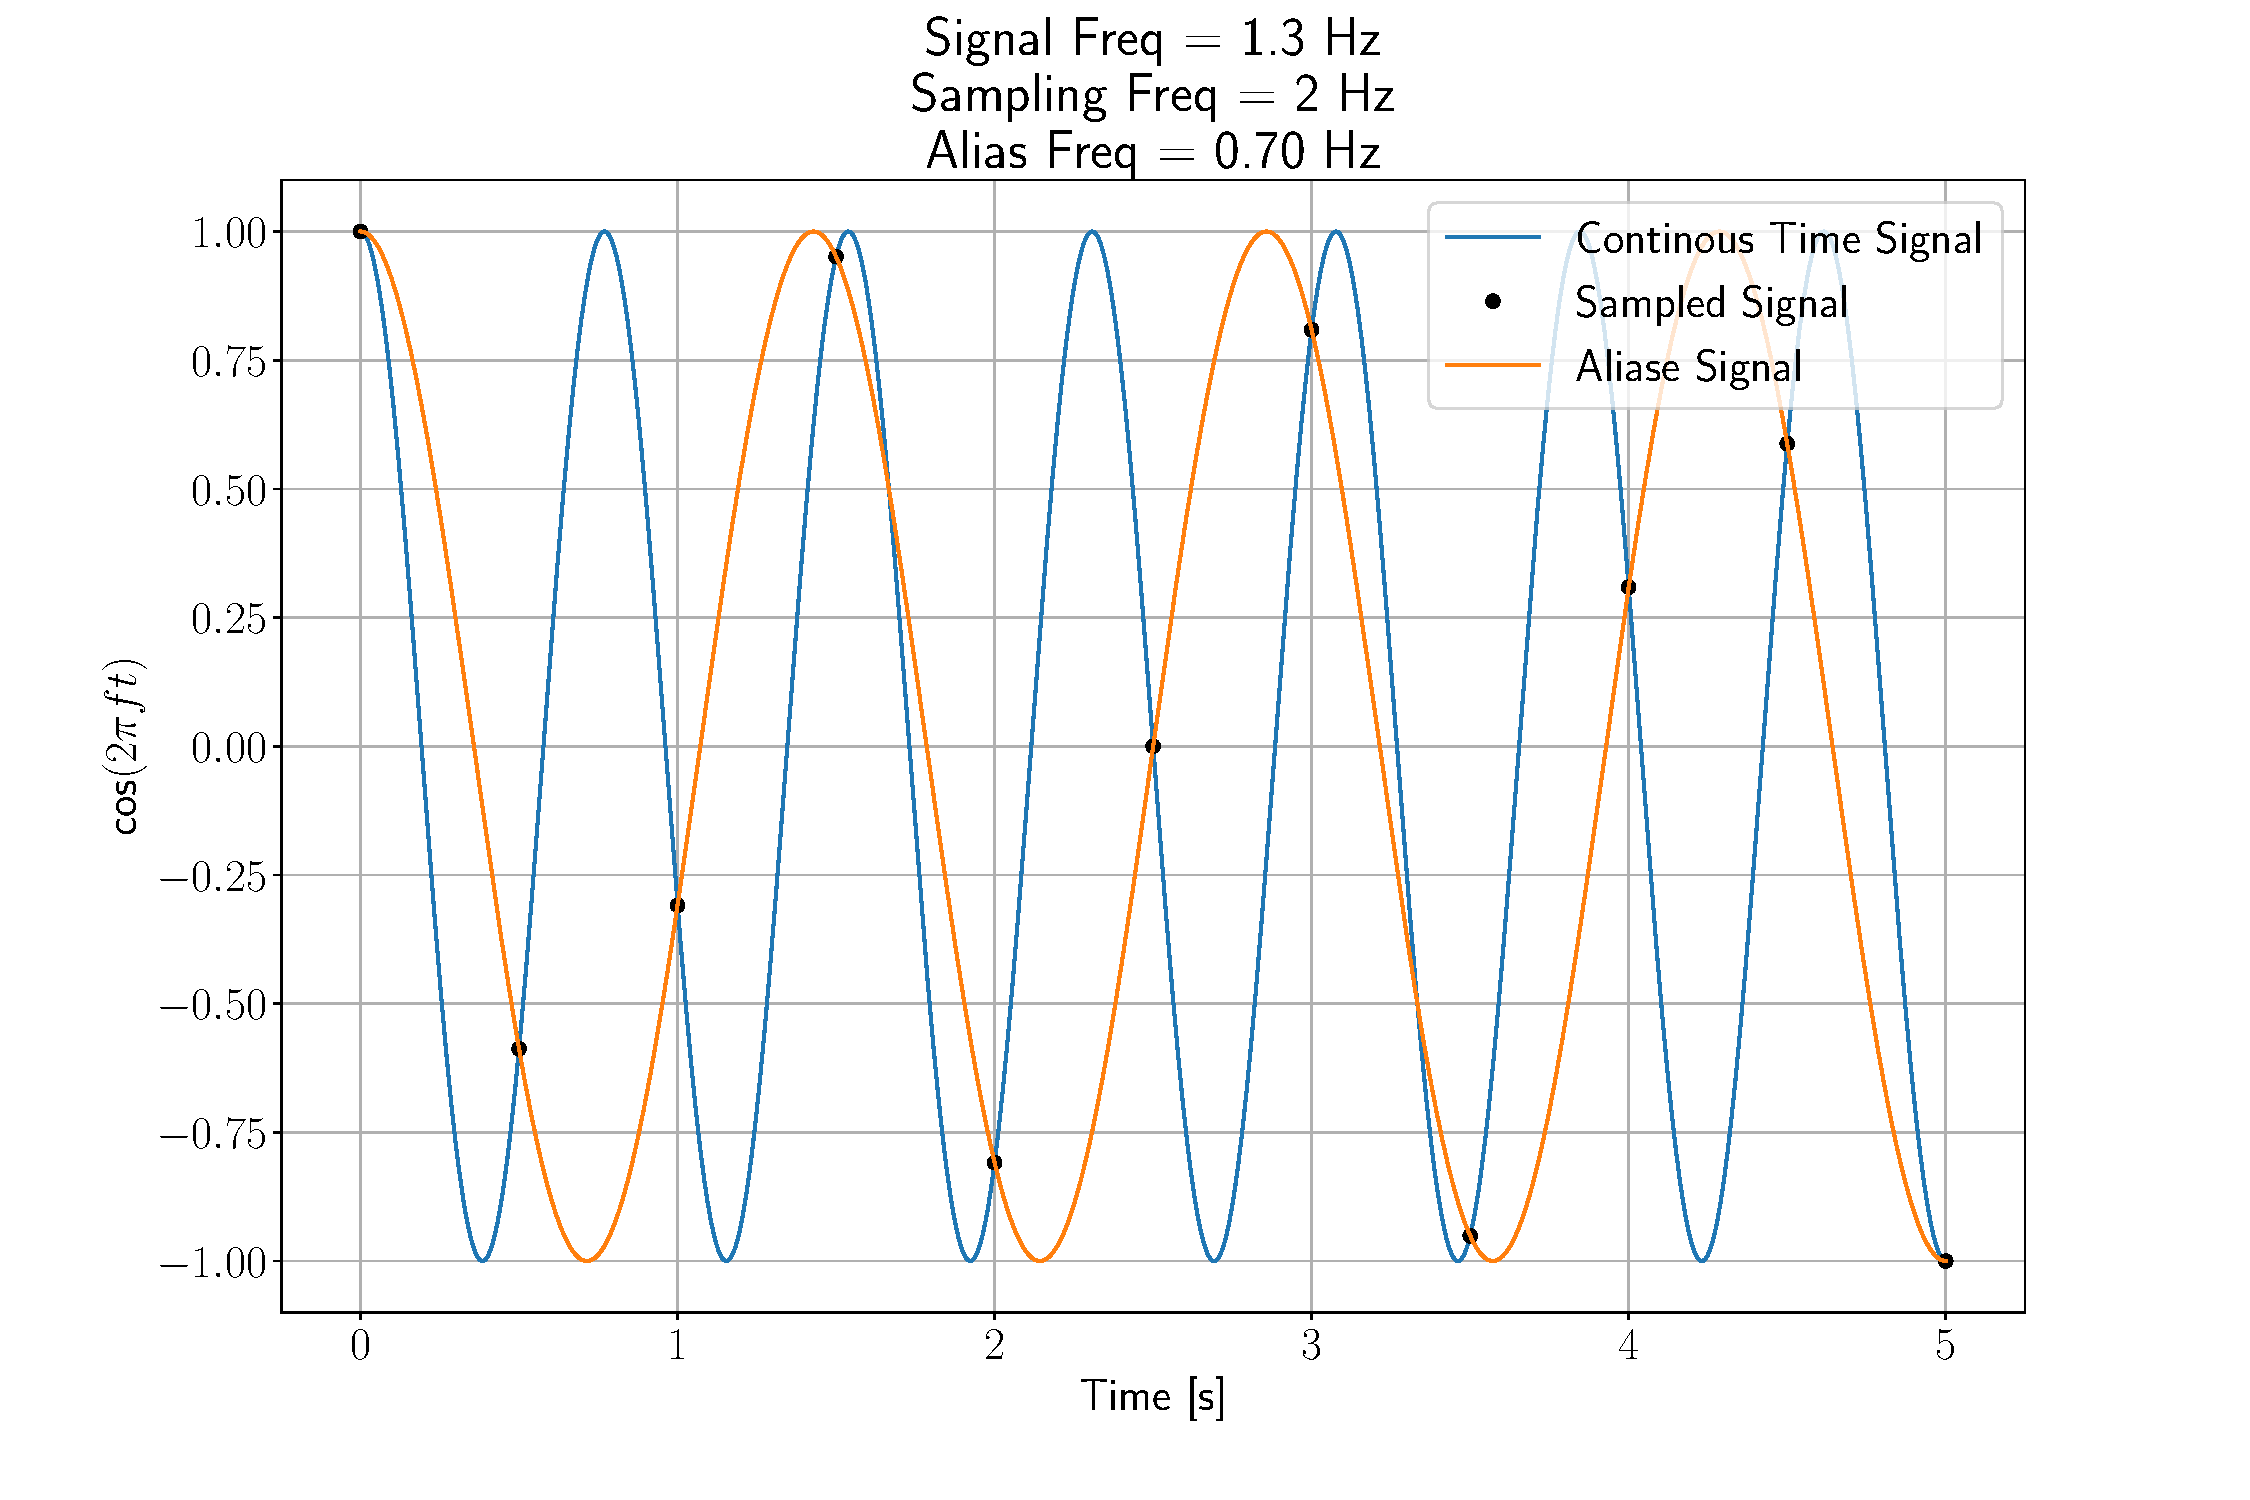
\includegraphics[width = 0.6\textwidth]{Figures/Simulation_Sampling_Frequency_Analysis/Signal_Alias_0_70}
\caption{Increasing Signal Frequency}
\label{fig:Simulation_Sampling_Frequency_Analysis:Signal_Alias_0_70}
\end{figure}

\begin{itemize}

\item Signal frequency is increased and Nyquist rate is not respected now

	\begin{itemize}
	\item $F_s \, < \, 2 \, f_{\text{signal}}$
	\end{itemize}

\item As a result aliasing occur at $f_{\text{alias}} \, = \, 0.7 $ Hz

\end{itemize}


\newpage
\begin{figure}[h]
\centering
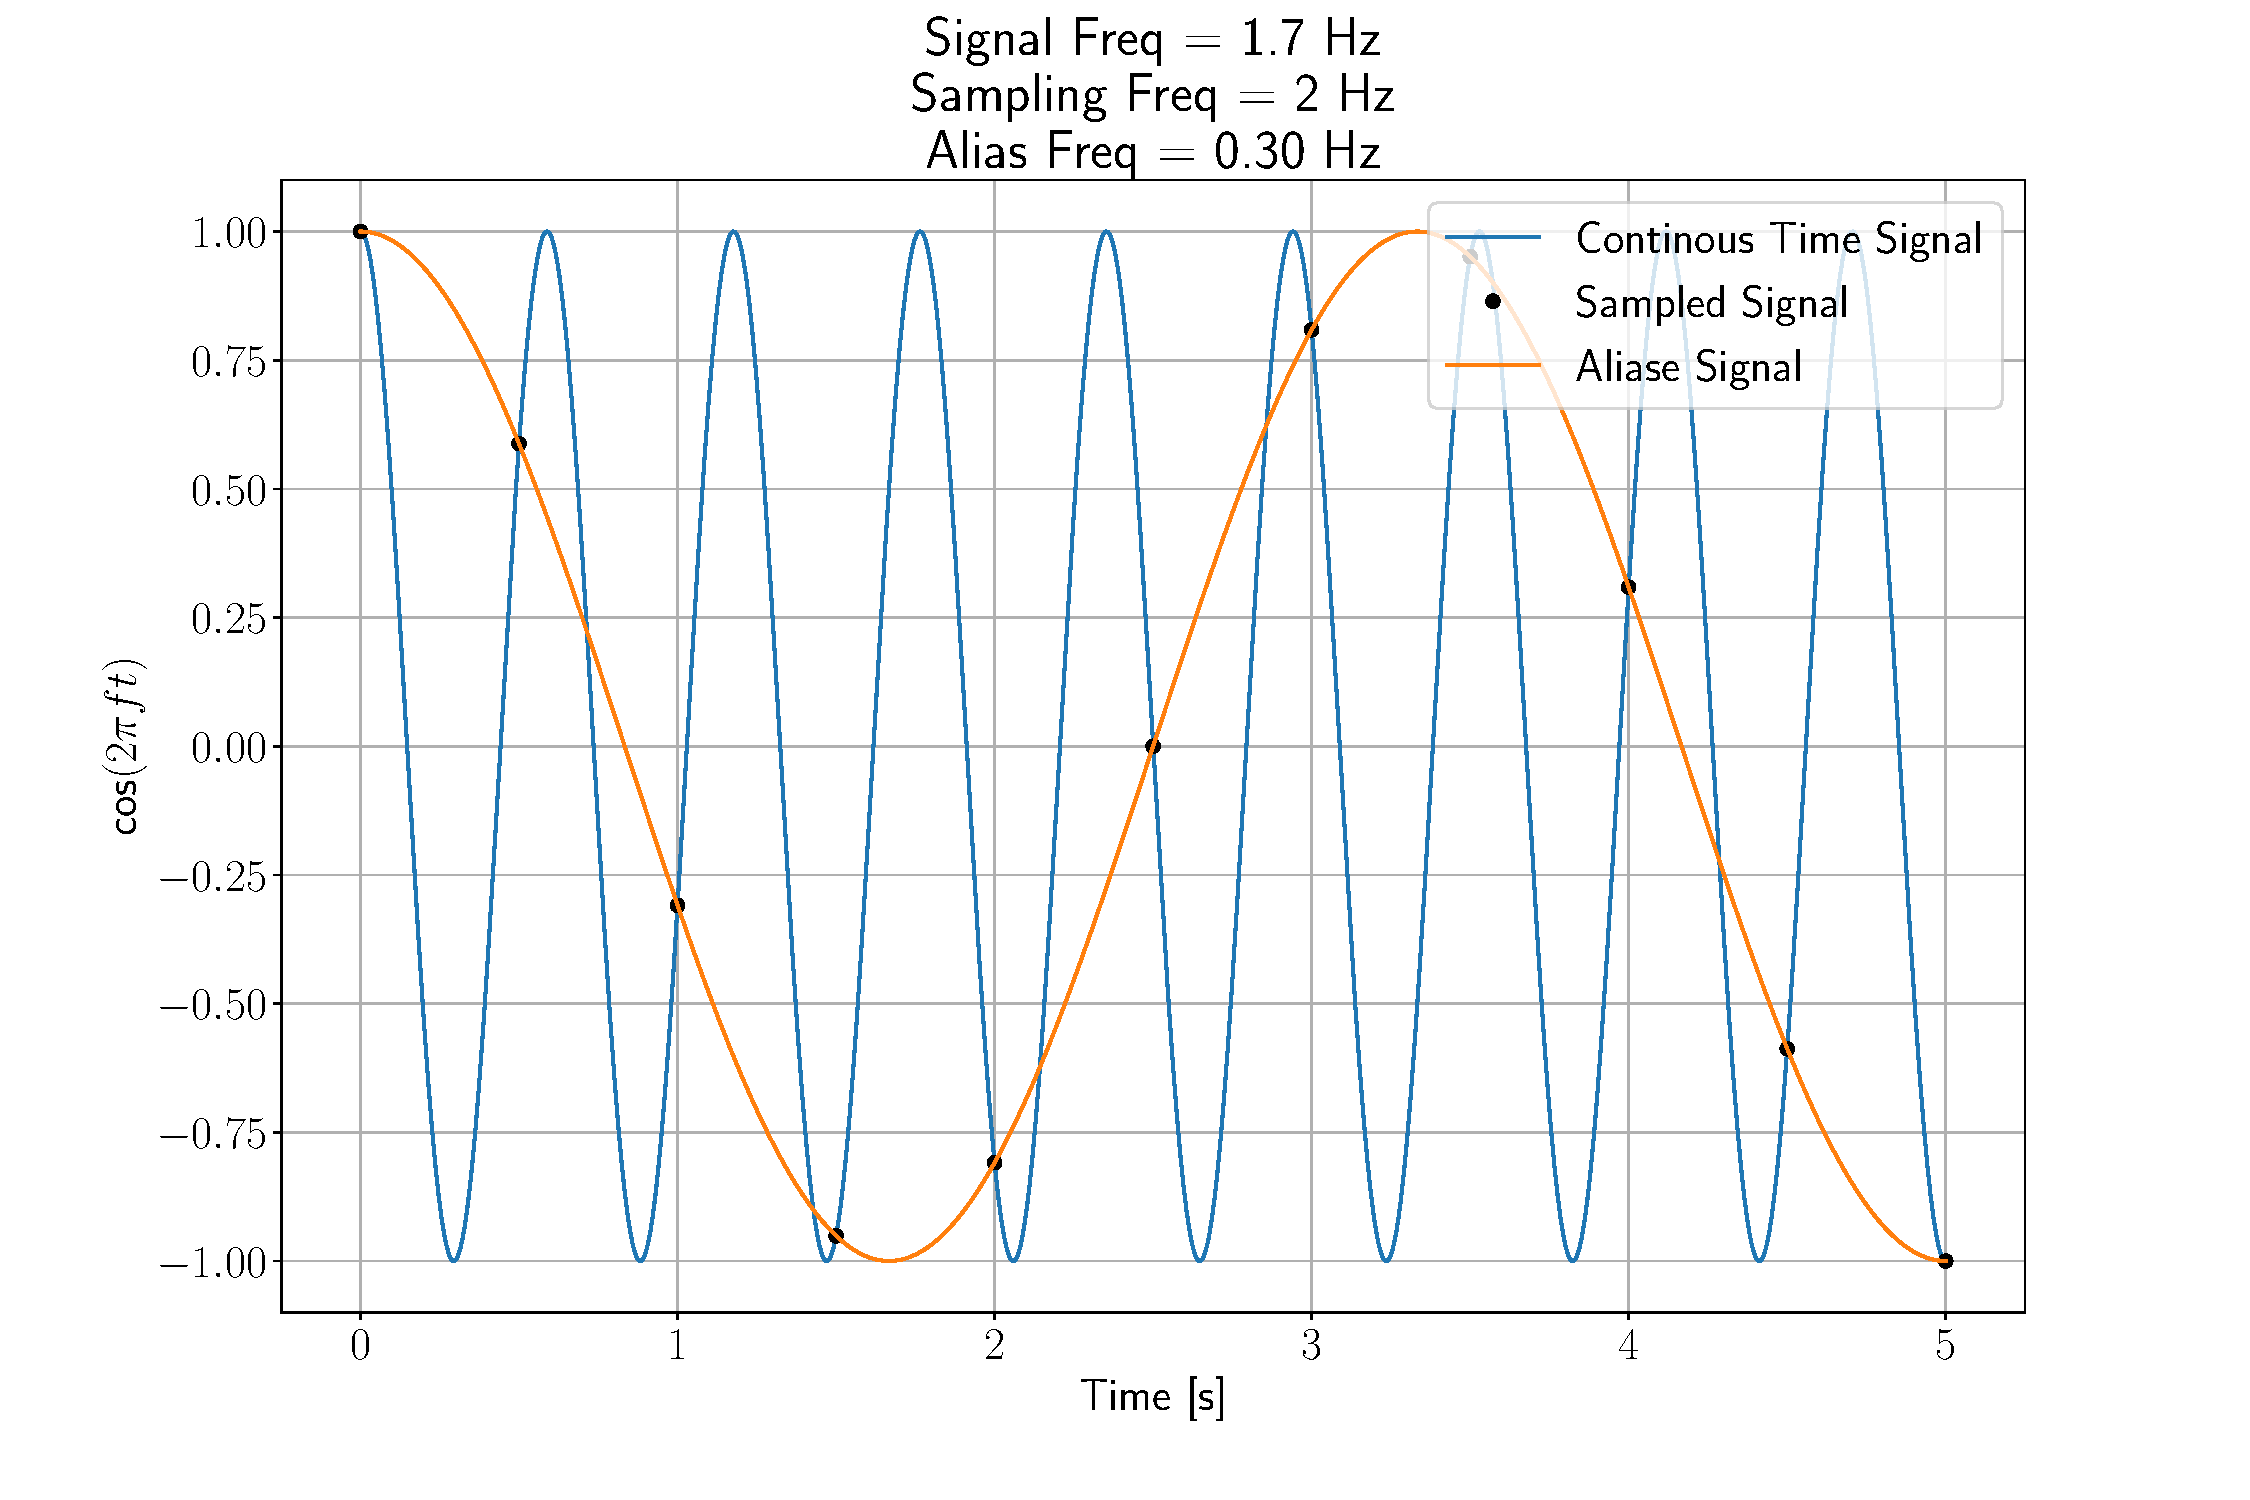
\includegraphics[width = 0.6\textwidth]{Figures/Simulation_Sampling_Frequency_Analysis/Signal_Alias_0_30}
\caption{Sampling at Nyquist Rate: No Aliasing occur}
\label{fig:Simulation_Sampling_Frequency_Analysis:Signal_Alias_0_30}
\end{figure}


\begin{itemize}

\item The signal frequency is even more lower

\item The more we get to the Nyquist rate, the lower $f_{\text{alias}}$ is

	\begin{itemize}
	\item We fail to capture signal information (here frequency content)
	\end{itemize}

\end{itemize}

\end{frame}




\subsection{Zero Padding on FFT for CTFT}
\begin{frame}[t,allowframebreaks]{Zero Padding for the CTFT}

\begin{figure}[h]
\centering
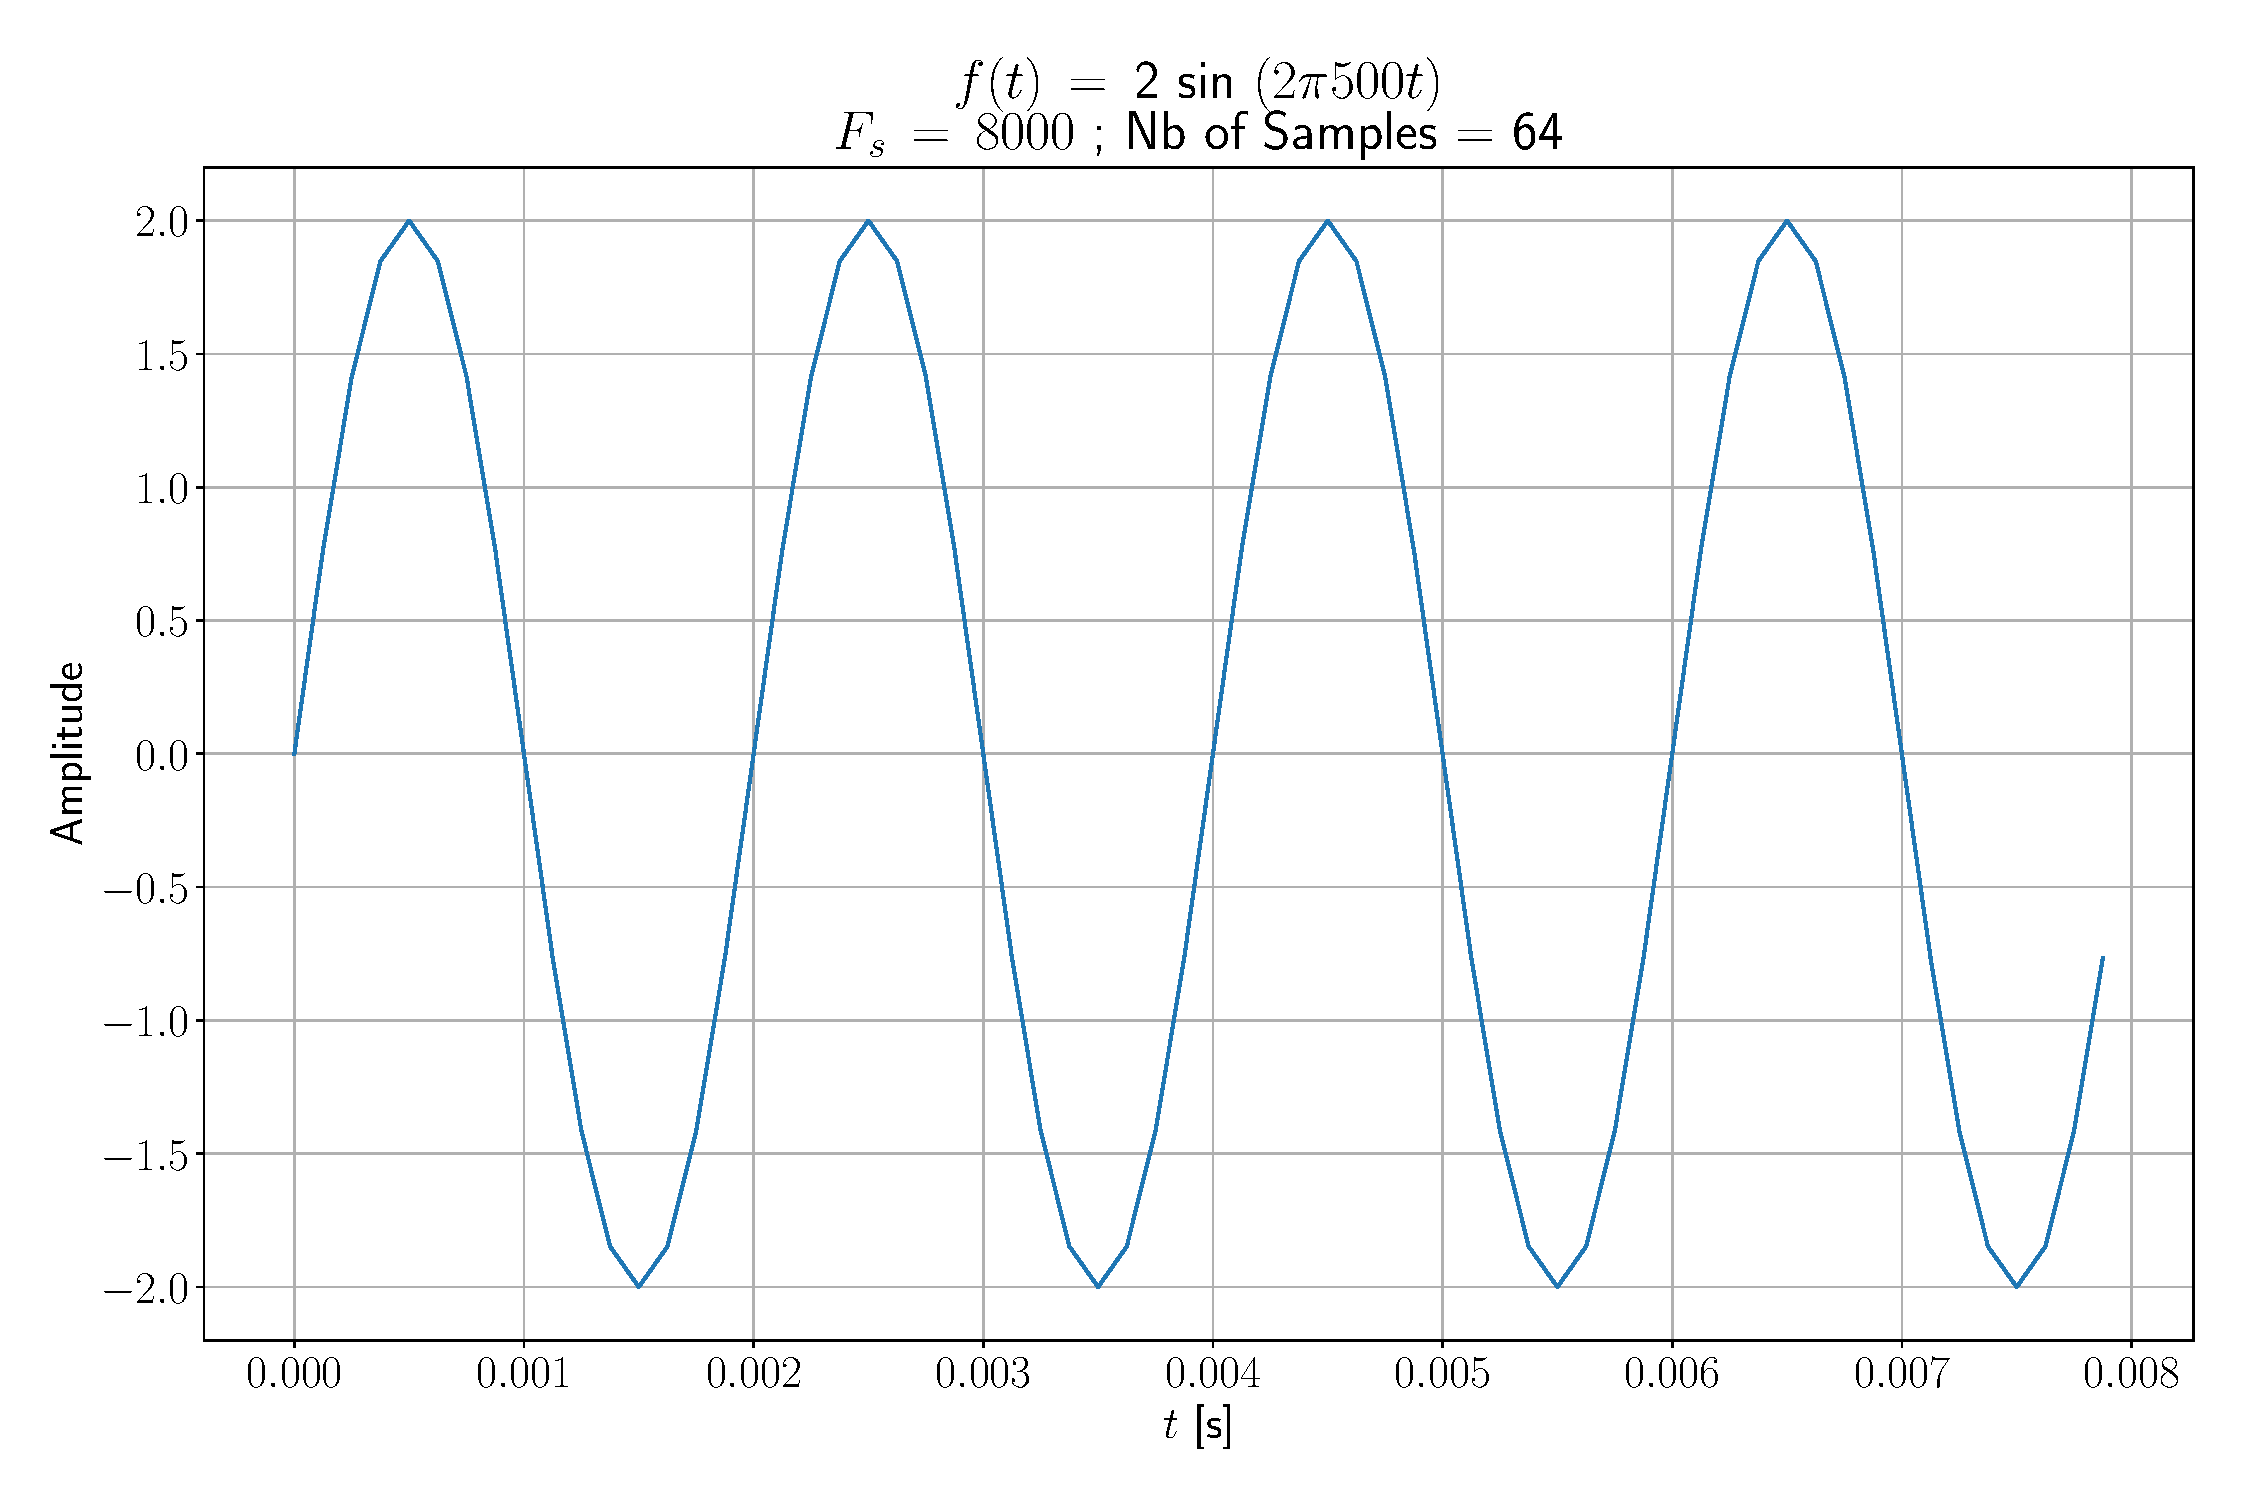
\includegraphics[width = 0.8\textwidth]{Figures/Simulation_Sampling_Frequency_Analysis/Spectral_Analysis_1_Sin_time_domain}
\caption{Time Domain Signal to be worked on}
\label{fig:Simulation_Sampling_Frequency_Analysis:Spectral_Analysis_1_Sin_time_domain}
\end{figure}


\begin{figure}[h]
\centering
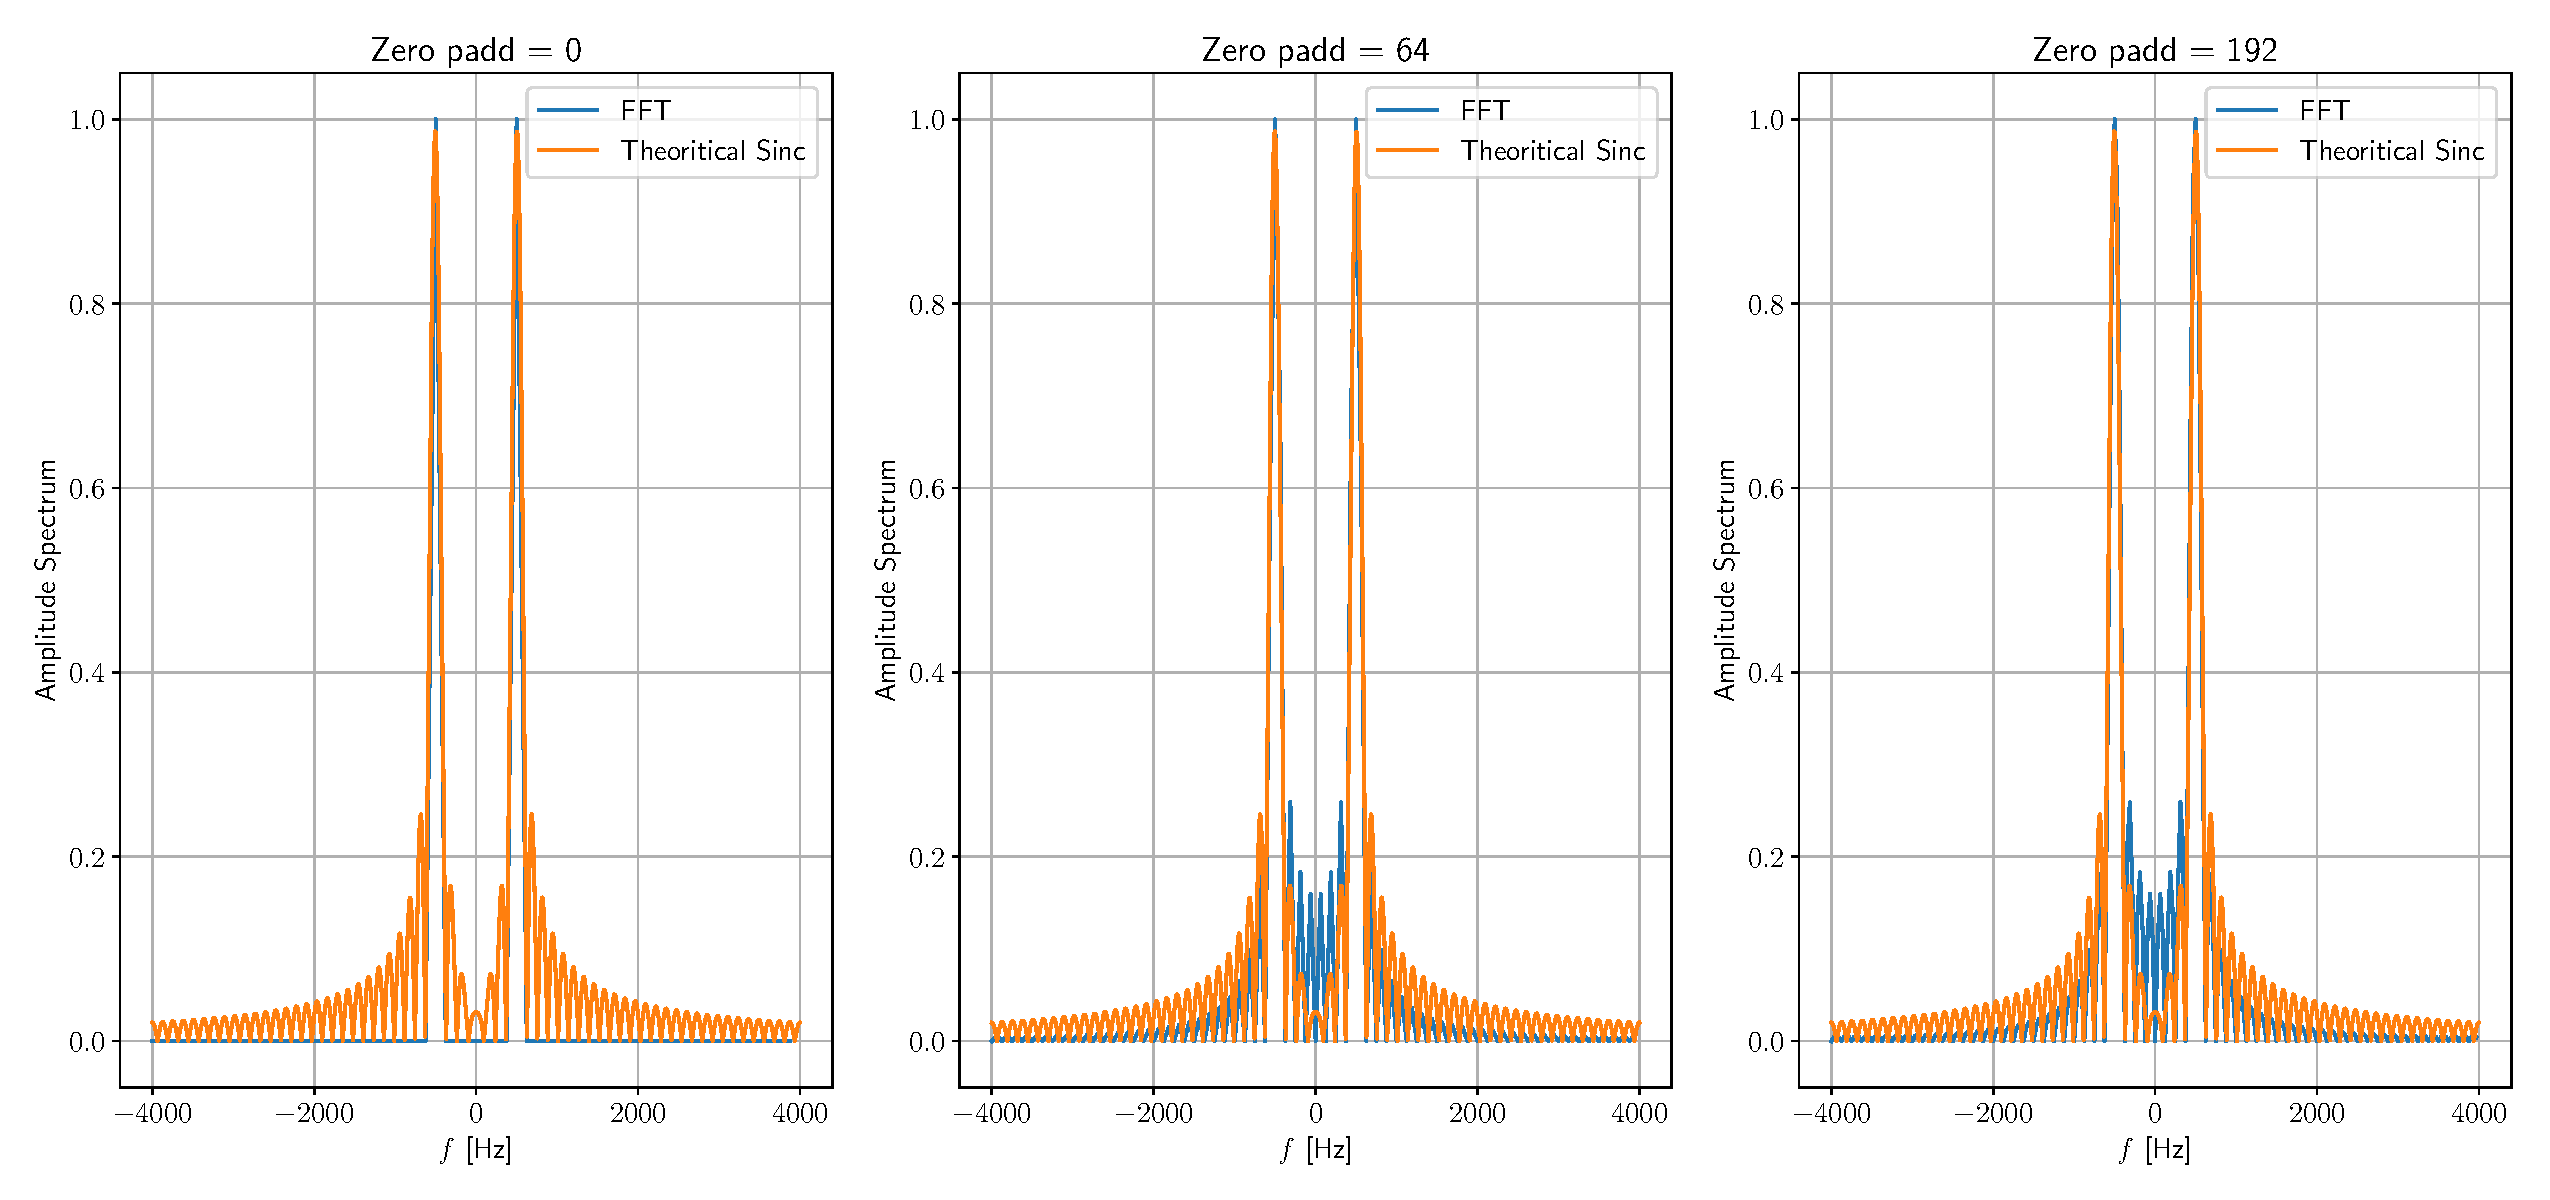
\includegraphics[width = 1\textwidth]{Figures/Simulation_Sampling_Frequency_Analysis/Spectral_Analysis_1_Sin}
\caption{Theoritical and Computed Spectrum using FFT}
\label{fig:Simulation_Sampling_Frequency_Analysis:Spectral_Analysis_1_Sin}
\end{figure}

\newpage

\begin{itemize}

\item If length of the FFT is the same of the length of the signal, no zero padding occur

\item If length of the FFT $>$ bigger then length of the signal, the signal will be padded with 0

	\begin{itemize}
	\item More \textcolor{red}{dense spectrum} is obtained $\leftrightarrow$ better displayed version $\leftrightarrow$ longer DFT sequence
	\end{itemize}

\end{itemize}


\end{frame}




%**************************************************
%**************************************************
%**************************************************

\section{Multirate Signal Processing}
\label{Chap:Multirate}
\begin{frame}[t]{Chapter \autoref{Chap:Multirate}}
\tableofcontents[sections= \value{section}]
\end{frame}


\subsection{Introduction and Motivation}
\begin{frame}[t,allowframebreaks]{Introduction to Multirate Signal Processing}

\begin{itemize}

\item Multirate Signal processing: the field of signal processing which have \textcolor{red}{several sampling rate exist in the system} \cite{DSP_DimitrisManolakis}

\item The changing in sampling rate occurs much often in real world systems

    \begin{itemize}
        \item For example, we have a system A expect data at a sampling rate 10 KHz
        
        \item Another system B expect data at a sampling rate 12 KHz
        
        \item How can I make the 2 systems talk to each other?
        
    \end{itemize}

\end{itemize}


\end{frame}



\subsection{Reminder: Sampling and Notation}
\begin{frame}[t,allowframebreaks]{Reminder about Original Sampling and Notation}


\begin{figure}[h]
\centering
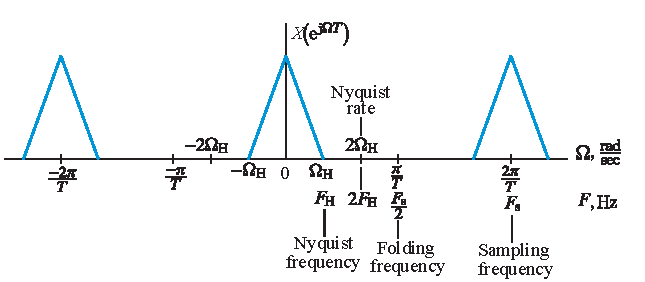
\includegraphics[scale=0.9]{Figures/Sampling/Impulse_Sampling_Terminology}
\caption{Replicated Amplitude Spectrum: Frequency axis in $F$[Hz] and $\omega_c$[rad/s] \cite{DSP_DimitrisManolakis}}
\label{fig:Sampling:Impulse_Sampling_Terminology}
\end{figure}

\begin{itemize}

\item Recall that when sampling in time, images are created at multiple of $F_s$ in CTFT domain along with a scaling factor $\displaystyle\frac{1}{T_s}$


\item This effect will be compared to the effect done by downsampling and upsampling operation to our spectrum

	\begin{itemize}
	\item In other words, we will compare the spectrum after doing down(up)sampling to the spectrum of $X_\delta(\omega_c)$
	\end{itemize}

\item \underline{Notation:} Because now we have some new sampling rate as we will see later, we adopt the following notation for the sampling rate:

	\begin{itemize}
	\item When doing normal Nyquiste sampling $\leftrightarrow \, T_{s_{\text{original}}}$
	
	\item Downsampling $ \leftrightarrow \, T_{\text{downsample}}$
	
	\item Upsampling $ \leftrightarrow \, T_{\text{upsample}}$
	\end{itemize}

\end{itemize}

\end{frame}


\subsection{Downsampling}
\begin{frame}[t,allowframebreaks]{Downsampling Operation}

\begin{figure}[h]
\centering
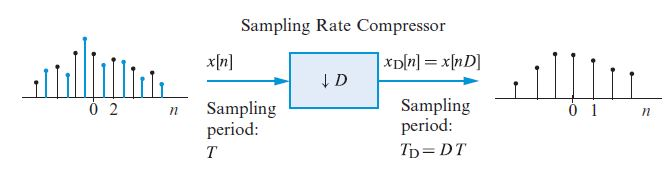
\includegraphics[width = 0.7\textwidth]{Figures/Multirate/dowsampling_block_diagram}
\caption{Block diagram representation of sampling rate compressor system \cite{DSP_DimitrisManolakis}}
\label{fig:Multirate:dowsampling_block_diagram}
\end{figure}

\begin{itemize} 

\item Dowsampling: throwing away samples

\item Vocabulary: downsampler = sampling rate compressor

\item The operation is \textcolor{red} {in the discrete time domain} $x[k]$

\item What happens when we do dowsampling?

	\begin{itemize}
	\item The answer is in the amplitude spectrum 
	\end{itemize}


\end{itemize}
\end{frame}



\begin{frame}[t,allowframebreaks]{Dowsampling Effect on CTFT Amplitude Spectrum}

\begin{itemize}
\item First let's examine relation in the \textcolor{red}{continuous time frequency spectrum}

	\begin{itemize}
	\item Math governing \cite{DSP_DimitrisManolakis}
	
	\end{itemize}

	\begin{equation}
	\begin{array}{rcl}
		X_{\text{decimated}}(\omega_c) \, &=& \, \displaystyle	\frac{1}{T_{\text{downsample}}} \, \displaystyle\sum_{i \, = \, -\infty}^{\infty} X \left(\,  \omega_c \, - \, i \, \omega_{\text{downsample}} \,\right) \\ \\
		&=& \, \displaystyle\frac{1}{T_{s_{\text{original}}} \, D} \, \displaystyle\sum_{i \, = \, -\infty}^{\infty} X \left(\, \omega_c \, - \, \displaystyle\frac{2 \pi}{T_s \, D} \, i \,\right)
\end{array}
\label{Eq:Multirate:Decimation_spectrum_ctft}	
	\end{equation}		

where $\begin{cases}
T_{\text{downsample}} \, = \, D \, \times \, T_{s_{\text{original}}}\\
\omega_{\text{downsample}} \, = \, \displaystyle\frac{2 \pi}{D} \, = \,\displaystyle\frac{\omega_{s_{\text{original}}}}{D} \\
D \, \in \mathbb{N}
\end{cases}$

\begin{figure}[h]
\centering
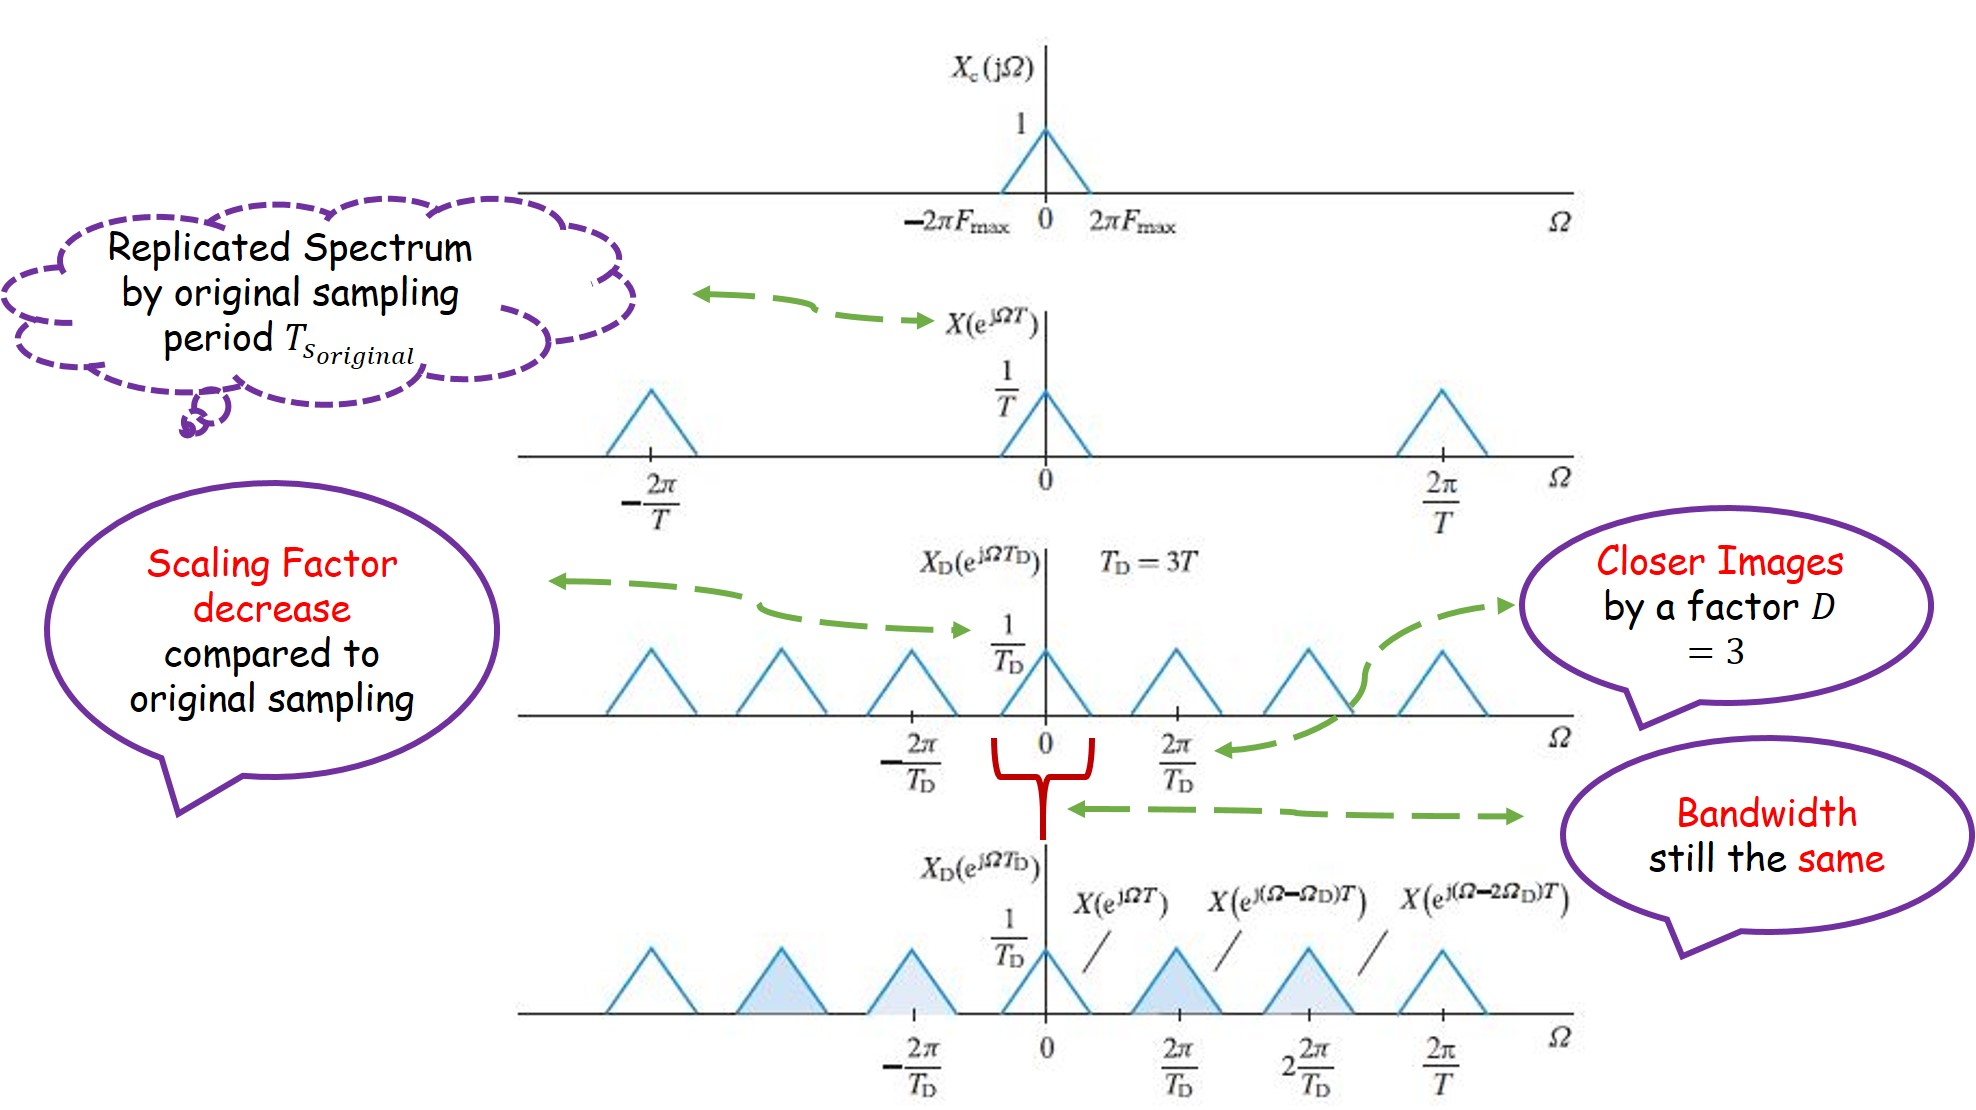
\includegraphics[width = 0.7\textwidth]{Figures/Multirate/dowsampling_ctft_summary}
\caption{Graphical Illustration for equation (\autoref{Eq:Multirate:Decimation_spectrum_ctft}) for CTFT spectrum \cite{DSP_DimitrisManolakis}}
\label{fig:Multirate:dowsampling_ctft}
\end{figure}


\newpage
\item Also keep in mind that we could avoid aliasing by respecting the Nyquiste rate for downsampling

	\begin{itemize}
	\item $\omega_{\text{downsample}} \, = \, \displaystyle\frac{2 \pi}{T_{\text{downsample}}} \, > \, 2 \, \omega_{\text{max}}$
	\end{itemize}

\end{itemize}

\end{frame}



\begin{frame}[t,allowframebreaks]{Dowsampling Effect on DTFT Amplitude Spectrum}

\begin{itemize}
\item Relation between $X_{\text{DTFT}}(\omega_d) $ and $X_{\text{decimated}}(\omega_d) $ 
	
	
	\begin{equation}
	\begin{array}{rcl}
		X_{\text{decimated}}(\omega_d) \, = \, \displaystyle	\frac{1}{D} \, \displaystyle\sum_{i \, = \, 0}^{D \, - \, 1} X_{\text{DTFT}} \left(\,  \displaystyle\frac{\omega_d}{D} \, - \, \displaystyle\frac{2 \pi}{D} \, i \,\right)   
	\end{array}	\label{Eq:Multirate_Sampling_Decimation_spectrum_dtft_relation}
	\end{equation}		
	
	\begin{itemize}
			
	\item A \textcolor{red}{Surprise!}: equation (\ref{Eq:Multirate_Sampling_Decimation_spectrum_dtft_relation}) tells us that our \textcolor{red}{bandwidth will expand (stretch)} by a factor of $D$.

	\end{itemize}


\newpage
\item Some graphical illustrations:


\begin{figure}[h]
\centering
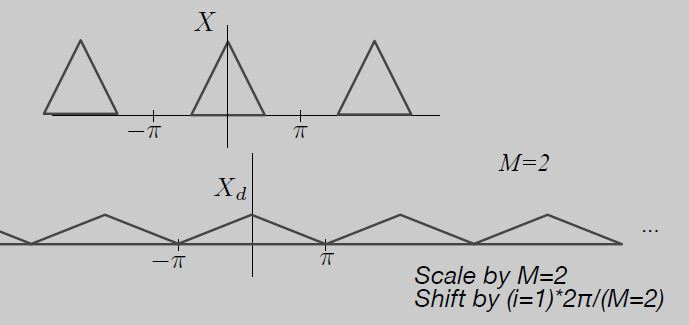
\includegraphics[width = 0.7\textwidth]{Figures/Multirate/dowsampling_example_m_2}
\caption{Downsampling by a factor $D \, = \, 2$}
\label{fig:Multirate:dowsampling_example_m_2}
\end{figure}


	\begin{itemize}
	\item Stretching in the bandwidth
	
	\item Dowsampling $\rightarrow F_s$ decrease $\rightarrow$ replicate will be more closer together
	
	\end{itemize}

\end{itemize}
\end{frame}


\begin{frame}[t,allowframebreaks]{More Dowsampling}



\begin{itemize}


\item Let's downsample more: \textcolor{red}{aliasing occurs !}
	
\begin{figure}[h]
\centering
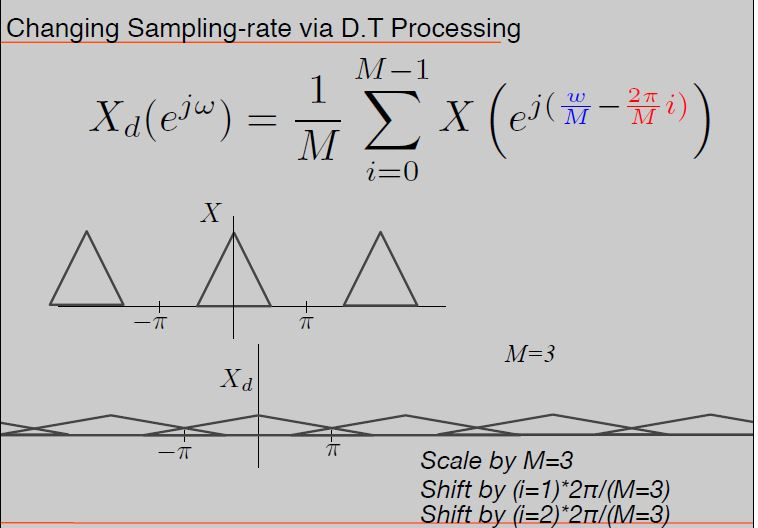
\includegraphics[width = 0.7\textwidth]{Figures/Multirate/dowsampling_example_m_3}
\caption{Downsampling by a factor $M \, = \, 3$ Aliasing occur}
\label{fig:Multirate:dowsampling_example_m_3}
\end{figure}

\newpage
	\item Solution: put an anti-alias filter but in the discrete domain
	
\begin{figure}[h]
\centering
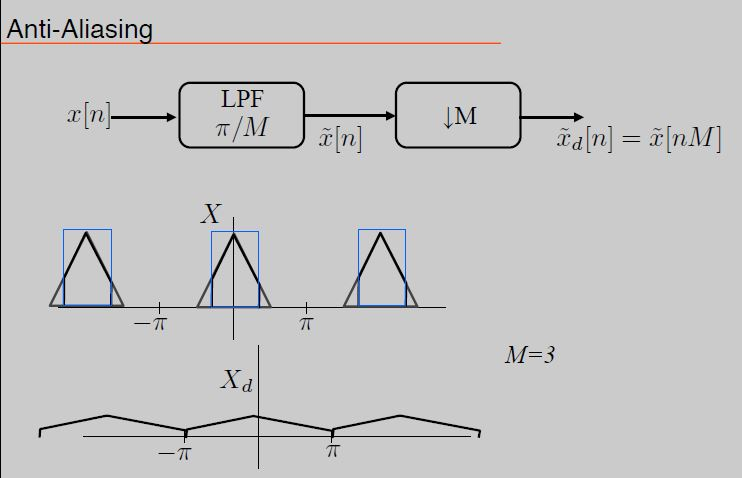
\includegraphics[width = 0.6\textwidth]{Figures/Multirate/dowsampling_antialias_filter}
\caption{Antialias filter then dowsample because downsample can't afford to represent high frequency components}
\label{fig:Multirate:dowsampling_example_m_3}
\end{figure}	
	
		\begin{itemize}
		\item Anti-imaging design choice: $\omega_{\text{cut-off}} \, = \, \displaystyle\frac{\pi}{D}$
		\end{itemize}



\end{itemize}

\end{frame}


\subsection{Upsampling}
\begin{frame}[t,allowframebreaks]{Upsampling Introduction}

\begin{itemize}

\item Very much like to digital-to-analog converter

	\begin{itemize}
	\item Not the same, but they have similarities
	\end{itemize}

\item Recall our ideal digital-to-analog process:

	\begin{itemize}
	\item $x[n] \, = \, x_{\delta}(t) \, \rightarrow \, x_{\text{interpolated}}(t)$, where we have done interpolation using a sinc
	\end{itemize}

\end{itemize}

\end{frame}


\begin{frame}[t,allowframebreaks]{Upsamling Implementation}


\begin{itemize}


\item To implement upsampling, we will do the same thing as in DAC \textcolor{red}{but in the discrete domain}

	\begin{enumerate}	

	\item Start from $x[n]$
	
	\item Expanding by placing 0 between adjacent samples, this will give us $x_{\text{expanded}}[n]$

	\begin{equation}
	x_{\text{expanded}}[n] \, = \, \begin{cases}
	x\left[\, \displaystyle\frac{n}{L} \,\right] \quad n \, =\, 0 \, ; \, \pm L \, ; \, \pm 2L \, \cdots \\
	0 \quad \text{otherwise}
	\end{cases}
	\label{Eq:Multirate:Exapanding}
\end{equation}		

\begin{figure}[h]
\centering
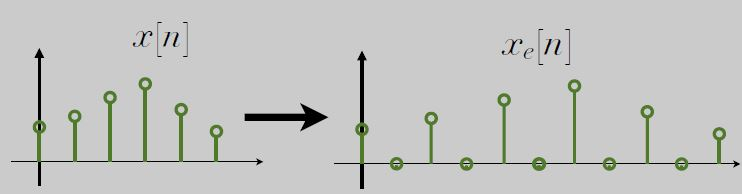
\includegraphics[width = 0.6\textwidth]{Figures/Multirate/upsampling_expansion}
\caption{Expansion in the discrete time domain}
\label{fig:Multirate:upsampling_expansion}
\end{figure}
	
	\begin{itemize}
	\item The expansion of equation (\ref{Eq:Multirate:Exapanding}) also can be viewed as a convolution between the orignal discrete time signal $x[n]$ and a \textcolor{red}{shifted discrete delta}
	
	\begin{equation}
	x_{\text{expanded}}[n] \, = \, \displaystyle\sum\limits_{i \, = \, - \infty}^{\infty} x[i] \, \times \,  \delta[n \, - \,  i \, L]
\end{equation}		
	
\end{itemize}		
	
	\item Interpolation of the expanded signal using a \textcolor{red}{discrete time} sinc 
	
		\begin{itemize}
		\item Be aware that this is a \textcolor{red}{bandlimited interpolation}
		\end{itemize}
	
\begin{figure}[h]
\centering
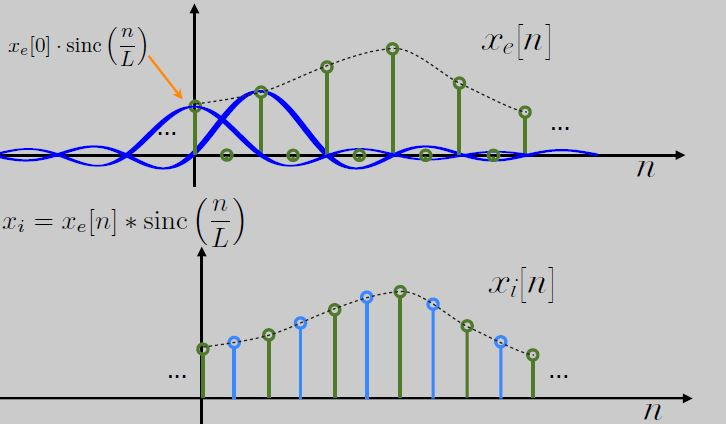
\includegraphics[width = 0.6\textwidth]{Figures/Multirate/upsampling_convolution}
\caption{Convolving the expanded signal with discrete time sinc (bandlimited interpolation)}
\label{fig:Multirate:upsampling_convolution}
\end{figure}


	
 \end{enumerate}

 
\end{itemize}

\end{frame}


\begin{frame}[t,allowframebreaks]{Upsampling Effect on DTFT spectrum}

\begin{itemize}

\item Upsampling \textcolor{red}{compress the DTFT spectrum} by a factor of $L$ \textcolor{cyan}{and} \textcolor{red}{ create replications (Images) also}

\begin{itemize}

\item This is expected since upsampling is like resampling , and we already know that sampling creates images of a spectrum
\end{itemize}

\item \underline{Proof:}

\begin{enumerate}

\item Begin with DTFT definition for the expanded signal $x_{\text{expanded}}[k]$

\begin{equation}
X_{\text{expanded}}(\omega_d)  =  \displaystyle\sum\limits_{k \, = \, - \infty}^{+\infty} x_{\text{expanded}}[k] \, e^{-j \, \omega_d \, k} 
\end{equation}


\item However, we note from equation (\autoref{Eq:Multirate:Exapanding}) that $x_{\text{expanded}}[k]$ exist only for multiple of $L$, the upsampling factor which means that we can change the limit of summation and sum up only for $k \, = \, m \, L$

\begin{equation}
X_{\text{expanded}}(\omega_d)  =  \displaystyle\sum\limits_{m \, = \, - \infty}^{+\infty} x_{\text{expanded}}[m \, L] \, e^{-j \, \omega_d \, m \,L} 
\end{equation}

\item Note that $x_{\text{expanded}}[m \, L]$ is nothing but $x_{\text{original}}[m]$ at index $m$

\begin{equation}
\begin{array}{rcl}
X_{\text{expanded}}(\omega_d)  &=&  \displaystyle\sum\limits_{m \, = \, - \infty}^{+\infty} x_{\text{original}}[m]\, e^{-j \, \omega_d \, m \,L}  \\ \\
X_{\text{expanded}}(\omega_d) \, &=& \, X_{\text{original}}(\omega_d \, L)
\end{array}
\end{equation}


\end{enumerate}

\underline{Conclusion:} DTFT spectrum will be compressed 



\item We need to low pass filtering to obtain the desired spectrum


\begin{figure}[h]
\centering
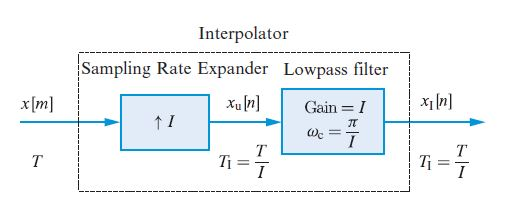
\includegraphics[width = 0.6\textwidth]{Figures/Multirate/interpolation_process}
\caption{Interpolation process: upsampling then low pass filtering \cite{DSP_DimitrisManolakis}}
\label{fig:Multirate:interpolation_process}
\end{figure}


\end{itemize}

\end{frame}

\begin{frame}[t]{Interpolation and Upsampling Recap}


\begin{figure}[h]
\centering
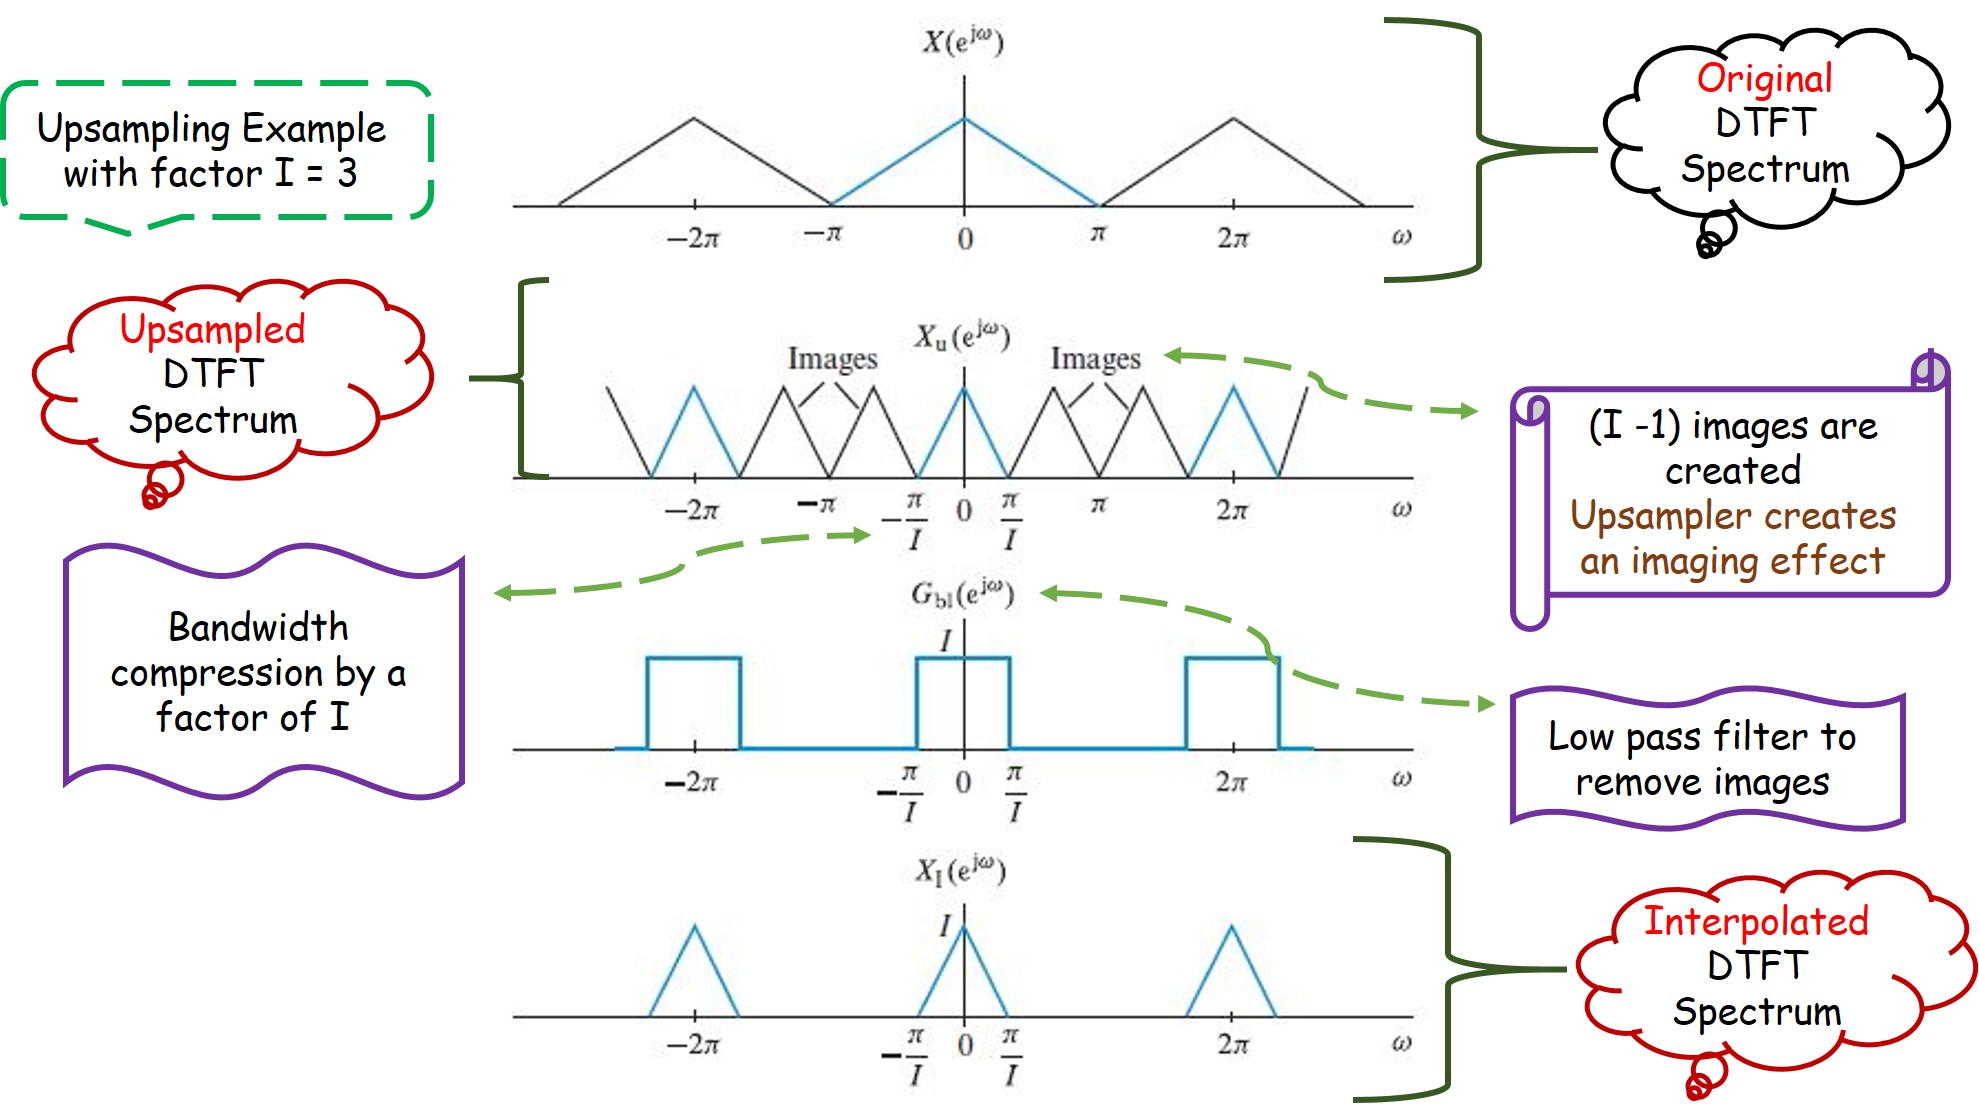
\includegraphics[width = 0.95\textwidth]{Figures/Multirate/upsampling_process}
\caption{Upsampling with a factor $I \, = \, 3$ \cite{DSP_DimitrisManolakis}}
\label{fig:Multirate:interpolation_process}
\end{figure}


\end{frame}


\subsection{Practical Upsampling}
\begin{frame}[t,allowframebreaks]{Practical Upsampling}


\end{frame}

\subsection{Resampling by non-integer factor}
\begin{frame}[t,allowframebreaks]{Resampling by non-integer factor}

\begin{itemize}

\item Sampling rate by a non-integer factor which can be expressed in the form of $T_{s_{\text{new}}} \, = \, T_{s_{\text{original}}} \, \times \, \displaystyle\frac{I}{D}$

\item Example: resample by a factor of $1.5 \, T_{s_{\text{original}}} \, = \, \displaystyle\frac{3}{2} \, T_{s_{\text{original}}}$

\item Idea: use upsampling and dowsampling together

\begin{figure}[h]
\centering
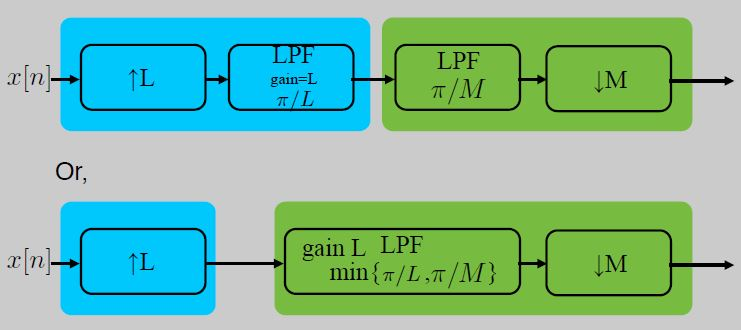
\includegraphics[width = 0.6\textwidth]{Figures/Multirate/non_integer_factor_up_and_down_sample}
\caption{Upsample and dowsample: order of operation is important}
\label{fig:Multirate:non_integer_factor_up_and_down_sample}
\end{figure}


	\begin{itemize}
	\item Can we switch order of operation ?
	
	\item No, because if we do downsample before, we loose high frequency components and won't be able to restore them in upsampling
	\end{itemize}


\end{itemize}


\end{frame}

\subsection{Polyphase Decomposition}
\begin{frame}[t,allowframebreaks]{Polyphase Decomposition: Introduction Motivation}

\begin{itemize}

\item Polyphase decomposition: decompose our filters into a sum of delayed transfer function ($z^{-k}$)  that are compressed $z^M$

\item $N$ is the length of the filter 

\item In other words, we can decompose our signals into a sum of delayed version, multiply each sample by a scalar $E_i(z)$, then add the result


\begin{figure}[h]
\centering
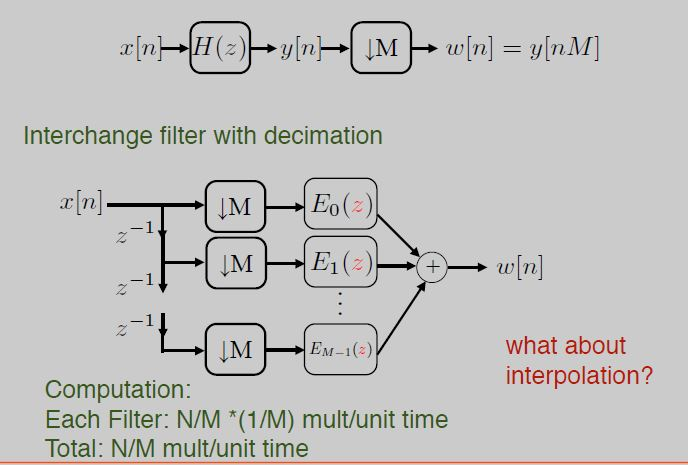
\includegraphics[scale = 0.5]{Figures/Multirate/polyphase_dowsampling}
\caption{Polyphase Structure}
\label{fig:Multirate:polyphase_dowsampling}
\end{figure}


\item Decompose our transfer function $H(z)$ into a sum of delayed transfer function which are compressed

\begin{equation}
H(z)\, = \, \displaystyle\sum_{k \, = \, 0}^{M \, - \, 1} E_k \left( \, z^M \, \right) \, z^{-k}
\end{equation}


\end{itemize}



\end{frame}


\subsection{Summary of Main Idea}


\begin{frame}[t]{Downsampling and Upsampling Ideas}

\begin{table}[!h]
\centering
	\begin{tabular}{|c|c|}
	\hline
		% header
		\multicolumn{2}{|c|}{Dowsampling}\\ \hline
		CTFT & DTFT \\ \hline
		
		Closer Images & Closer Images  \\ \hline
		
		Scaling Factor decrease & Scaling Factor decrease \\ \hline
		Bandwidth Same & Bandwidth Stretch \textcolor{blue}{but} still in $[\, - \, \pi , + \, \pi \,]$ \\ \hline		
	\end{tabular}
	\caption{Downsampling Operation Effects}
\end{table}

\end{frame}


%**************************************************
%**************************************************
%**************************************************



%------------ References ------------------------
\section{References}


\begin{frame}[allowframebreaks]
\frametitle{References}

\bibliographystyle{IEEEtran}
\frametitle{References}
\bibliography{Literature/Books_Signal_Processing,Literature/Communication_Systems,Literature/Papers_Signal_Processing}
\end{frame}


\end{document}
